\documentclass[12pt,          % font size: 11pt or 12pt
               phd,           % degree:    ms or phd
               onehalfspacing % spacing: onehalfspacing or doublespacing
               ]{ncsuthesis}

%%----------------------------------------------------------------------------%%
%%------------------------------ Import Packages -----------------------------%%
%%----------------------------------------------------------------------------%%

\usepackage{booktabs}  % professionally typeset tables
\usepackage{amsmath}
\usepackage{textcomp}  % better copyright sign, among other things
\usepackage{xcolor}
\usepackage{lipsum}    % filler text
\usepackage{longtable}
%\usepackage{subfig}    % composite figures
\usepackage{natbib}    % ability to use citet,citep
\usepackage{caption}        % for \captionof
\usepackage{subcaption}
%\usepackage{fancyhdr}  % creates headers
%\pagestyle{fancy}
\usepackage{subcaption}
%\usepackage{float}
%\usepackage[section]{placeins}
% Algorithms
\usepackage{algorithm}
\usepackage{algpseudocode}  % algorithmicx's "pseudocode" style
\usepackage{textcomp}  % better copyright sign, among other things
\usepackage{algorithmicx}  % for algorithm environments and indentation

% Optional niceties
\algrenewcommand\algorithmiccomment[1]{\hfill\(\triangleright\) #1}
\algrenewcommand\textproc{\textsf} % for \Call styling, if you use it
% Force floats to flush and start a new page after each algorithm
\newcommand{\AlgoPageBreak}{\FloatBarrier\clearpage}
\newcommand{\E}{\ensuremath{\mathcal{E}}}

 \usepackage{tabularx,booktabs,array,ragged2e,makecell}
% \newcolumntype{Y}{>{\raggedright\arraybackslash\ttfamily\footnotesize}X}
 \newcolumntype{Y}{>{\RaggedRight\arraybackslash}X}
 \newcolumntype{P}[1]{>{\RaggedRight\arraybackslash}p{#1}}


%Citations should be of the form ``author year''  not ``author, year''
\bibpunct{(}{)}{;}{a}{}{,} % changes apalike bst into AMS format
 
%%----------------------------------------------------------------------------%%
%%---------------------------- Formatting Options ----------------------------%%
%%----------------------------------------------------------------------------%%
%%

%% -------------------------------------------------------------------------- %%
%% Disposition format -- any titles, headings, section titles
%%  These formatting commands affect all headings, titles, headings,
%%  so sizing commands should not be used here.
%%  Formatting options to consider are
%%     +  \sffamily - sans serif fonts.  Dispositions are often typeset in
%%                    sans serif, so this is a good option. 
%%     +  \rmfamily - serif fonts
%%     +  \bfseries - bold face
%\dispositionformat{\sffamily\bfseries}   % bold and sans serif
\dispositionformat{\bfseries}            % bold and serif

%% -------------------------------------------------------------------------- %%
%% Formatting for centered headings - Abstract, Dedication, etc. headings
%%  This is where one might put a sizing command.
%%  \MakeUppercase can be used to typeset all headings in uppercase.
\headingformat{\large\MakeUppercase}   % All letters uppercase
%\headingformat{\large}                % Not all uppercase
%\headingformat{\Large\scshape}        % Small Caps, used with serif fonts.

%% Typographers recommend using a normal inter-word space after
%% sentences. TeX's default is to add an wider space, but \frenchspacing
%% gives a normal spacing. Comment out the following line if you prefer wider spaces between sentences.
\frenchspacing

%% -------------------------------------------------------------------------- %%
%%  Optional packages
%%    A number of compatible packages to improve the look and feel of
%%    your document are available in the file optional.tex 
%%    (For example, hyperlinks, fancy chapter headings, and fonts)
%% To use these options, uncomment the next line and see optional.tex
\include{optional}
%solve bug from fancyhdr in optional
%http://nw360.blogspot.com/2006/11/latex-headheight-is-too-small.html
\setlength{\headheight}{26.94345pt} % corrected error in Overleaf
\fancyhead[L]{\vspace{1mm}} % only puts chapter title in headers

%%----------------------------------------------------------------------------%%
%%---------------------------- Content Options -------------------------------%%
%%----------------------------------------------------------------------------%%
%% Size of committee: 3, 4, 5, or 6 -- this number includes the chair
\committeesize{5}

%% Members of committee
%%  Each of the following member commands takes an optional argument
%%   to specify their role on the committee.
%%  For co-chairs, use the commands:
%%      \cochairI{Doug Dodd}
%%      \cochairII{Chris Cox}
%%
\chair{Chair first and last name}
\memberI{Member 1 name}
\memberII{Member 2 name}
\memberIII{Member 3 name}   % unnecessary if committeesize=3
\memberIV{Member 4 name}    % unnecessary if committeesize=3, 4

%% Student writing thesis, \student{First Middle}{Last}
\student{First name and Middle names}{Last Name} % a full middle name

%% Degree program e.g. Marine, Earth, and Atmospheric Science
\program{program name}

%%!!!!!! To Change Year !!!!!!%%
% If year of graduation is not same as current year (common for December graduates
% thanks to the Grad Schools odd graduation rules) go into ncsuthesis.cls and change 
% \the\year in the line:
% \newcommand{\ncsu@year}{\the\year}
% to the year of graduation. E.g.:
% \newcommand{\ncsu@year}{2020}

%% Thesis Title
%%  Keep in mind, according to ETD guidelines:
%%    +  Capitalize first letter of important words.
%%    +  Use inverted pyramid shape if title spans more than one line.
%%
%%  Note: To break the title onto multiple lines, use \break instead of \\.
%\thesistitle{A North Carolina State University Sample \LaTeX{} Thesis \break 
%with a Title So Long it Needs a Line Break}
\thesistitle{Dissertation title}

%% Degree year. Necessary if your degree year doesn't equal the current year.
%\degreeyear{1995}

%% While your here make sure to change the PDF characteristics in optional.tex!!!

%%----------------------------------------------------------------------------%%
%%---------------------------- Personal Macros -------------------------------%%
%%----------------------------------------------------------------------------%%

%% A central location to add your favorite macros.

%% A few examples to get you started.
\newcommand{\uv}[1]{\ensuremath{\mathbf{\hat{#1}}}}
\newcommand{\bo}{\ensuremath{\mathbf{\Omega}}}
\newcommand{\eref}[1]{Eq.~\ref{#1}}
\newcommand{\fref}[1]{Fig.~\ref{#1}}
\newcommand{\tref}[1]{Table~\ref{#1}}

%%---------------------------------------------------------------------------%%
\begin{document}
%%---------------------------------------------------------------------------%%
\frontmatter

%% ------------------------------ Abstract ---------------------------------- %%
\begin{abstract}

Persistent faults in non-volatile memory, such as flash or ROM, pose a major threat to system reliability. Unlike transient upsets in volatile state, these errors alter the stored program image and reappear across every boot, often disabling recovery during system initialization. Existing compiler-based methods focus on transient data-path faults and provide little protection once instruction bytes in static memory are corrupted.

This thesis examines software-based strategies to improve the reliability of instruction memory through code repair and code replication, coordinated by pre-execution validation. Repair reconstructs corrupted regions algorithmically, while replication replaces damaged code with validated alternatives. Together, these methods strengthen execution continuity when parts of the program image are compromised. The work evaluates their effects on performance, reliability, storage cost, and code overhead, identifying the trade-offs that determine when each approach is most effective for embedded and safety-critical systems.

\end{abstract}


%% ---------------------------- Copyright page ------------------------------ %%
%% Comment the next line if you don't want the copyright page included.
\makecopyrightpage

%% -------------------------------- Title page ------------------------------ %%
\maketitlepage

%% -------------------------------- Dedication ------------------------------ %%
%\begin{dedication}
% \centering To my parents.
%\end{dedication}

%% -------------------------------- Biography ------------------------------- %%
%\begin{biography}
%The author was born in a small town \ldots
%\end{biography}

%% ----------------------------- Acknowledgements --------------------------- %%
\begin{acknowledgements}
Thanks to family, advisor, committee, office friends, etc. ...
\end{acknowledgements}


\thesistableofcontents

\thesislistoftables

\thesislistoffigures


%%---------------------------------------------------------------------------%%
\mainmatter

% Chapters can remove or add
\chapter{Introduction}
\label{chap:intro}

Computer systems do not operate in a single moment. They execute across time, and their ability to function correctly must hold from the first cycle to the last. A system begins execution in a defined initial state, but as operations accumulate and memory is accessed repeatedly, the likelihood of deviation from intended behavior increases. Every computation depends on fetching instructions and reading or writing data, and each access introduces the possibility of corruption. Reliability therefore is not simply about beginning correctly; it is about remaining correct until the task has completed. Programs that run longer, access more memory, or execute more instructions experience greater exposure to potential failure. A system must maintain coherent operation from its initial state at startup through all subsequent steps, and instability at any point before completion can prevent it from achieving the intended outcome.

The earliest moments of execution are particularly sensitive. At power-on, the system begins running initialization code that transitions it from reset into a usable operating context. During this phase, the processor first consumes instructions and data without yet having confidence in their correctness. Any disturbance in these initial accesses, whether to instruction bytes or configuration values, can disrupt progress, corrupt early state, trigger repeated resets, or halt execution before meaningful work begins. The system therefore starts in an \emph{unqualified memory state}, and its primary challenge is to advance far enough to establish a \emph{qualified memory state} in which continued execution can proceed with a high likelihood of correctness. Until that transition occurs, each memory access carries elevated risk, and failure can prevent the system from ever reaching stable operation.

The central challenge, and the focus of this work, is to increase the probability that a system reaches a qualified memory state even in the presence of memory upsets, mutations, or corruptions. The methods developed here aim to raise the likelihood that early execution continues long enough to establish stability and transition into a trusted operating mode. In effect, the problem is one of \emph{bootstrapping reliability}: enabling a system to move from an unqualified memory state into one where execution can proceed with confidence, despite the possibility that some stored instructions or data differ from their intended form.

\section{Background}
\label{sec:background}

Ensuring long-term system dependability requires mechanisms that limit the impact of memory corruption as it accumulates over time. These mechanisms fall into two broad categories: hardware techniques built into the platform and software techniques applied above the architecture. Hardware mechanisms operate continuously and transparently, reducing error rates within the bounds anticipated by the system design. Software can complement these defenses by providing additional resilience when faults exceed those bounds or occur in regions not fully protected by hardware. Together, these layers form the basis for sustained reliable operation.

\subsection{Hardware-Based Approaches}

Hardware reliability features are intended to preserve stable behavior in the presence of physical memory faults. These capabilities are implemented in memory structures, processor pipelines, and interconnects, and operate automatically at runtime. When fault rates remain within the system's assumptions, hardware can significantly limit the likelihood that corrupted values propagate into execution.

Error-correcting codes (ECC) detect and correct a bounded number of bit flips by storing additional redundancy alongside memory words. Memory scrubbers may proactively scan memory to repair correctable faults before they accumulate. As long as errors stay within the correction capacity, memory reads continue to reflect their expected values.

Lock-step execution provides another protection strategy by running identical instructions on multiple processor cores and comparing outputs cycle-by-cycle. Divergence between the cores signals a fault and prompts error handling or safe shutdown. Such mechanisms are common in high-assurance settings where correctness is prioritized over resource cost.

These techniques significantly reduce error exposure but operate within finite design margins. ECC corrects only a limited number of bit errors; beyond that boundary, corruption may escape detection or propagate silently. Lock-step execution detects computational divergence but does not prevent slow accumulation of corruption in instruction or data memory. Over long deployments, persistent or gradually accumulating memory faults may eventually exceed hardware protections. At that point, additional layers must assist in preserving dependable execution.

\subsection{Software-Based Approaches}

Software techniques provide a second line of defense when memory integrity cannot be fully guaranteed by hardware alone. Unlike physical redundancy mechanisms, software methods require no special fabrication or memory features and can be deployed on existing platforms at compile time or runtime. Their purpose is to manage execution behavior when faults occur, increasing the likelihood that the system continues to operate correctly or fails in a controlled manner.

Two broad strategies are used: detection and recovery.

\begin{itemize}
  \item \textbf{Detection} identifies when program behavior deviates from expectations. It may take the form of consistency checks on control flow, validation of stored values, or cross-checking between redundant computations. Detection does not directly correct state; it provides awareness that an upset has occurred so the system can react deliberately instead of unknowingly propagating corruption.

  \item \textbf{Recovery} aims to bias execution toward correct behavior even in the presence of faults. It uses structural or algorithmic redundancy so that when disturbances occur, execution remains aligned with the intended program logic. Recovery may reconstruct values from encoded representations, select among multiple candidate results, or apply transformations that preserve expected semantics. Rather than responding only after failure, recovery increases the probability that execution continues along a valid trajectory despite disturbances.
\end{itemize}

While hardware techniques provide essential protection against memory disturbances, they cannot always ensure correct execution over long operational lifetimes, especially as stored state gradually mutates or exceeds correction limits. Software mechanisms offer a complementary path: they operate above the physical substrate and can be deployed without modifying the underlying hardware. Because they can be adapted, tuned, or introduced at any point in a system's lifetime, software-based approaches can reinforce execution even when hardware protection is minimal or aging.

Software reliability techniques broadly pursue two goals: recognizing when execution deviates from expectations and increasing the likelihood that execution remains correct despite disturbances. Together, detection and recovery can significantly improve reliability by identifying inconsistencies and maintaining forward progress in spite of faults. These methods do not depend on hardware configuration or fabrication constraints and can therefore extend reliability beyond the limits of physical memory protection. In this work, we focus on software-based mechanisms that increase the probability a system reaches and maintains a stable operating state, even as memory content mutates over time.

\subsection{Related Work}

Software reliability techniques typically harden either the data path, the instruction path, or both. These approaches work by controlling how memory is used and verified so that stored and computed values remain aligned with intended program state, even when memory disturbances occur.

\textbf{Data-path hardening} ensures that values stored in and loaded from memory remain correct. A widely used approach is \emph{shadow memory}, where each memory region is replicated in one or more shadow regions. On every load, the system retrieves values from all replicas and resolves them through a convergence filter that biases execution toward the intended value. On every store, all copies are updated in parallel, maintaining structural alignment across regions. When a disturbance affects one location, the replicated layout prevents error amplification and maintains consistent state. Other methods use encoded computation, such as AN-codes, to detect mutations by embedding arithmetic structure into stored values.

\textbf{Instruction-path hardening} protects the control and execution flow. Control flow checking assigns lightweight signatures to basic blocks and verifies them at entry to detect illegal jumps or unexpected transitions. Execution redundancy replicates dependence chains and compares computed results at runtime. Deviations indicate incorrect behavior and lead to recovery or controlled halt, maintaining expected program direction and correctness during execution.

Some systems combine both instruction and data protection. \emph{SWIFT-R} is one example, integrating replicated execution chains with shadow memory to reinforce correctness across the entire execution pipeline. This coupling increases resilience by ensuring that both the data state and the execution trajectory remain consistent, even when memory upsets occur.

Most state-of-the-art reliability mechanisms rely on a \emph{post-execution detection strategy}, where faults must first occur before they can be recognized and recovered. This model works reasonably well for data, since corrupted values can often be detected or corrected after they are read. For instructions, however, this assumption becomes a critical limitation. If corrupted instructions must execute in order to trigger detection or recovery, the system may already have lost control flow or corrupted its internal state beyond repair. Furthermore, many instruction-hardening schemes increase fault exposure indirectly: by duplicating or triplicating dependence chains, they inflate the instruction stream and expand the portion of memory that must remain fault-free for recovery logic to function. As a result, mechanisms intended to improve resilience can inadvertently reduce the probability of successful recovery.

This work instead focuses on \emph{pre-execution validation}, seeking to identify and neutralize corrupted instructions before they are executed. The goal is to raise the probability that early execution proceeds through trustworthy code regions, allowing the system to reach a stable, qualified state even when underlying memory contains latent upsets or mutations.

A practical example of pre-execution validation already exists in the form of the \emph{A/B image strategy} used in many embedded ARM systems. This method maintains two complete firmware images—designated A and B—stored in non-volatile memory. During boot, the system inspects each image and selects one to execute based on integrity checks or update status. Although primarily designed for safe firmware updates, this mechanism inherently supports fault tolerance. If both images are functionally identical, one can serve as a verified fallback when corruption is detected in the other. The same concept can be extended beyond two images—maintaining multiple replicas increases the probability that at least one remains uncorrupted and executable. By validating and selecting the execution target before any instruction is fetched, such multi-image schemes satisfy the principle of pre-execution validation: code is qualified prior to use, and execution proceeds only from trusted regions of memory.

The progression of these techniques reflects a shift toward proactive reliability, qualifying code and data before they are executed rather than responding after faults occur. Replication-based methods, such as multi-image validation, demonstrate one way to achieve this early assurance. The following section introduces another perspective, comparing replication with repair as complementary strategies for establishing qualified memory before execution begins.

\section{Replication vs. Repair}
\label{sec:replication-vs-repair}

Replication and repair represent two complementary strategies for maintaining reliable operation in the presence of memory upsets.

Replication preserves multiple functionally identical variants of code or data and selects among them at runtime. The granularity can range from entire program images to individual bytes. Below the image level, access must pass through a layer of indirection: a lookup table holds references to valid replicas, and all reads or calls are routed through this table. For data, each memory operation is redirected through the table so that loads and stores target a qualified copy. For instructions, calls and branches entering or leaving a protected region are resolved through the same indirection mechanism, ensuring execution proceeds only through verified variants.

Repair, in contrast, operates in place. Rather than selecting among alternatives, it reconstructs or corrects corrupted memory directly. Proactive repair can resolve faults down to the bit level without altering the instruction stream. It depends on two main design factors: redundancy and complexity. Redundancy provides the extra information needed to restore the original state, while complexity determines the time and code cost of performing that restoration. Together, these form a three-way trade-off among redundancy, computational effort, and achievable reliability.

At finer granularity, repair typically outperforms replication. Replication requires that every bit in the protected region remain correct in at least one copy; any corruption in all replicas of the same position leads to failure. Repair, by contrast, uses available redundancy to reconstruct missing or altered information, making more efficient use of stored data. Because of this, repair should be applied as soon as the system environment allows modification or rewriting of memory. The next section examines how system constraints influence the choice and timing of each strategy.

\section{System Architecture and Memory Constraints}
\label{sec:system-architecture}

System architecture plays a central role in determining which reliability strategies can be applied and how effective they are. The nature of the memory hierarchy, including its volatility, accessibility, and organization, defines the practical limits of replication and repair.

Dynamic memory elements, including caches, registers, and RAM, are volatile by design. Their contents are cleared after each power cycle, which naturally removes any accumulated corruption. In such memory, recovery mechanisms focus primarily on detection. Once corruption is identified, a reset or reinitialization can restore correct state without permanent loss. Persistent protection is therefore less critical, since faults do not survive across reboots.

Static memory, in contrast, retains its contents across power cycles and exists in both writable and read-only forms. Repair requires write access, which makes it infeasible for regions that are permanently locked or physically read-only. Writable static memory, such as flash, introduces additional constraints. Flash memory cannot be read and written simultaneously within the same region and requires a program--erase (P/E) cycle to modify data. As a result, code responsible for repair cannot safely reside in the same section that is being rewritten. For instruction repair, coherence hazards may also arise if cached instruction data is modified without appropriate synchronization. These conditions are typically managed by hardware mechanisms that support self-modifying code but impose strict operational ordering.

Memory organization also shapes the feasibility of both replication and repair. Figure~\ref{fig:harvard-von-neumann} compares the Harvard and Von~Neumann architectures. In a Von~Neumann architecture, instructions and data share the same address space, allowing software to generate or modify executable code dynamically. This flexibility supports both instruction and data repair at runtime. In a Harvard architecture, instructions and data reside in physically separate memory spaces. Stores cannot target instruction memory, restricting repair to data regions only. While this separation improves security by preventing unintended code modification, it also prevents in-place instruction repair.

\begin{figure}[t]
  \centering
  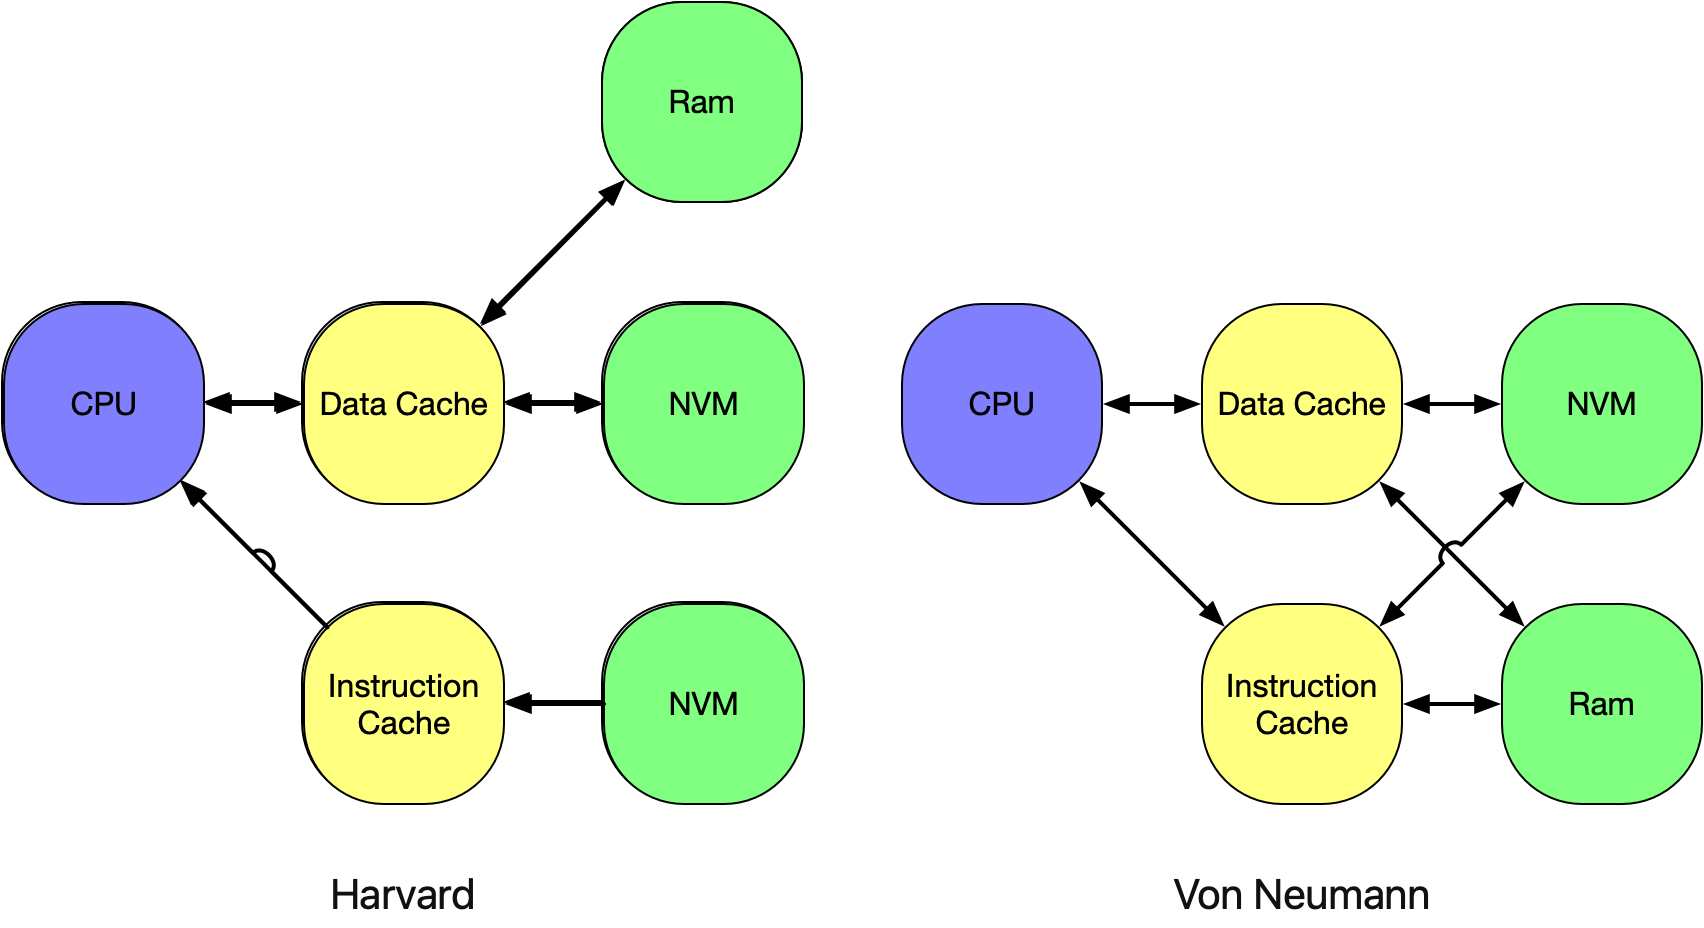
\includegraphics[width=0.9\linewidth]{Chapter-1/figs/HarvardxVon.png}
  \caption{Comparison between Harvard and Von~Neumann architectures. Harvard systems maintain distinct physical memory paths for instructions and data, improving security and predictability but preventing runtime modification of instruction memory. Von~Neumann systems share a unified address space, allowing both instructions and data to coexist and be modified dynamically, enabling flexible software-based repair but introducing potential reliability risks from shared corruption sources.}
  \label{fig:harvard-von-neumann}
\end{figure}

Hybrid architectures combine elements of both. They maintain separate instruction and data spaces for security-critical components while allowing writable or unified memory for dynamic regions. In hybrid designs, read-only sections are a deliberate design decision. In most embedded systems, execution proceeds in two phases: a read-only bootloader stored in ROM and a writable bootloader stored in flash. Some systems include internal flash memory on-chip that can control which medium or image is used for the next boot phase. These mixed designs require selective application of reliability mechanisms, using replication for immutable instruction areas and repair for writable data and code regions where modification is permissible.


\section{Motivation and Focus of This Work}
\label{sec:motivation}

The distinction between dynamic and static memory defines where reliability mechanisms can operate effectively. Dynamic memory is inherently recoverable: its contents are volatile, and corruption can be cleared simply by resetting the system or refetching data from a trusted source. Post-execution validation methods therefore work well in this domain, and extensive research has established effective strategies for detecting and correcting transient faults.

Static memory, by contrast, retains its contents across resets, making it a long-term source of unrecoverable faults. Errors in these regions persist and reappear every time the program executes. Figures~\ref{fig:section-breakdown-m2} and~\ref{fig:section-breakdown-embedded} show the normalized composition of representative binaries collected from an Apple-based general-purpose system and an Arduino-class embedded processor. In both cases, the majority of bytes reside in the \texttt{.text} section, which contains executable instructions. The \texttt{.rodata} and \texttt{.data} sections, while smaller, are mutable or copyable into RAM during initialization and can therefore be repaired using conventional techniques. Instruction memory, however, dominates the static footprint and cannot be trivially rewritten or refreshed once execution begins.

This gap defines the central focus of this work. While data reliability is well understood and broadly supported by existing software and hardware mechanisms, instruction reliability remains a critical weakness. The remainder of this thesis evaluates two complementary strategies for improving the survivability of instruction memory: \textbf{replication}, which provides multiple alternate copies for redirection, and \textbf{repair}, which reconstructs corrupted code in place. Together, these approaches aim to increase the probability that execution can continue successfully even when faults occur in static program storage.

\begin{figure}[t]
  \centering
  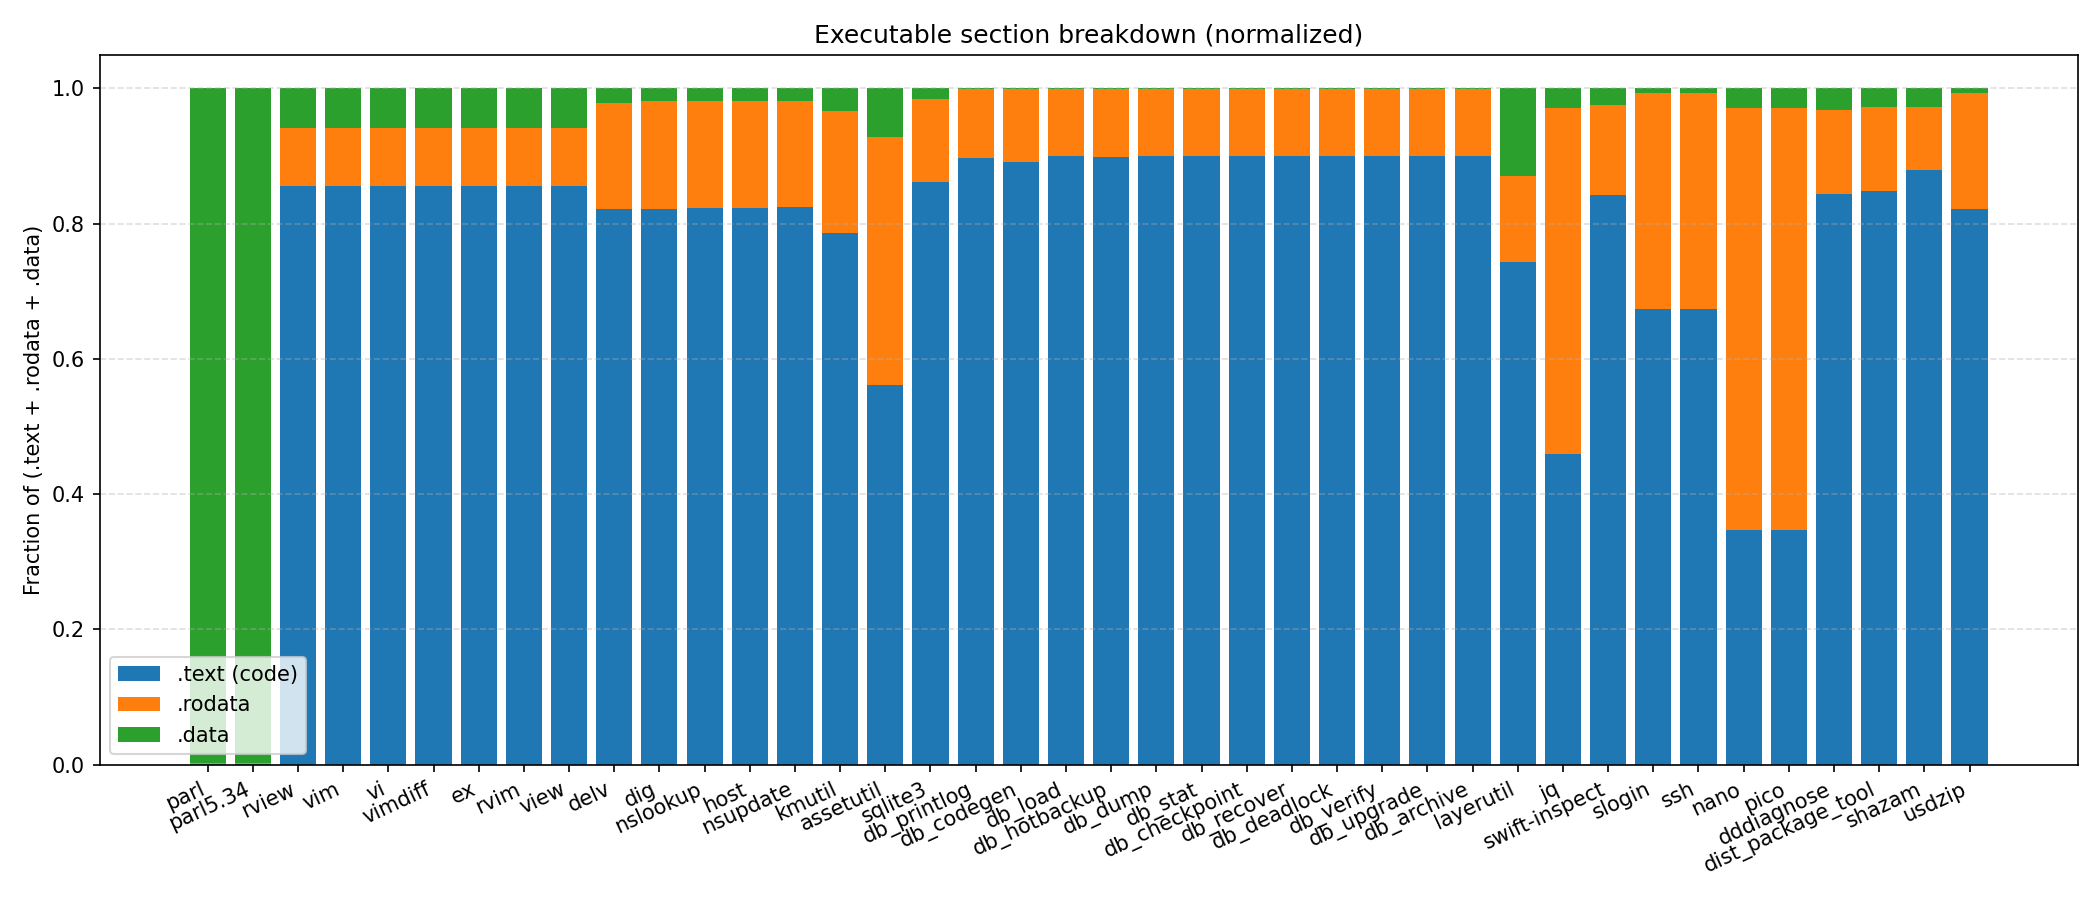
\includegraphics[width=0.9\linewidth]{Chapter-1/figs/apple-bin.png}
  \caption{Executable section breakdown of representative user-space binaries compiled for an Apple-based general-purpose system. The \texttt{.text} section dominates the static footprint, with \texttt{.rodata} and \texttt{.data} contributing smaller fractions.}
  \label{fig:section-breakdown-m2}
\end{figure}

\begin{figure}[t]
  \centering
  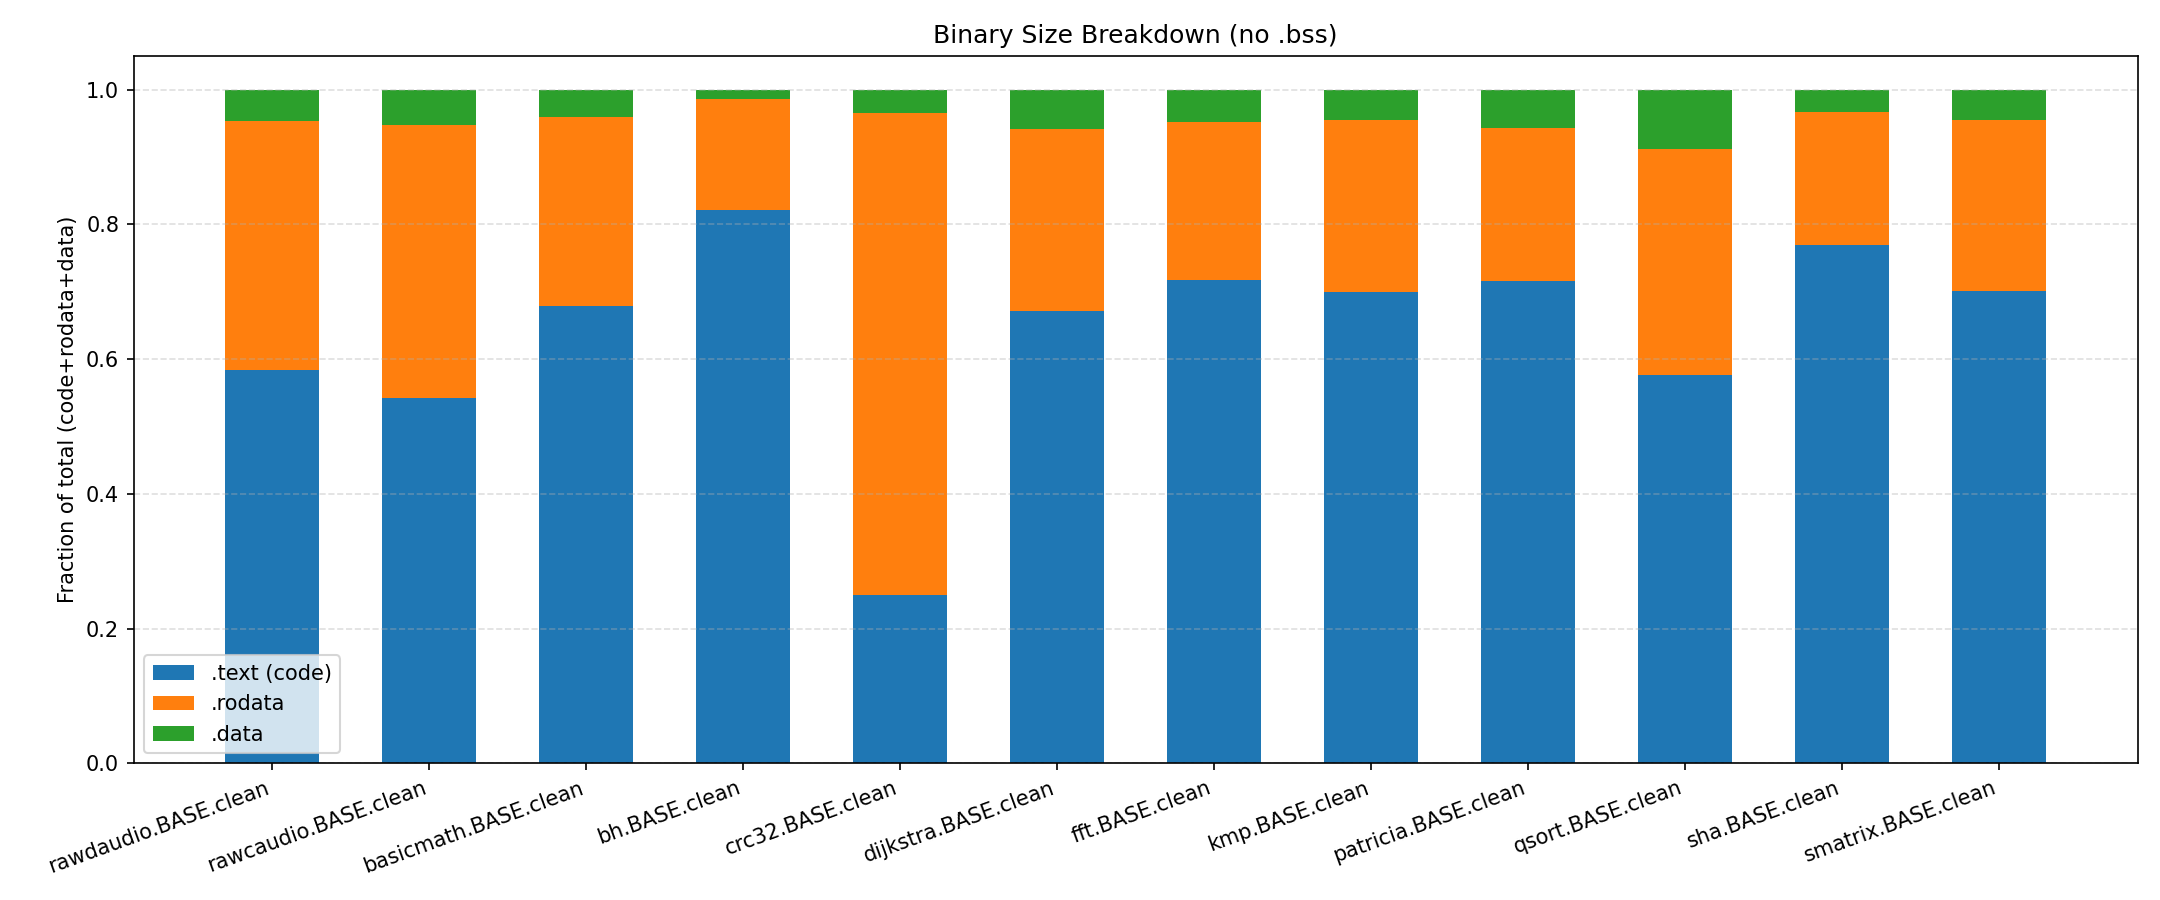
\includegraphics[width=0.9\linewidth]{Chapter-1/figs/embedded-bin.png}
  \caption{Executable section breakdown of representative embedded benchmarks compiled for an Arduino-class processor. Similar to general-purpose systems, code regions dominate the static memory footprint.}
  \label{fig:section-breakdown-embedded}
\end{figure}
\chapter{Fault Characterization and Observation}
\label{chap:fault-model}

Persistent faults in static memory are the central concern of this work. 
Transient faults that arise in dynamic elements—such as registers, caches, or SRAM—are short-lived and typically disappear after a reset or rewrite. 
In these cases, detection and restart are sufficient to restore correct operation. 
In contrast, \textbf{static memory}—such as flash, ROM, EEPROM, or other non-volatile storage—retains errors across resets and power cycles. 
A corrupted instruction or data word in these regions permanently alters program behavior, making persistence rather than transience the defining property of the reliability challenge.




Figure~\ref{fig:system-diagram} illustrates a representative embedded microcontroller architecture.
The CPU serves as the execution core, surrounded by memory and peripheral subsystems. 
Program memory contains the executable instructions that define control flow, while RAM stores transient computation state. 
EEPROM often holds configuration or calibration data that is written infrequently but read frequently.
From a reliability perspective, these three types of memory exhibit distinct fault behavior. 
RAM faults are ephemeral and can usually be cleared through reset, whereas EEPROM and flash-based program memory retain corruption indefinitely.
This persistence makes them the dominant source of long-term reliability degradation in embedded devices.

\begin{figure}[t]
  \centering
  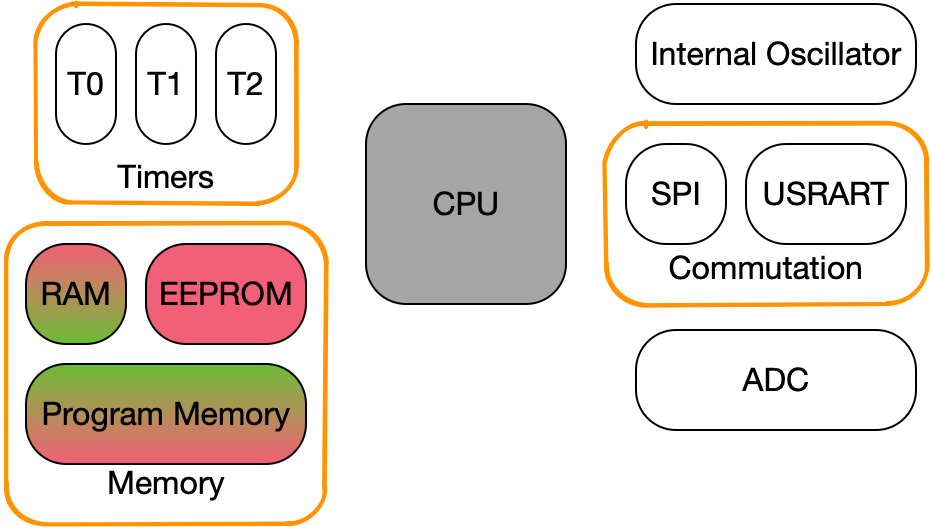
\includegraphics[width=0.85\linewidth]{Chapter-2/figs/system-diagram.png}
  \caption{
  Simplified microcontroller architecture highlighting major subsystems where faults may arise.
  The CPU interfaces with three key memory components: volatile \textbf{RAM}, semi-persistent \textbf{EEPROM}, 
  and non-volatile \textbf{program memory} (typically flash or ROM). 
  Peripheral units such as timers, communication interfaces (SPI, USART), and the ADC rely on correct instruction and data delivery from these memories.
  Transient faults primarily affect dynamic regions such as RAM or registers, while faults in EEPROM or flash persist across reboots, directly threatening long-term system reliability.
  }
  \label{fig:system-diagram}
\end{figure}

\section{Overview of Fault Types}
\label{sec:fault-types}

Faults in computing systems can be grouped by duration and repeatability:

\begin{itemize}
  \item \textbf{Transient faults} are short-lived disturbances caused by radiation, voltage fluctuations, or environmental interference. They affect the current state but vanish after a reset or overwrite.
  \item \textbf{Intermittent faults} recur under specific operational or environmental conditions—such as temperature or voltage stress—but are not permanently fixed in hardware.
  \item \textbf{Persistent faults} alter the stored representation of the program or data. They remain present until the affected memory is explicitly rewritten or replaced.
\end{itemize}

While transient and intermittent faults degrade runtime stability, persistent faults have far more severe implications for embedded and long-lived systems. 
They can render a device permanently unreliable, even when transient protection mechanisms such as ECC, replay, or watchdog recovery are active.

\section{Fault Localization in the Memory Hierarchy}
\label{sec:fault-localization}

The likelihood and impact of faults vary with their position in the memory hierarchy. 
Dynamic memories such as SRAM hold ephemeral runtime data, while non-volatile storage retains the permanent program image. 
Static regions—including \texttt{.text}, \texttt{.rodata}, and the pre-initialized portion of \texttt{.data}—are loaded or executed directly from persistent memory. 
Any corruption in these sections introduces \textbf{deterministic faults}: each fetch or load reproduces the same error on every execution.

By contrast, transient upsets in volatile state—such as a flipped register bit—are naturally overwritten during program progress and rarely persist. 
This distinction makes static instruction and data segments the dominant risk surface for persistent reliability failures.

\section{Statistical Fault Model}
\label{sec:statistical-model}

We model reliability beginning at the cell level. 
Let $p_f$ denote the probability that a single memory cell is faulty, with faults assumed to occur independently across cells. 
For a memory block containing $M$ cells, the probability that the entire block is fault-free is:

\begin{equation}
p_{\mathrm{free}} = (1 - p_f)^M
\end{equation}

The complementary probability that the block contains at least one fault is:

\begin{equation}
p_{\mathrm{fail}} = 1 - (1 - p_f)^M
\end{equation}

This relationship shows the exponential sensitivity of reliability to block size. 
Even when $p_f$ is extremely small, increasing $M$ rapidly reduces the chance that the entire block remains fault-free. 
For small $p_f$, the approximation $p_{\mathrm{fail}} \approx M \cdot p_f$ reveals the linear dependence of failure likelihood on block size in the low-fault regime.

\begin{figure}[t]
  \centering
  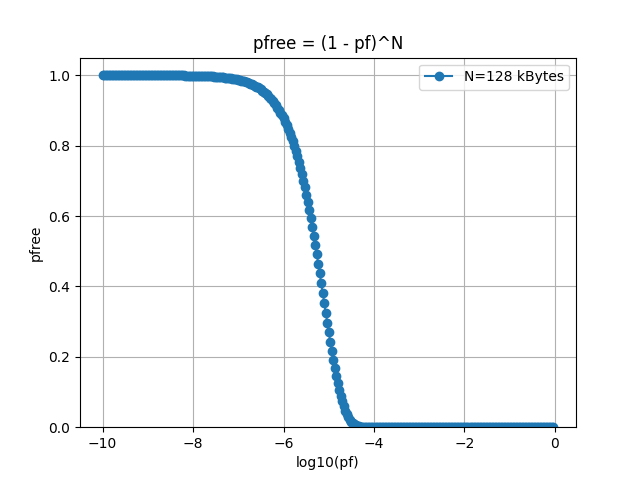
\includegraphics[width=0.90\linewidth]{Chapter-2/figs/pfree.png}
  \caption{System survival probability $p_{\mathrm{free}}$ versus per-cell fault probability $p_f$ for a 128~kB memory region. 
  The logarithmic scale highlights the sharp reliability collapse as $p_f$ increases beyond $10^{-8}$.}
  \label{fig:pfree}
\end{figure}

When plotted for a 128~kB region, reliability remains nearly perfect while $p_f$ is below about $10^{-10}$, but collapses rapidly once $p_f$ rises beyond $10^{-8}$. 
By $10^{-4}$, the chance of a fault-free region is effectively zero. 
This steep ``S-curve'' illustrates how even modest increases in bit-error probability can lead to catastrophic unreliability in large memories.

\section{Raw vs. Unrecoverable Error Rates}
\label{sec:raw-vs-uer}

The per-cell probability $p_f$ represents the \textit{raw error rate} of the underlying technology. 
In practice, systems employ multiple layers of mitigation—such as Error-Correcting Codes (ECC), redundancy, or block replacement—that mask or repair many faults before they affect execution. 
The rate that remains after correction is the \textit{unrecoverable error rate (UER)}.

The difference between the raw error rate and the UER reflects the strength of the protection mechanism. 
A robust ECC scheme can tolerate most single-bit and some multi-bit faults, lowering the effective UER by several orders of magnitude. 
Weak or absent protection leaves the UER nearly equal to $p_f$. 
Thus, while the raw error rate gives a device-level measure of reliability, the UER determines the operational reliability of the system as experienced by software.

These models provide the analytical foundation for evaluating how faults in static memory propagate through software systems. 
The next chapter builds on this foundation by examining how an unprotected system behaves under injected faults, establishing a baseline against which repair and replication mechanisms can be measured.
\chapter{Baseline System Reliability}
\label{chap:baseline-reliability}

This chapter establishes the behavior of an unprotected system under instruction-memory faults. 
It serves as a lower bound for achievable reliability before the introduction of any repair, replication, 
or validation mechanisms. The results define how rapidly reliability collapses when executable code 
in persistent storage is corrupted.

\section{Overview}
\label{sec:baseline-overview}

An unprotected system assumes that the stored program image is correct. 
Any corruption in the instruction stream---such as a flipped opcode, altered branch target, 
or modified immediate value---directly changes control flow or semantics during execution. 
Because these faults reside in non-volatile storage, they persist across resets and power cycles. 
Each boot reintroduces the same corrupted bytes, making failure behavior deterministic rather than transient.

This chapter quantifies how such systems degrade when instruction memory becomes unreliable. 
The analysis provides a baseline reference against which all later fault-tolerant mechanisms are evaluated.

\section{Fault Model Recap}
\label{sec:baseline-fault-model}

The reliability model follows the probabilistic framework developed in Chapter~\ref{chap:fault-model}. 
Each memory byte has an independent probability of corruption, and the number of corrupted bytes 
within a region follows a Poisson distribution with mean $\frac{M}{R}$, 
where $M$ is the region size and $R$ the average spacing between faults.

For this baseline study, faults are injected exclusively into the \texttt{.text} section, 
which contains executable instructions. 
The \texttt{.data} and \texttt{.rodata} sections remain intact. 
This isolates the sensitivity of the instruction path from effects related to dynamic data or runtime variability. 
Each injected fault is treated as a permanent modification to non-volatile storage---representing 
a persistent instruction-level upset.

\section{Limit Study: Experimental Setup}
\label{sec:limit-study-setup}

The baseline limit study measures how system reliability changes as the density of instruction faults increases.  
The objective is to quantify the intrinsic fragility of executable code in isolation from other error sources.

\subsection*{Evaluation Platform}
All experiments were performed on an \textbf{x86-64 system} equipped with an 
\textbf{Intel(R) Core(TM) i7-8086K CPU @ 4.00 GHz}, executing in 
\textbf{64-bit little-endian mode}. 
Programs were compiled for the \textbf{x86-64 instruction set architecture}, 
and faults were applied to program images stored and executed from \textbf{main memory (DRAM)}. 
This configuration provides a consistent ISA model and deterministic execution environment for 
baseline fault-injection analysis.

\subsection*{Procedure}

\begin{enumerate}
  \item \textbf{Fault Injection:} 
  Each benchmark binary is processed by the injection function $I(R)$, which introduces 
  persistent bit flips within the \texttt{.text} section according to the Poisson--Uniform model. 
  Each injected fault permanently modifies an instruction byte, emulating a static corruption 
  in flash or ROM.

  \item \textbf{Execution:} 
  Corrupted binaries are executed directly on the host system with no redundancy, replay, 
  or error-handling mechanisms. 
  The program runs until normal completion or failure, and exceptions such as illegal instructions 
  or segmentation faults are logged.

  \item \textbf{Validation:} 
  Each run’s output is compared to the reference output from the fault-free binary. 
  Matching outputs are recorded as successful executions; mismatches, crashes, or hangs 
  are classified as failures.

  \item \textbf{Repetition:} 
  For each corruption rate $R$, the experiment is repeated across multiple independent trials 
  to capture statistical variation. 
  The mean success rate represents the empirical reliability of the unprotected instruction path.
\end{enumerate}

\subsection*{Scope of Evaluation}
Fault injection targets only the \texttt{.text} section. 
The \texttt{.data} and \texttt{.rodata} sections remain unmodified, ensuring that all effects measured 
arise solely from faults in executable instructions. 
This isolates the baseline sensitivity of instruction memory in the absence of protection mechanisms.

\section{Results and Observations}
\label{sec:limit-study-results}

At low fault densities, execution proceeds normally; corrupted instructions are rare, 
and the probability of encountering an altered opcode is negligible. 
As the expected number of corrupted bytes per program approaches one, reliability collapses sharply.  
Even a single corrupted instruction can cause a crash, an infinite loop, or silent output divergence.

The transition from reliable to unreliable execution follows a distinct three-region pattern:

\begin{itemize}
  \item \textbf{Stable region:} Faults are sparse and seldom strike active instructions; 
  execution remains correct.
  \item \textbf{Transition region:} The first critical instructions fail, causing control-flow errors 
  or computation divergence.
  \item \textbf{Collapse region:} Nearly all runs fail, as multiple faults disable essential code paths 
  or control logic.
\end{itemize}

Although this behavior is consistent across benchmarks, the exact collapse threshold varies with 
program structure. Control-intensive workloads, such as branching or function-heavy benchmarks, 
fail earlier than sequential compute kernels. Nevertheless, all show the same rapid loss of reliability 
once the average number of corrupted instructions approaches one per program image.

\begin{figure}[t]
  \centering
  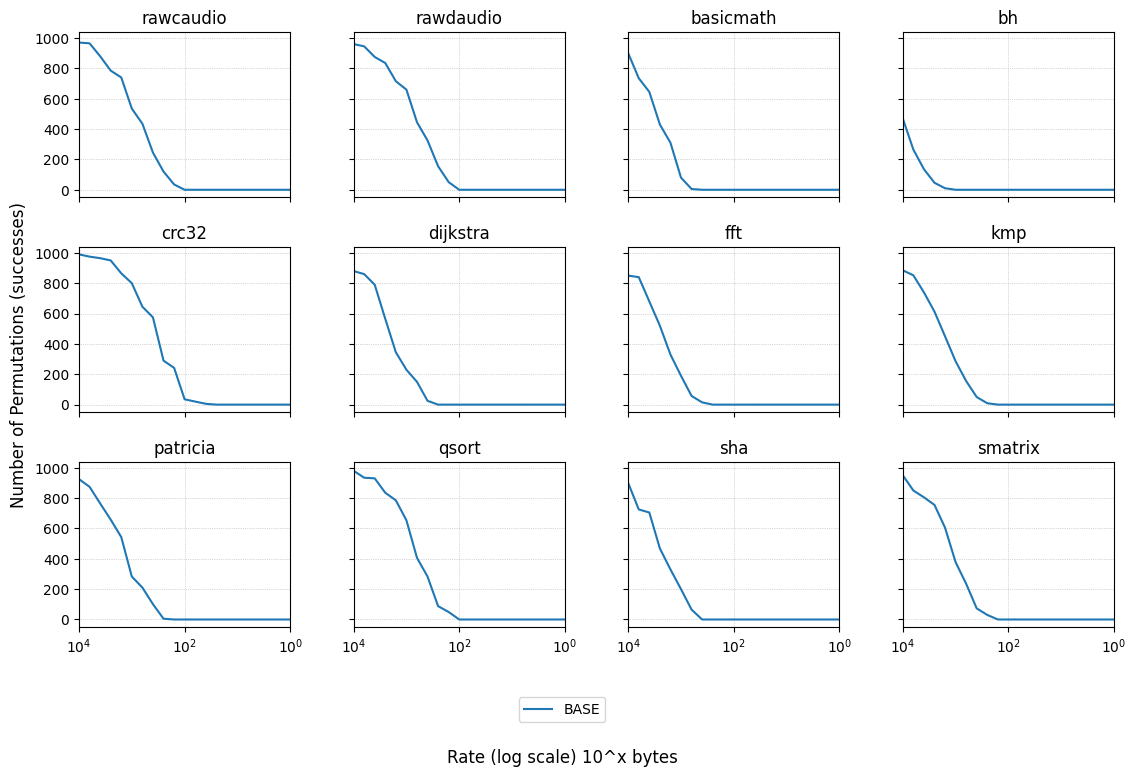
\includegraphics[width=0.90\linewidth]{Chapter-3/figs/baseline-reliability.png}
  \caption{Baseline limit study results showing reliability collapse as instruction faults increase. 
  Experiments executed on an Intel i7-8086K CPU (x86-64). 
  The x-axis shows the fault rate $\log_{10}(1/R)$; the y-axis shows the number of successful trials. 
  Reliability declines sharply once the expected number of corrupted instructions per program 
  approaches one.}
  \label{fig:baseline-reliability}
\end{figure}

\section{Interpretation}
\label{sec:limit-study-interpretation}

These results demonstrate that instruction memory is intrinsically fragile under persistent corruption.  
Even minimal, random instruction-level faults can permanently compromise system behavior, 
converting recoverable upsets into deterministic failures.  
Because the corrupted bytes persist across reboots, recovery through reset or replay is impossible; 
the system re-executes the same broken instruction sequence each time.

The baseline analysis therefore represents the natural limit of system reliability when no protection mechanisms are present.  
It defines a lower bound against which more advanced approaches can be compared.  
To surpass this boundary, a system must not only detect corruption but also regenerate usable code from damaged storage.  
Achieving this requires mechanisms capable of reconstructing functional instruction sequences directly within static memory---without reboot or external recovery.

\medskip
\noindent
The next chapter introduces one such approach: \textbf{recovery by repair}.  
Rather than leaving persistent faults unaddressed, repair techniques use redundancy and structured encoding 
to regenerate program content from corrupted data.  
This shift---from passive failure to active reconstruction---marks the first step toward self-sustaining reliability 
in persistent instruction memory.
% ==========================
\chapter{Recovery by Repair}
\label{chap:repair}
% ==========================

The unprotected limit study showed that instruction memory fails deterministically once faults persist in static storage. 
Resets and detection mechanisms provide no recovery because corrupted instructions are re-executed identically after every reboot. 
This behavior defines the lower bound of software reliability—where faults in code itself permanently prevent progress.  

To move beyond detection, the system must regenerate correct behavior from within the same faulty memory space. 
\textbf{Repair} achieves this by algorithmically reconstructing code or data from redundant or overlapping information, 
producing a more reliable version of the original content. 
Unlike reset-based recovery, repair operates in place, fusing imperfect data to restore an executable state.  

This chapter introduces repair as the first active recovery mechanism for static memory faults. 
It evaluates two representative models—\textbf{Majority-of-3} and \textbf{Reed–Solomon (255,223)}—that combine information from multiple unreliable regions to reconstruct usable code. 
Both approaches operate entirely within memory, without reboot or external reprogramming, and aim to restore a coherent instruction stream by reinforcing correct content through redundancy.  

% ---------------------------------------------------
\section{Overview}
\label{sec:repair-overview}
% ---------------------------------------------------

The following sections develop a quantitative model of repair, derive analytical expressions for survivability, 
and validate these models through a limit study that measures how repair strength and redundancy influence system reliability. 
These results establish repair as a baseline mechanism for sustaining execution when persistent instruction corruption 
would otherwise render the system non-recoverable.

\section{Repair Survivability}
\label{sec:repair-survivability}

Repair mechanisms improve system survivability by introducing structured redundancy into static memory.  
They increase the likelihood that usable code or data can be reconstructed directly from within the same faulty region.  
Each protected area contains two main components: a \textit{source block} that holds the original content and one or more \textit{redundant blocks} that encode overlapping or supplementary information derived from it.  
When corruption occurs, these blocks are combined algorithmically to form a reconstructed version that has a higher probability of being correct than any individual block alone.

Two representative forms of repair are considered: \textbf{Majority-of-3} replication and the \textbf{Reed--Solomon (255,223)} code.  
Both rely on redundancy but differ in structure, efficiency, and computational cost.  

\subsection{Majority-of-3}

Majority-of-3 is a replication-based approach in which three identical copies of each bit are stored.  
During repair, the most common value among the three is selected, allowing a correct bit to be recovered as long as two of the three replicas remain uncorrupted.  
This scheme is simple and effective against isolated bit errors but requires significant storage overhead—two-thirds of all stored bits are redundant.

Let $p_f$ denote the probability that a single bit is faulty.  
For any given bit position, let $X \sim \mathrm{Binomial}(3, 1 - p_f)$ represent the number of fault-free replicas.  
The fused bit is fault-free if $X \ge 2$, giving the per-bit survivability:

\begin{equation}
P_{\text{bit,maj3}} = \sum_{k=2}^{3} \binom{3}{k} (1 - p_f)^k p_f^{3-k} = 1 - 3p_f^2 + 2p_f^3.
\end{equation}

If $S$ bytes of memory are protected by Majority-of-3, the total number of fused bits is $\tfrac{8S}{3}$, yielding whole-memory survivability:

\begin{equation}
p_{\text{free,maj3}}(S, p_f) = (1 - 3p_f^2 + 2p_f^3)^{\tfrac{8S}{3}}.
\end{equation}

This model captures how redundancy statistically suppresses bit-level faults but with a steep storage penalty.

\subsection{Reed--Solomon (RS(255,223))}

Reed--Solomon repair uses an algebraic method that distributes data and parity across groups of bytes.  
When a subset of these bytes becomes corrupted, missing or invalid data can be regenerated mathematically using the remaining bytes, provided the number of errors does not exceed the correction capacity of the code.  
The RS(255,223) configuration stores 223 data bytes and 32 parity bytes per codeword, achieving approximately 87\% efficiency and tolerating up to 16 corrupted bytes per block.

Let $p_f$ again denote the per-bit fault probability, and define the per-byte fault probability as:

\begin{equation}
q = 1 - (1 - p_f)^8.
\end{equation}

The probability that an RS(255,223) codeword is decodable—that is, that it contains at most 16 faulty bytes—is:

\begin{equation}
p_{\text{block,RS}}(q) = \sum_{j=0}^{16} \binom{255}{j} q^j (1 - q)^{255-j}.
\end{equation}

For a protected memory of size $S$ bytes, the number of full codewords is:

\begin{equation}
N_{\text{RS}} = \left\lceil \frac{S}{255} \right\rceil,
\end{equation}

and the total memory survivability is:

\begin{equation}
p_{\text{free,RS}}(S, p_f) = \left( p_{\text{block,RS}}(q) \right)^{N_{\text{RS}}}.
\end{equation}

This form shows how Reed--Solomon maintains high survivability until its correction threshold is exceeded, after which reliability collapses sharply.

\begin{figure}[t]
  \centering
  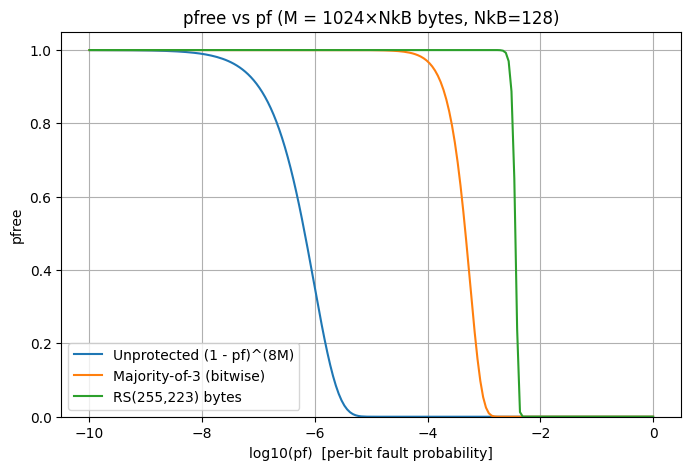
\includegraphics[width=\linewidth]{Chapter-4/figs/pfree-reed_maj.png}
  \caption{Modeled survivability of Majority-of-3 and Reed--Solomon (255,223) repair for a 128~kB memory region.  
  Each curve shows the probability of complete fault-free recovery as a function of per-bit fault probability $p_f$.  
  Both methods combine information from multiple unreliable \textit{source blocks} and their associated \textit{redundant blocks} to reconstruct usable data.  
  Majority-of-3 degrades gradually with fault density, while Reed--Solomon maintains near-perfect reliability until its decoding capacity is exceeded.}
  \label{fig:pfree-vs-pf-128kb}
\end{figure}

\subsection{Comparison and Interpretation}

Figure~\ref{fig:pfree-vs-pf-128kb} compares survivability for the two repair schemes over a 128~kB memory region.  
Both extend reliability several orders of magnitude beyond the unprotected baseline, but their behavior diverges under increasing corruption.  
Majority-of-3 exhibits a smooth, probabilistic decline as more replicas fail, while Reed--Solomon maintains a sharp threshold—perfect recovery below its correction limit and sudden collapse beyond it.  
This contrast illustrates the design trade-off between simplicity and efficiency: replication offers continuous but costly improvement, whereas coding provides near-ideal protection up to a fixed limit.  

These analytical results form the upper bound of repair performance.  
The following section empirically validates these models through controlled fault injection, measuring how closely practical repair aligns with the theoretical predictions.

\section{Limit Study}
\label{sec:ch3-limit-study}

The repair limit study quantifies how practical repair mechanisms behave when faults are directly injected into memory.  
While the analytical model predicts ideal survivability under the assumption of independent faults and perfect correction, 
this experiment measures how these theoretical benefits hold under real program conditions.  
It represents the transition from mathematical reliability to empirical system behavior.

In this study, both \textbf{Majority-of-3} and \textbf{Reed--Solomon (RS 255,223)} repair schemes are evaluated using 
the same probabilistic fault model introduced earlier.  
The per-bit fault probability is fixed at its maximum ($p_f = 1$), representing a fully fault-saturated environment.  
Rather than varying $p_f$ directly, the experiment varies the \textbf{injection rate} $R$, which defines the average 
spacing between corrupted bytes.  
Smaller $R$ values correspond to denser corruption, while larger $R$ values represent sparser, more isolated faults.  
This approach allows each repair mechanism’s reliability limit to be observed under progressively worsening fault density.

Each repair mechanism operates on a set of encoded binary images derived from the benchmark programs.  
The experimental workflow consists of four phases:

\begin{enumerate}
  \item \textbf{Encoding} – Each benchmark is transformed into a protected format using either Majority-of-3 replication 
  or Reed--Solomon coding.  
  The encoder generates redundant structures representing \textit{source} and \textit{redundant} blocks.

  \item \textbf{Fault Injection} – Corruption is applied to these encoded images following the Poisson--Uniform model.  
  Only the encoded memory is corrupted; decoder executables remain fault-free to isolate the effects of repair.

  \item \textbf{Decoding (Repair)} – Each corrupted image is decoded using its corresponding algorithm.  
  Majority-of-3 performs bitwise voting across replicas, while Reed--Solomon reconstructs codewords algebraically.

  \item \textbf{Validation} – The repaired outputs are executed and compared against known-good results.  
  Successful runs indicate complete and correct reconstruction, while mismatches or crashes indicate repair failure.
\end{enumerate}

\begin{figure}[t]
  \centering
  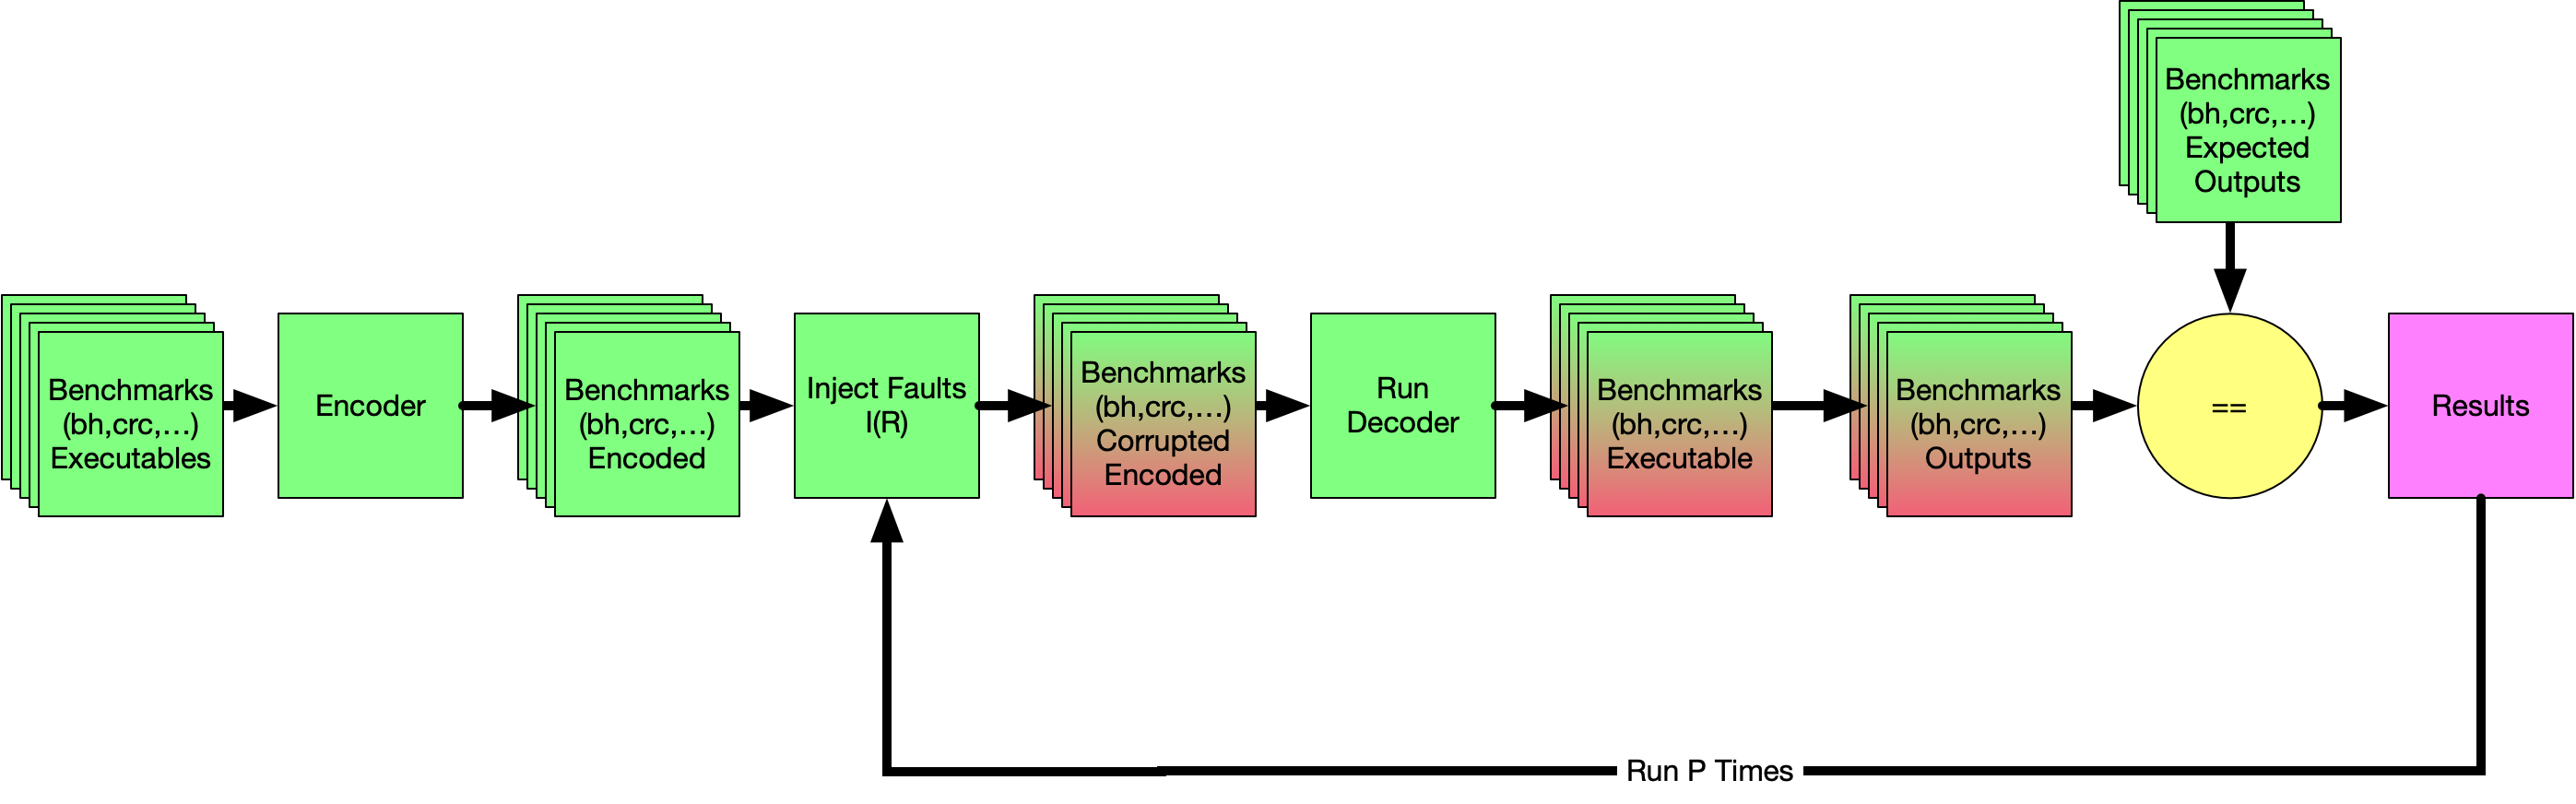
\includegraphics[width=\linewidth]{Chapter-4/figs/repair-flow.png}
  \caption{Repair limit-study workflow. Benchmarks are first \emph{encoded} (producing source and redundant blocks), then faults are \emph{injected} into the encoded images according to the Poisson--Uniform model. The corrupted images are \emph{decoded (repaired)}, yielding executable binaries that are run to produce outputs. Outputs are compared to known-good references; equality counts as success. The entire process is repeated \(P\) times per injection rate \(R\) to obtain empirical survivability.}
  \label{fig:repair-flow}
\end{figure}

The process is repeated multiple times for each injection rate $R$ to capture statistical variation.  
For each configuration, the fraction of successful reconstructions represents the measured system survivability.

\begin{figure}[t]
  \centering
  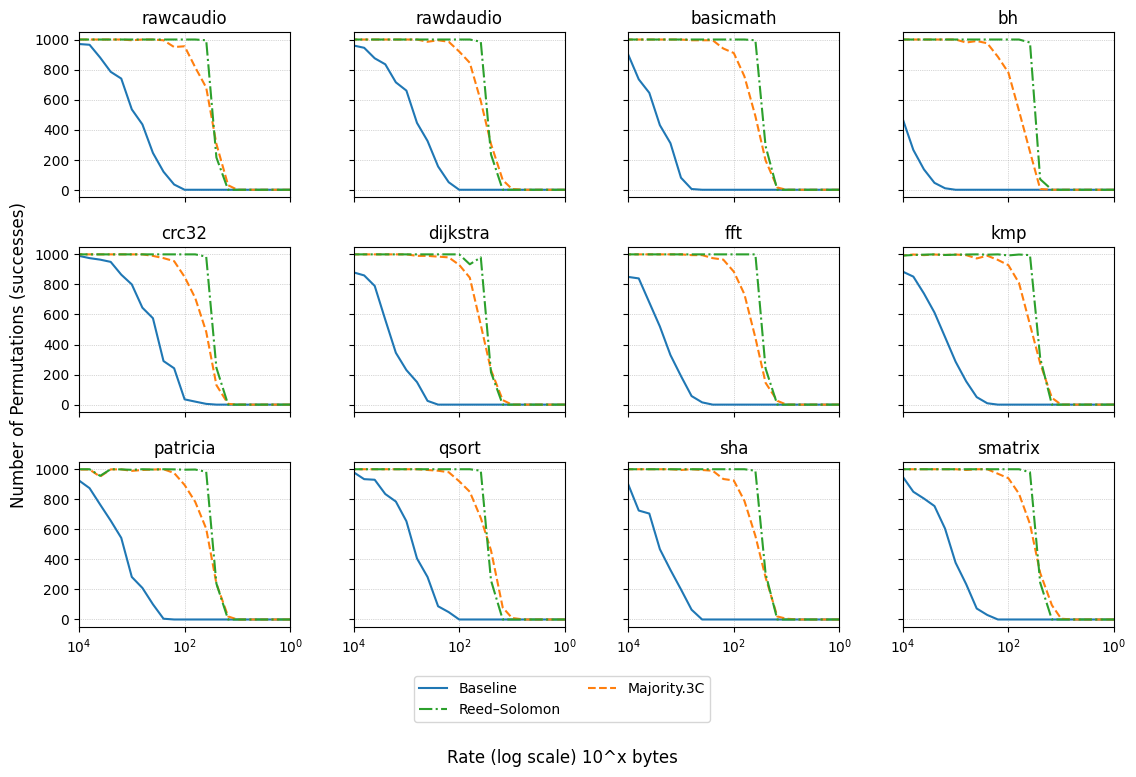
\includegraphics[width=\linewidth]{Chapter-4/figs/repair-reliability.png}
  \caption{Repair limit study results across benchmarks: number of successful permutations (out of $P$) versus injection rate $R$ (log scale).  
  Curves shown for Majority-of-3 and Reed--Solomon repair.  
  Both methods significantly extend functional survivability relative to the unprotected baseline.}
  \label{fig:repair-limit-results}
\end{figure}

\subsection{Results and Interpretation}
\label{subsec:ch3-limit-results}

The results show two distinct reliability profiles.  
\textbf{Majority-of-3} repair degrades gradually as the injection rate increases.  
Even under dense corruption, a fraction of systems continue to operate correctly because the probability of majority agreement remains nonzero.  
This produces a smooth, continuous decline in survivability, consistent with the probabilistic fusion of multiple noisy replicas.

\textbf{Reed--Solomon}, by contrast, exhibits a sharp threshold.  
For injection rates below its correction capacity, it achieves near-perfect reconstruction; once the number of corrupted bytes 
exceeds the 16-byte correction limit per codeword, reliability collapses almost instantaneously.  
This behavior matches the analytical model’s prediction: Reed--Solomon acts as a high-efficiency, high-risk boundary—
exceptionally effective within its limit but brittle beyond it.

Compared to the unprotected baseline, both methods extend survivability by several orders of magnitude.  
Reed--Solomon maintains integrity deeper into fault density, while Majority-of-3 offers graceful degradation rather than abrupt failure.  
Together, these results demonstrate the fundamental trade-off between replication and algebraic repair:  
replication consumes more memory to achieve continuity, while coding achieves higher efficiency at the cost of a strict correction boundary.

The repair limit study confirms that real-world repair follows the theoretical trends established in the analytical model.  
It also defines the practical boundaries of survivability—how redundancy interacts with fault density, how correction capacity scales, 
and where the probability of successful reconstruction drops below viability.  
These insights provide the foundation for applying repair in embedded systems, 
where memory access restrictions and runtime constraints further determine the feasibility of in-place recovery.

% ---------------------------------------------------
\section*{Repair Boundaries and the Need for Redirection}
% ---------------------------------------------------

While repair demonstrates that faulty code can sometimes be reconstructed from within the same memory space, 
its success depends on both the availability and integrity of writable regions. 
Even when a device supports in-system writes, the underlying memory cells may no longer accept updates once degraded—%
faults can permanently prevent the intended write or erase operation from succeeding. 
When this occurs, repair becomes ineffective because the correction cannot be physically applied.  
In these situations, reliability must come from structural redundancy rather than regeneration.  
The next chapter introduces \textbf{redirection by code replication}, in which multiple validated copies of code are pre-placed in memory, 
and execution dynamically shifts among them when corruption is detected.  
This approach extends survivability beyond the limits of repair by rerouting control flow through verified instruction paths 
instead of attempting to rewrite damaged storage.
% ==========================
\chapter{Code Replication}
\label{chap:code-replication}
% ==========================

\textbf{Code replication} extends the concept of repair by redirecting execution
around faulty memory regions. Instead of reconstructing corrupted instructions
in place, replication ensures that alternate copies of the same code exist
elsewhere in memory. If one region fails, control can be transferred to another
region containing a fault-free replica.

Replication thus provides a software-level form of spatial redundancy,
preserving functional continuity even when static memory becomes partially
unreliable. The following sections develop a probabilistic model of replicated
code survivability and introduce a hierarchy of replication granularities.

% ---------------------------------------------------
\section{Replication Survivability Model}
\label{sec:replication-model}
% ---------------------------------------------------

Let $p_f$ denote the probability that a single bit in memory is faulty.
Each replicated code region contains $R$ bytes, or $8R$ bits.
The probability that an individual region remains completely fault-free is

\begin{equation}
p_{\text{region}} = (1 - p_f)^{8R}.
\end{equation}

Suppose a section of code is replicated $N$ times across different regions.
The section is usable if at least one replica remains intact.
Let $X$ be the number of fault-free replicas:

\begin{equation}
X \sim \mathrm{Binomial}(N,\, p_{\text{region}}).
\end{equation}

Then the section’s fault-free probability is

\begin{equation}
p_{\text{section}} = P(X \ge 1)
  = 1 - (1 - p_{\text{region}})^{N}
  = 1 - \Big[1 - (1 - p_f)^{8R}\Big]^{N}.
\end{equation}

For total protected code space $S$, divided into $M = S/(RN)$
independent sections, the overall system survivability is

\begin{equation}
\boxed{
p_{\text{free,total}}(S, R, N, p_f)
  = \Big[1 - \big(1 - (1 - p_f)^{8R}\big)^{N}\Big]^{\tfrac{S}{RN}}.
}
\end{equation}

For small $p_f$, $(1 - p_f)^{8R} \!\approx e^{-8Rp_f}$,
showing how survivability increases exponentially with replica count $N$.

\begin{figure}[t]
  \centering
  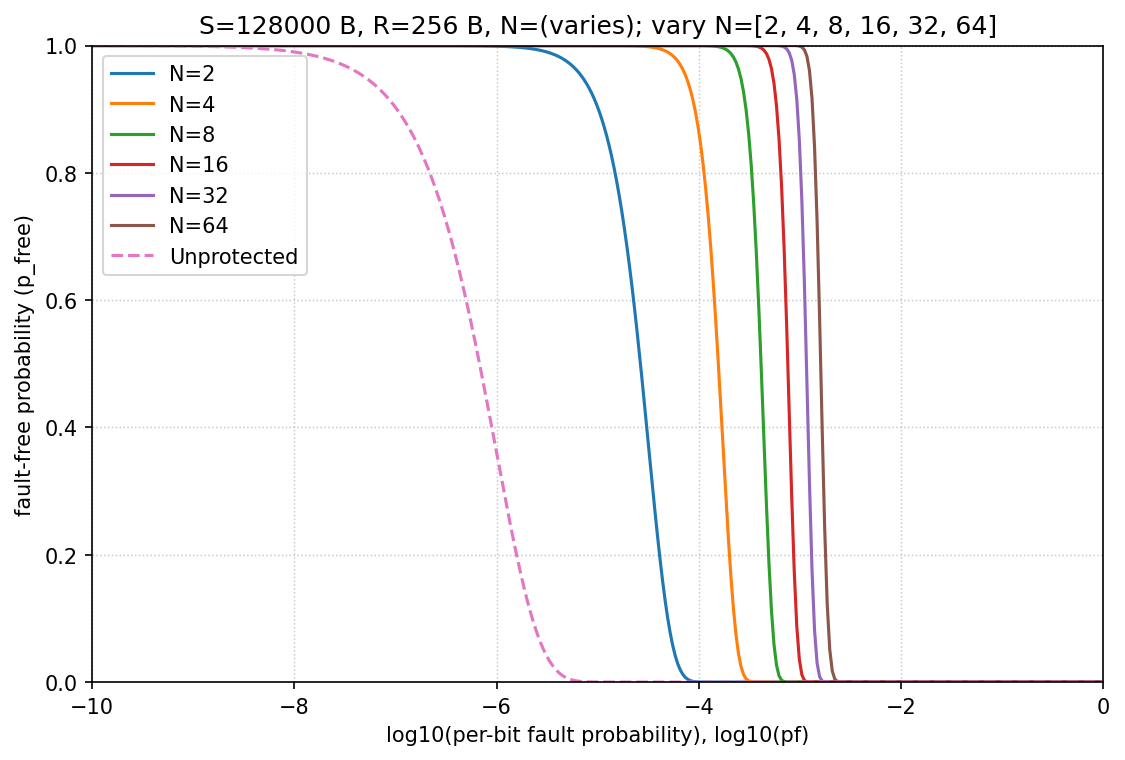
\includegraphics[width=\linewidth]{Chapter-5/figs/pfree_R256_N2_16.png}
  \caption{$p_{\text{free}}$ vs.\ $p_f$ for total memory
           $S=128\,\mathrm{kB}$, fixed region size $R=256$\,B, and
           varying replication count
           $N\in\{2,4,8,16,32,64\}$. Increasing $N$ extends the
           survivability plateau before reliability collapse.}
  \label{fig:varN}
\end{figure}

\begin{figure}[t]
  \centering
  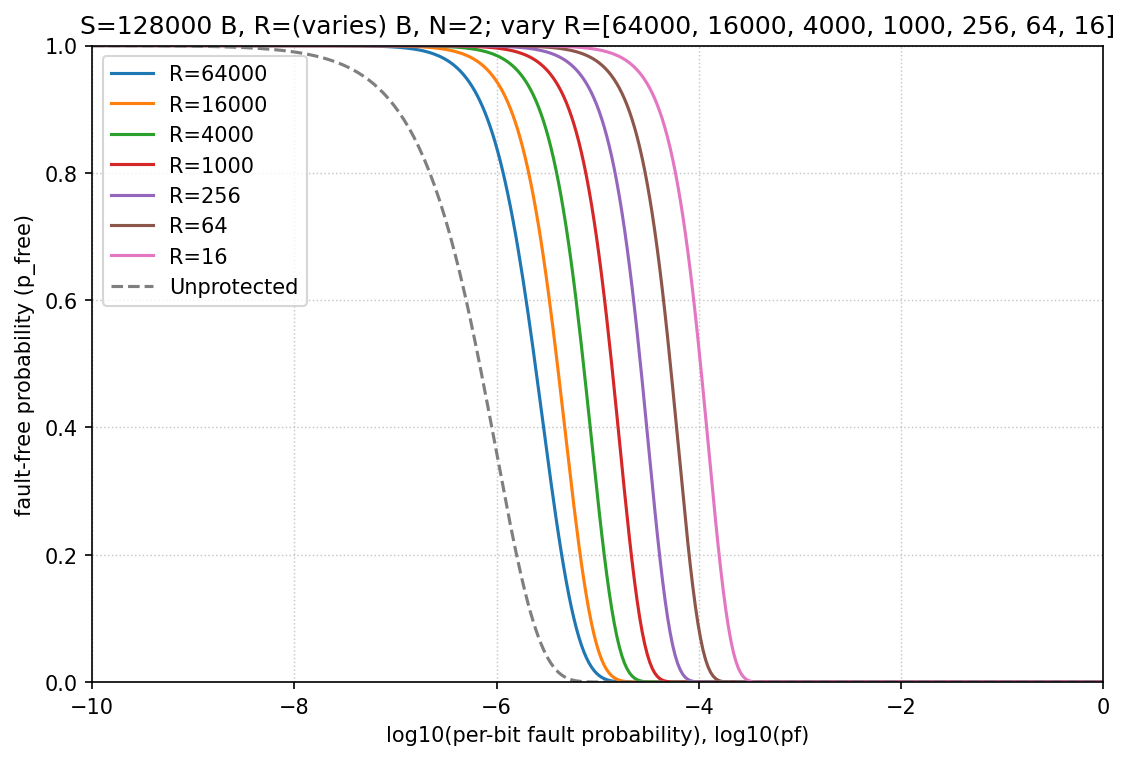
\includegraphics[width=\linewidth]{Chapter-5/figs/pfree_R64k_16_N2.png}
  \caption{$p_{\text{free}}$ vs.\ $p_f$ for total memory
           $S=128\,\mathrm{kB}$, fixed replication count $N=16$,
           and varying region size
           $R\in\{1,2,4,8,16,64\}\,\mathrm{kB}$. Smaller $R$ values
           yield higher survivability due to greater independence.}
  \label{fig:varR}
\end{figure}

These results show that increasing $N$ (replica count) or reducing $R$
(region size) improves the likelihood that at least one intact replica remains.
Smaller regions, however, increase metadata and redirection overhead, defining
a trade-off between granularity and efficiency.

% ---------------------------------------------------
\section{Replication Granularity}
\label{sec:replication-granularity}
% ---------------------------------------------------

Code replication can be organized at multiple \textit{granularities}—each
representing a distinct balance between redundancy cost, validation complexity,
and fault-isolation precision.  Table~\ref{tab:replication-granularity}
summarizes the four principal levels evaluated in this work.

\begin{table}[t]
  \centering
  \small
  \renewcommand{\arraystretch}{1.15}
  \caption{Granularity levels of code replication.}
  \label{tab:replication-granularity}
  \begin{tabularx}{\linewidth}{@{}l P{3.2cm} Y Y@{}}
    \toprule
    \textbf{Granularity} & \textbf{Protected Unit} &
    \textbf{Redirection Mechanism} & \textbf{Typical Use} \\
    \midrule
    Region-Level (RLCR) &
    Entire program image or code partition &
    Startup validation and region selection before execution begins &
    Bootloaders, firmware fallback partitions, redundant ROM images \\

    Function-Level (FLCR) &
    Individual functions &
    Call-site indirection through a validated function table (\texttt{ITab}) &
    Modular executables, dynamic linking, selective runtime recovery \\

    Basic-Block-Level (BBLCR) &
    Control-flow basic blocks &
    Runtime branch redirection through validated block targets (\texttt{BTab}) &
    Fine-grained fault isolation, localized instruction-path recovery \\

    Instruction-Level (ILCR) &
    Individual instructions or micro-sequences &
    On-the-fly reconstruction of instruction bytes followed by immediate
    invocation through generated trampolines or stubs &
    Extreme fault localization; recovery when higher structures are corrupted \\
    \bottomrule
  \end{tabularx}
\end{table}

The hierarchy proceeds from coarse static redundancy (RLCR) to highly dynamic,
self-modifying recovery (ILCR). Each level builds on the previous one by tightening
the granularity of validation and redirection.

% ---------------- RLCR ----------------
\subsection*{Region-Level Code Replication (RLCR)}
At the coarsest level, an entire program image or code region is replicated.
A startup validation routine verifies each region’s integrity and selects the
first valid image for execution. Once a valid region is chosen, execution
proceeds directly within it—no further control-flow indirection is required.
RLCR trades memory capacity for simplicity and is widely used in dual-image
bootloaders and redundant firmware updates.

% ---------------- FLCR ----------------
\subsection*{Function-Level Code Replication (FLCR)}
FLCR divides the program into independently replicated functions.
Indirection occurs only at function-call boundaries, where each call
resolves to a validated function replica before transferring control.
Within a function, execution proceeds directly with no additional
redirection.

% ---------------- BBLCR ----------------
\subsection*{Basic-Block-Level Code Replication (BBLCR)}
BBLCR refines FLCR by introducing indirection at basic-block boundaries.
Each branch or jump target is resolved at runtime to a verified replica,
while instructions within a basic block execute directly.
This fine-grained indirection enables execution to bypass damaged code
regions within a function and continue safely through valid paths.

% ---------------- ILCR ----------------
% ---------------- ILCR ----------------
\subsection*{Instruction-Level Code Replication (ILCR)}
At the finest granularity, ILCR reconstructs instructions dynamically rather
than redirecting among existing blocks. Short instruction sequences are
regenerated from redundant encodings or reference data, placed into writable
memory, validated, and immediately invoked via a temporary trampoline.
Because execution enters synthesized code directly, ILCR behaves like a
disciplined form of self-modifying code.

This capability requires several architectural conditions:

\begin{itemize}
  \item \textbf{Writable or relocatable code space:}
        Reconstructed instructions must reside in a writable and executable
        memory region, or the system must relocate code dynamically into such
        a space at runtime.

  \item \textbf{No PC-relative addressing:}
        Reconstructed sequences must avoid PC-relative addressing or be fully
        position-independent, since relocation invalidates absolute offsets.
        All references must be expressed through registers or absolute pointers.

  \item \textbf{Controlled reconstruction:}
        Each reconstructed fragment is verified for integrity before execution
        and discarded or replaced after completion, preventing uncontrolled
        self-modification.
\end{itemize}

At this granularity, ILCR resembles a form of \textbf{code repair} rather than
traditional replication. Because its mechanisms focus on dynamic regeneration
and repair rather than redirection among preexisting copies, ILCR lies beyond
the scope of the replication-focused analysis in this study.

% ---------------------------------------------------
\section{Summary}
\label{sec:replication-summary}
% ---------------------------------------------------

This chapter established the analytical foundation of code replication and its
hierarchical structure. The probabilistic model quantified how redundancy
parameters ($R$, $N$) determine survivability, while the granularity taxonomy
(RLCR, FLCR, BBLCR) illustrates how runtime control-flow management evolves—
from region-level selection through function-call redirection to basic-block-level
edge resolution.

Across all three levels, the total amount of redundant code storage remains
constant; what differs is the point in the control flow where redirection
occurs. RLCR performs selection at the region boundary, FLCR redirects at
function-call sites, and BBLCR introduces indirection at basic-block edges.
This progression refines how faults are isolated and bypassed without increasing
replication overhead.

The following chapters examine each level in detail:
\begin{itemize}
  \item Chapter~\ref{chap:region-level} — \textbf{Region-Level Replication (RLCR)}
        enabling recovery through region-level selection at runtime.
  \item Chapter~\ref{chap:flcr} — \textbf{Function-Level Replication (FLCR)}
        introducing call-site redirection to isolate faults within specific
        functions.
  \item Chapter~\ref{chap:bblcr} — \textbf{Basic-Block-Level Replication (BBLCR)}
        extending redirection to intra-function control flow for fine-grained
        fault recovery.
\end{itemize}

Together, these mechanisms form a continuum of software-based fault-tolerance
strategies, in which finer granularities provide greater control-flow resilience
without additional redundancy cost, but at the expense of increased runtime
and management complexity.
% ===================================================
\chapter{Region-Level Code Replication (RLCR)}
\label{chap:region-level}
% ===================================================

\section{Overview}
Region-Level Code Replication (RLCR) represents the broadest form of software redundancy.
At this level, the entire program image---or a major executable region---is duplicated in full.
Each region contains a complete, self-consistent copy of all code and static data required for execution.
During initialization, a validation routine examines each region to verify its integrity (e.g., via checksum or hash).
Once a valid region is identified, control is transferred to its entry point, and all subsequent execution proceeds entirely within that region.
Because all addresses within a region are internally consistent, no runtime indirection is required after the selection step.

\section{Mechanism}
RLCR operation consists of three stages: replication, validation, and selection.

\paragraph{Replication.}
Redundant regions are produced during the build process, where identical program images are generated and placed at distinct memory addresses.
Each image can be stored in separate non-volatile segments.

\paragraph{Validation.}
At startup, an integrity check is performed for each region.
This routine determines which copy remains intact and therefore safe for execution.

\paragraph{Selection.}
After validation, the system activates the valid region by updating the program counter or vector-table base to the region's start address.
From that point forward, all execution uses fixed absolute addresses within the selected copy.

\begin{figure}[t]
  \centering
  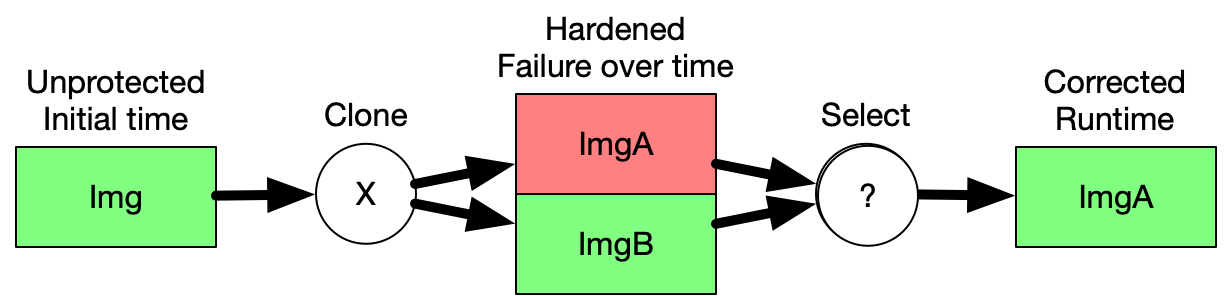
\includegraphics[width=\linewidth]{Chapter-6/figs/dual-image-mechanism.png}
  \caption{Dual-image RLCR mechanism.
           Two identical program regions (ImgA and ImgB) occupy distinct memory ranges.
           On startup, each region is validated; if one fails integrity checks, execution proceeds from the other.
           After a valid region is selected, control remains within that region without further indirection.}
  \label{fig:rlcr-dual}
\end{figure}


\section{Execution Sequence}
Figure~\ref{fig:rlcr-seq} illustrates the loader/selector flow for RLCR.
A minimal loader image performs initialization, invokes a selector when multiple images are present, and then transfers control to the selected program region.
After selection, execution continues entirely within the chosen region.

\begin{figure}[t]
  \centering
  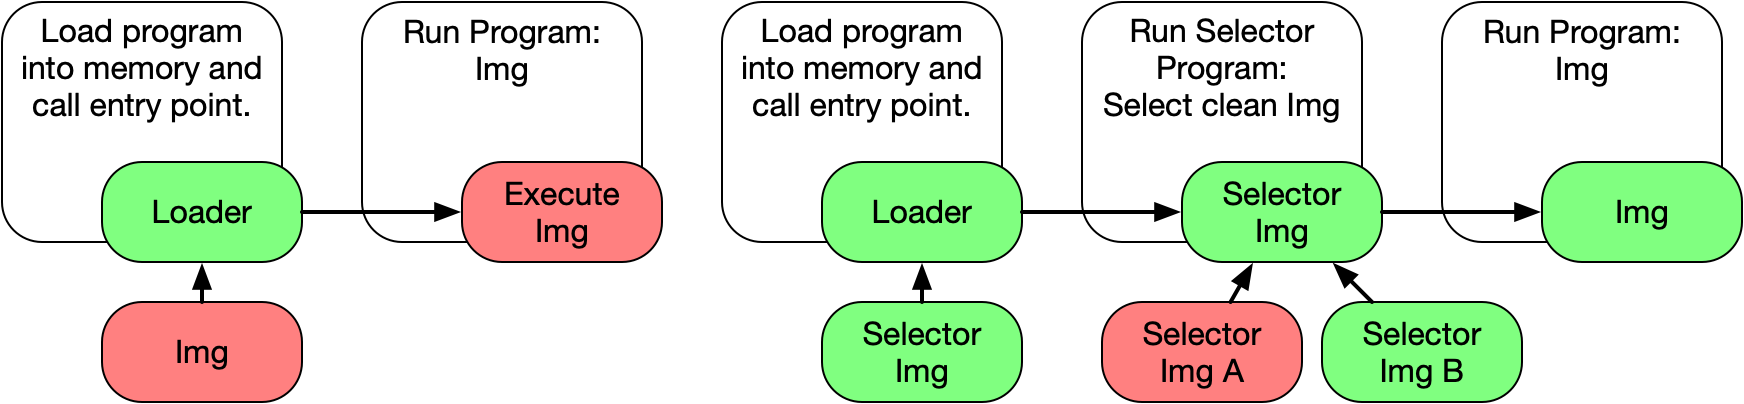
\includegraphics[width=\linewidth]{Chapter-6/figs/rlcr-sequence.png}
  \caption{RLCR execution sequence.
           The loader initializes the system, validates available images (single- or dual-image configurations),
           and transfers control to the first valid region.}
  \label{fig:rlcr-seq}
\end{figure}

\section{Evaluation Setup}
RLCR is evaluated using a dual-image configuration in which two identical program regions share the same total redundancy capacity used in later schemes.
Fault injection introduces persistent errors into non-volatile memory to emulate realistic corruption scenarios.
At startup, the validation routine performs integrity checks and selects the first valid image.
The following measurements are collected:
\begin{itemize}
  \item \textbf{Survivability:} probability that at least one region remains valid after fault injection.
  \item \textbf{Startup latency:} time required for integrity checks and region selection.
  \item \textbf{Memory overhead:} total space occupied by the replicated images.
\end{itemize}
This baseline establishes a reference against which finer-granularity replication methods will be compared in later chapters.

\section{Results}
Experiments confirm that RLCR maintains correct execution whenever at least one region validates successfully.
Since all runtime control flow occurs within the selected image, execution behavior after selection matches that of a non-replicated program.
Validation time scales with region size, and survivability follows the probabilistic model defined earlier as a function of region capacity ($R$) and replication count ($N$).
These results provide the foundation for understanding how finer-granularity approaches refine fault containment while preserving the same total redundancy capacity.

\section{Limit Study (Placeholder)}
\label{sec:rlcr-limit-study}
This section will present the limit study for Region-Level Code Replication once experimental data becomes available.
It will follow the same structure as the \emph{Repair Limit Study}, including:
\begin{itemize}
  \item Experimental configuration and parameters (e.g., number of replicated regions, fault injection rate, validation granularity).
  \item Quantitative results showing survivability and system startup cost as functions of redundancy and fault density.
  \item Comparative discussion of observed saturation points, where additional redundancy yields diminishing returns.
\end{itemize}
At this stage, the section serves as a placeholder for the forthcoming data analysis and figures.

\section{Summary}
RLCR duplicates complete program regions, verifies them at startup, and selects one region for execution.
After selection, control flow is direct and unmodified within the chosen region; no runtime redirection is required.
This chapter establishes the baseline for subsequent techniques---Function-Level and Basic-Block-Level replication---which introduce runtime redirection at progressively finer points in the control flow while keeping overall redundancy storage constant.
% ---------------------------------------------------
\chapter{Function-Level Code Replication (FLCR)}
\label{chap:flcr}
% ---------------------------------------------------

\section{Overview}
Function-Level Code Replication (FLCR) divides a program into individually replicated functions.
Each function maintains one or more redundant copies within the same total redundancy capacity
as region-level replication. At runtime, each replica is validated, and all function calls are
redirected through a runtime indirection layer to a verified target.
This introduces runtime indirection at function boundaries while maintaining normal control flow
inside each function body once execution begins.

% ---------------------------------------------------
\section{Mechanism}
FLCR introduces runtime redirection at function boundaries through a coordinated set of metadata
structures and control components that manage validation, selection, and indirection.
During compilation, each function call—whether direct or indirect—is rewritten to pass through
an indirection layer that dynamically resolves the target at runtime.
This ensures that every control transfer passes through a verification-aware interface,
maintaining consistent access to valid targets.

\subsection{Static Metadata}
Static metadata defines the structure and integrity information for all function replicas.
It is generated in two stages: partially at compile time and completed at post-link time once
code layout and binary contents are finalized.

\begin{itemize}
  \item \textbf{Function Address Table:}
        Generated at compile time. Lists the base address of every function replica so the
        runtime can locate and identify each function.
  \item \textbf{Function Size Table:}
        Generated at post-link time. Records the exact compiled size of each function replica,
        enabling accurate boundary identification for hash computation.
  \item \textbf{Function Hash Table:}
        Generated at post-link time. Stores the precomputed hash for each function replica.
        During execution, the validator recomputes these hashes to confirm integrity.
\end{itemize}

\subsection{Runtime Dynamic Data}
Dynamic metadata represents the current runtime state of all protected functions and is
updated during initialization.

\begin{itemize}
  \item \textbf{Indirection Table (ITab):}
        A fixed-size array indexed by function identifier.
        Each entry contains a pointer to the currently validated target.
        ITab supports all \textbf{direct calls}, where the function index is statically known.
  \item \textbf{Indirection Map (IMap):}
        A binary-searchable map sorted by function address.
        It contains entries for \textbf{all protected functions}, associating each original
        function address with its validated target.
        The IMap supports \textbf{indirect calls} (via function pointers or callbacks)
        and serves as the central reference structure for runtime validation and lookup.
        Its sorted layout allows deterministic binary search without dynamic allocation or hashing.
\end{itemize}

\subsection{Core Components}
\begin{itemize}
  \item \textbf{Validator:}
        Computes the hash for each function replica using the Function Address, Size, and Hash tables.
        Marks replicas as valid if the computed hash matches the expected reference value.

  \item \textbf{Selector:}
        Invokes the Validator to verify all function replicas and determine valid targets.
        If no valid replica exists, the Selector falls back to the first replica in the set.

  \item \textbf{Metadata Initializer:}
        Calls the Selector at startup and uses its results to populate all runtime dynamic structures.
        It writes the validated targets into ITab and IMap, initializes validation states,
        and finalizes all data structures for runtime access.

  \item \textbf{Indirect Resolver:}
        Executes only at \textbf{call sites that were originally indirect}, such as function pointers
        or callbacks. It searches the IMap for the entry corresponding to the original function
        address and retrieves the validated target before control transfer.
\end{itemize}

\subsection{Call-Site Transformation}
FLCR rewrites every function invocation to pass through an indirection layer that resolves
the callee to a validated target at runtime.
Two transformations are applied depending on whether the original call target is static or dynamic.

\begin{table}[h!]
  \centering
  \renewcommand{\arraystretch}{1.2}
  \begin{tabularx}{\linewidth}{|l|X|X|}
    \hline
    \textbf{Call Type} & \textbf{Original} & \textbf{Transformed} \\ \hline
    Direct call   & \texttt{call foo()} & \texttt{target ← ITab[FID\_foo]} → \texttt{call target()} \\ \hline
    Indirect call & \texttt{fptr()}     & \texttt{target ← resolver(fptr)} → \texttt{call target()} \\ \hline
  \end{tabularx}
  \caption{FLCR call-site transformation for direct and indirect calls.}
  \label{tab:flcr-callsite}
\end{table}

\textbf{Description:}
\begin{itemize}
  \item \textbf{Direct calls:}
        Each static call site is assigned a compile-time function identifier (FID).
        At runtime, the call retrieves its validated target from the Indirection Table (ITab)
        before execution.
  \item \textbf{Indirect calls:}
        Calls made through function pointers or callbacks are passed to the \textit{resolver},
        which performs a binary search on the Indirection Map (IMap) to locate the validated
        target corresponding to the original function address.
\end{itemize}

All function invocations—direct or indirect—therefore pass through the same validation-aware
indirection layer, ensuring that execution always targets verified code.

% ---------------------------------------------------
\section{Execution Flow}
At runtime, control first reaches the internal entry point \texttt{\_Entry}, which immediately
invokes the \textbf{Metadata Initializer} before transferring control to the validated
program entry replica (\texttt{Entry.1}).
The initializer calls the \textbf{Selector}, which in turn invokes the \textbf{Validator}
to verify all function replicas and identify valid targets.
Once validation is complete, the runtime indirection structures (\texttt{ITab} and
\texttt{IMap}) are populated so that subsequent execution proceeds entirely through
verified targets.

Figure~\ref{fig:baseline-sequence} shows a baseline execution sequence without replication,
where function calls occur as intended.
Figure~\ref{fig:flcr-sequence} illustrates the FLCR sequence,
where \texttt{\_Entry} and the \textbf{Metadata Initializer} together form a
startup trampoline that redirects control to the validated entry target.

\begin{enumerate}
  \item \textbf{\_Entry:} The trampoline entry point that calls the
        \textbf{Metadata Initializer} and then jumps to the validated \texttt{Entry.1} target.
  \item \textbf{Metadata Initialization:} Invokes the \textbf{Selector}, which calls the
        \textbf{Validator} to compute hashes and determine valid replicas for each function.
  \item \textbf{Runtime Structure Setup:} The Selector provides validated targets to the
        \textbf{Metadata Initializer}, which writes them into \texttt{ITab} and \texttt{IMap},
        finalizing the runtime data structures.
  \item \textbf{Entry.1 (Validated Entry):} Normal execution begins from the validated
        entry function. Direct calls fetch targets from \texttt{ITab};
        indirect calls use the \textbf{resolver} to look up targets in \texttt{IMap}.
\end{enumerate}

This startup sequence ensures that every function call—direct or indirect—is routed through
validated metadata and that all control-flow transitions occur within verified code regions.

\begin{figure}[t]
  \centering
  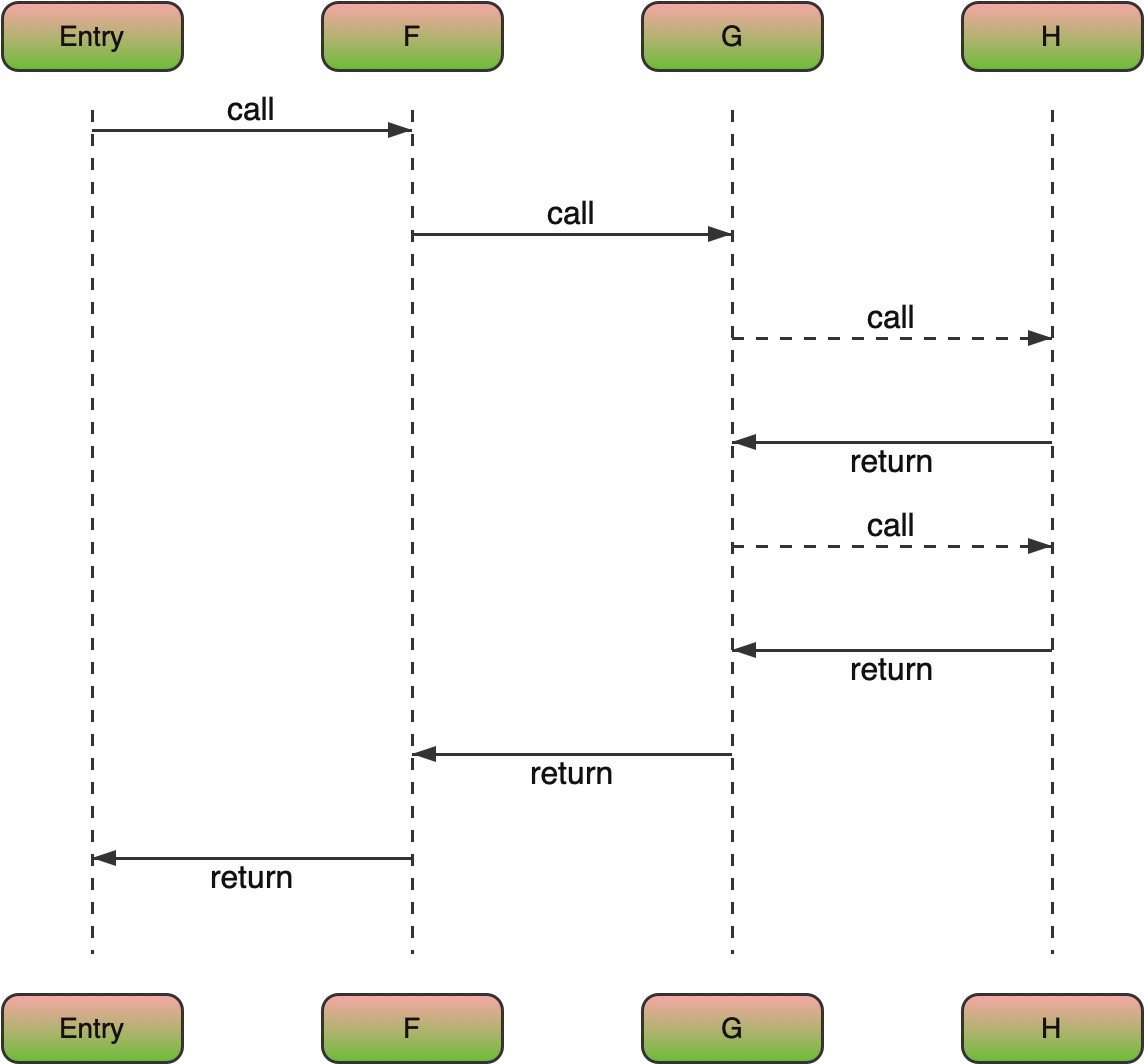
\includegraphics[width=0.9\linewidth]{Chapter-7/figs/baseline-sequence.png}
  \caption{Baseline execution sequence without replication or indirection.
           Function calls occur directly between functions without validation.}
  \label{fig:baseline-sequence}
\end{figure}

\begin{figure}[t]
  \centering
  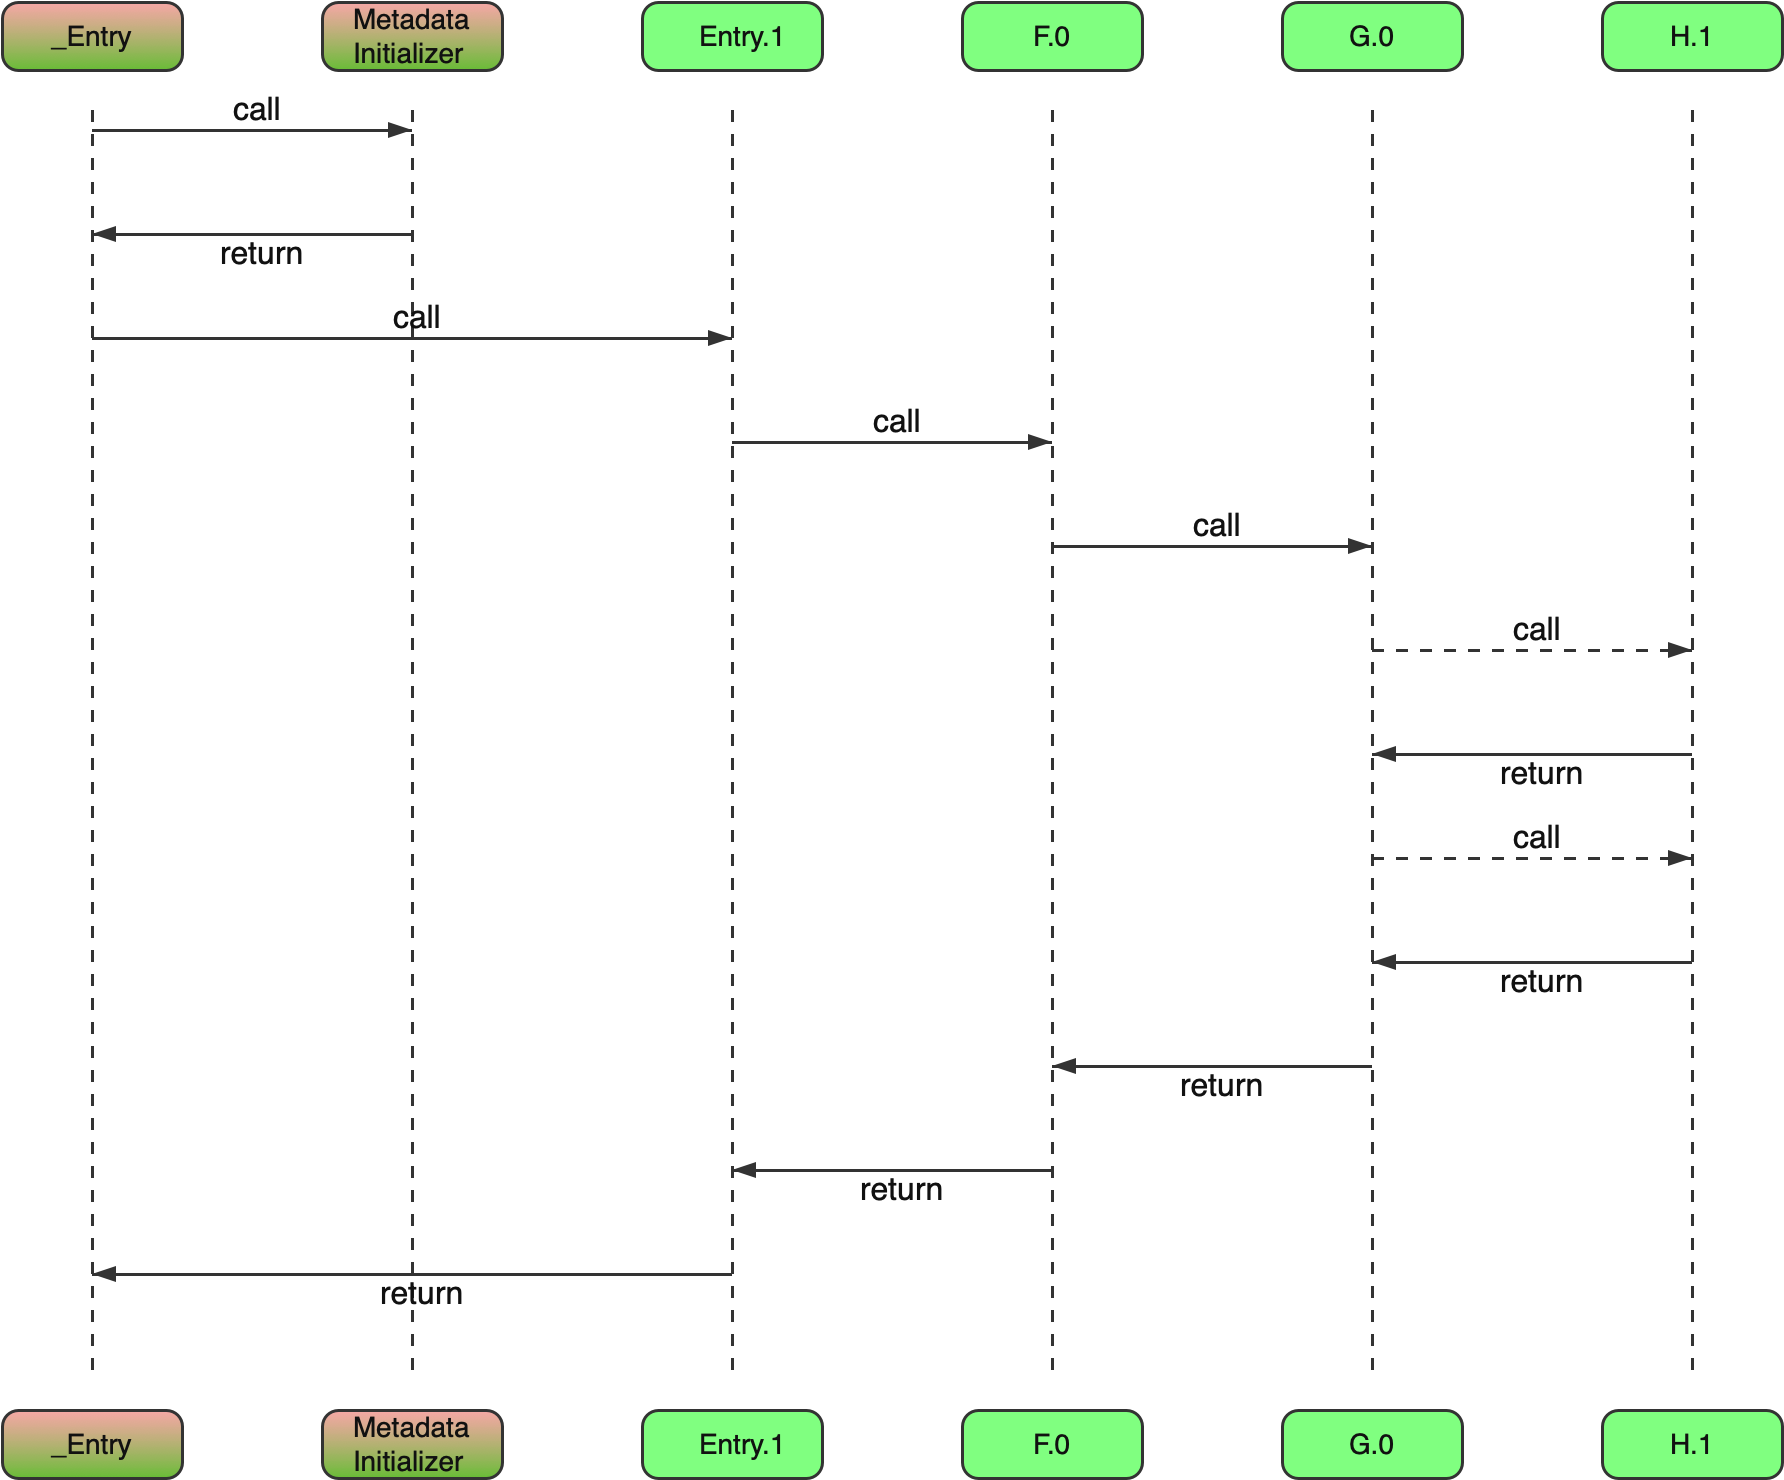
\includegraphics[width=0.9\linewidth]{Chapter-7/figs/flcr-sequence.png}
  \caption{Execution flow under FLCR. The internal \texttt{\_Entry} invokes the
           \textbf{Metadata Initializer}, which calls the \textbf{Selector} to validate and
           populate runtime structures. Control then transfers to the validated
           \texttt{Entry.1} target, after which all calls proceed through validated indirection.}
  \label{fig:flcr-sequence}
\end{figure}

% ---------------------------------------------------
\section{Limit Study}
The following limit study evaluates Function-Level Code Replication (FLCR) under controlled
fault injection to determine its reliability across a range of redundancy configurations.
This study uses the same experimental framework and methodology established for the
baseline and region-level replication (RLCR) analyses.

\subsection{Setup}
Each benchmark is configured to use the same total amount of redundant storage as in
the region-level experiments, but the replicas are distributed across individual functions
rather than entire code regions.
The fault injection method follows the same procedure as the baseline:
random bit flips are introduced directly into the program image while excluding shared
library functions and read-only data sections (\texttt{.data} and \texttt{.rodata}).
All injected faults are constrained to user-level executable regions to isolate the
impact of code corruption.

Each experiment executes 1,000 randomized trials per fault rate.
The primary metric measured is:
\begin{itemize}
  \item \textbf{Reliability:} The probability that all required functions execute
        correctly under a given fault density, measured as the fraction of successful
        program runs.
\end{itemize}

Figure~\ref{fig:flcr-reliability} summarizes observed reliability across fault densities
and compares FLCR with the unprotected baseline and RLCR configurations.

\begin{figure}[t]
  \centering
  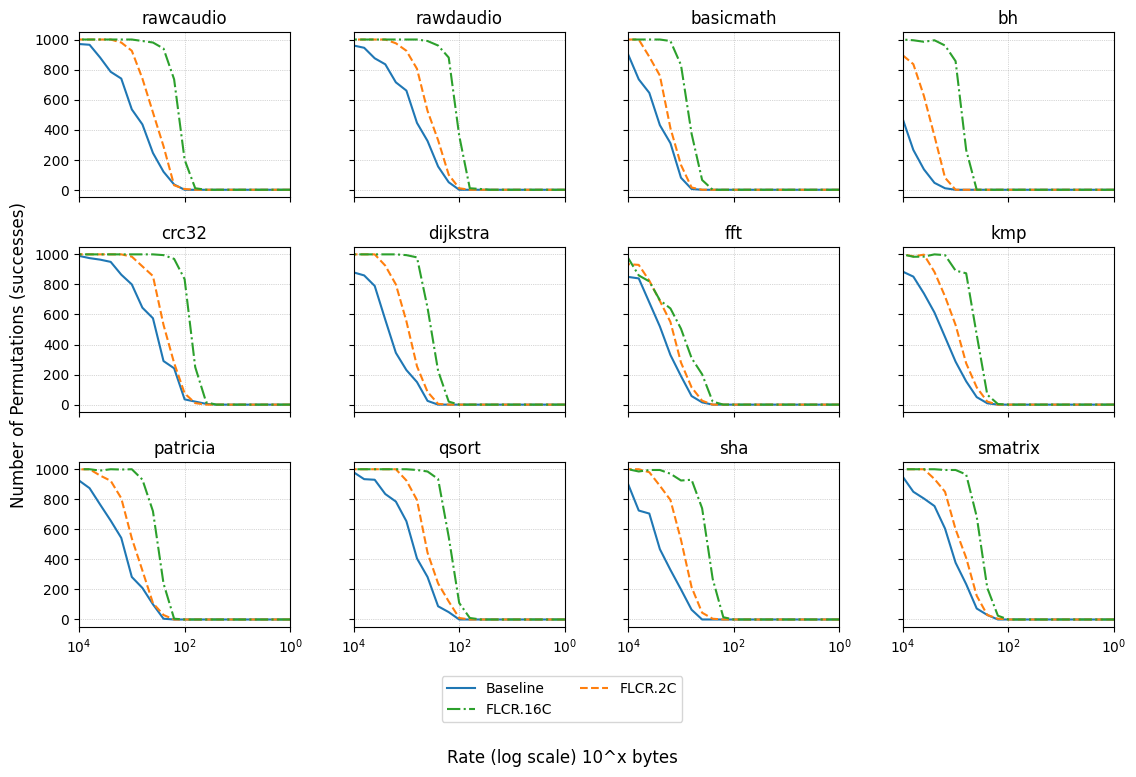
\includegraphics[width=\linewidth]{Chapter-7/figs/flcr-reliability.png}
  \caption{Reliability of FLCR under increasing fault density compared with baseline
           and RLCR configurations. Each curve represents the fraction of successful
           runs out of 1,000 trials.}
  \label{fig:flcr-reliability}
\end{figure}

\subsection{Results}
FLCR maintains correct execution in cases where region-level replication fails due to
localized corruption. Because each function is independently validated and redirected
through a verified target, faults that affect a single function do not compromise the
entire image. Reliability degrades gradually as fault density increases, reflecting
the probability that all required functions retain at least one valid replica.

\subsection{Interpretation}
These results confirm that distributing redundancy at the function level increases
fault containment and improves overall reliability under equal redundancy capacity.
Where RLCR invalidates an entire region after a single failure, FLCR isolates damage
to individual functions, preserving operational integrity of the remaining code.

The magnitude of improvement varies with the program’s function-size profile.
Benchmarks with many small functions benefit most, since localized faults are unlikely to
simultaneously eliminate all replicas of every required function. Conversely, workloads
dominated by a few large functions exhibit sharper reliability drop-offs because a single
faulted hot function removes a larger fraction of the effective code base.

\begin{figure}[t]
  \centering
  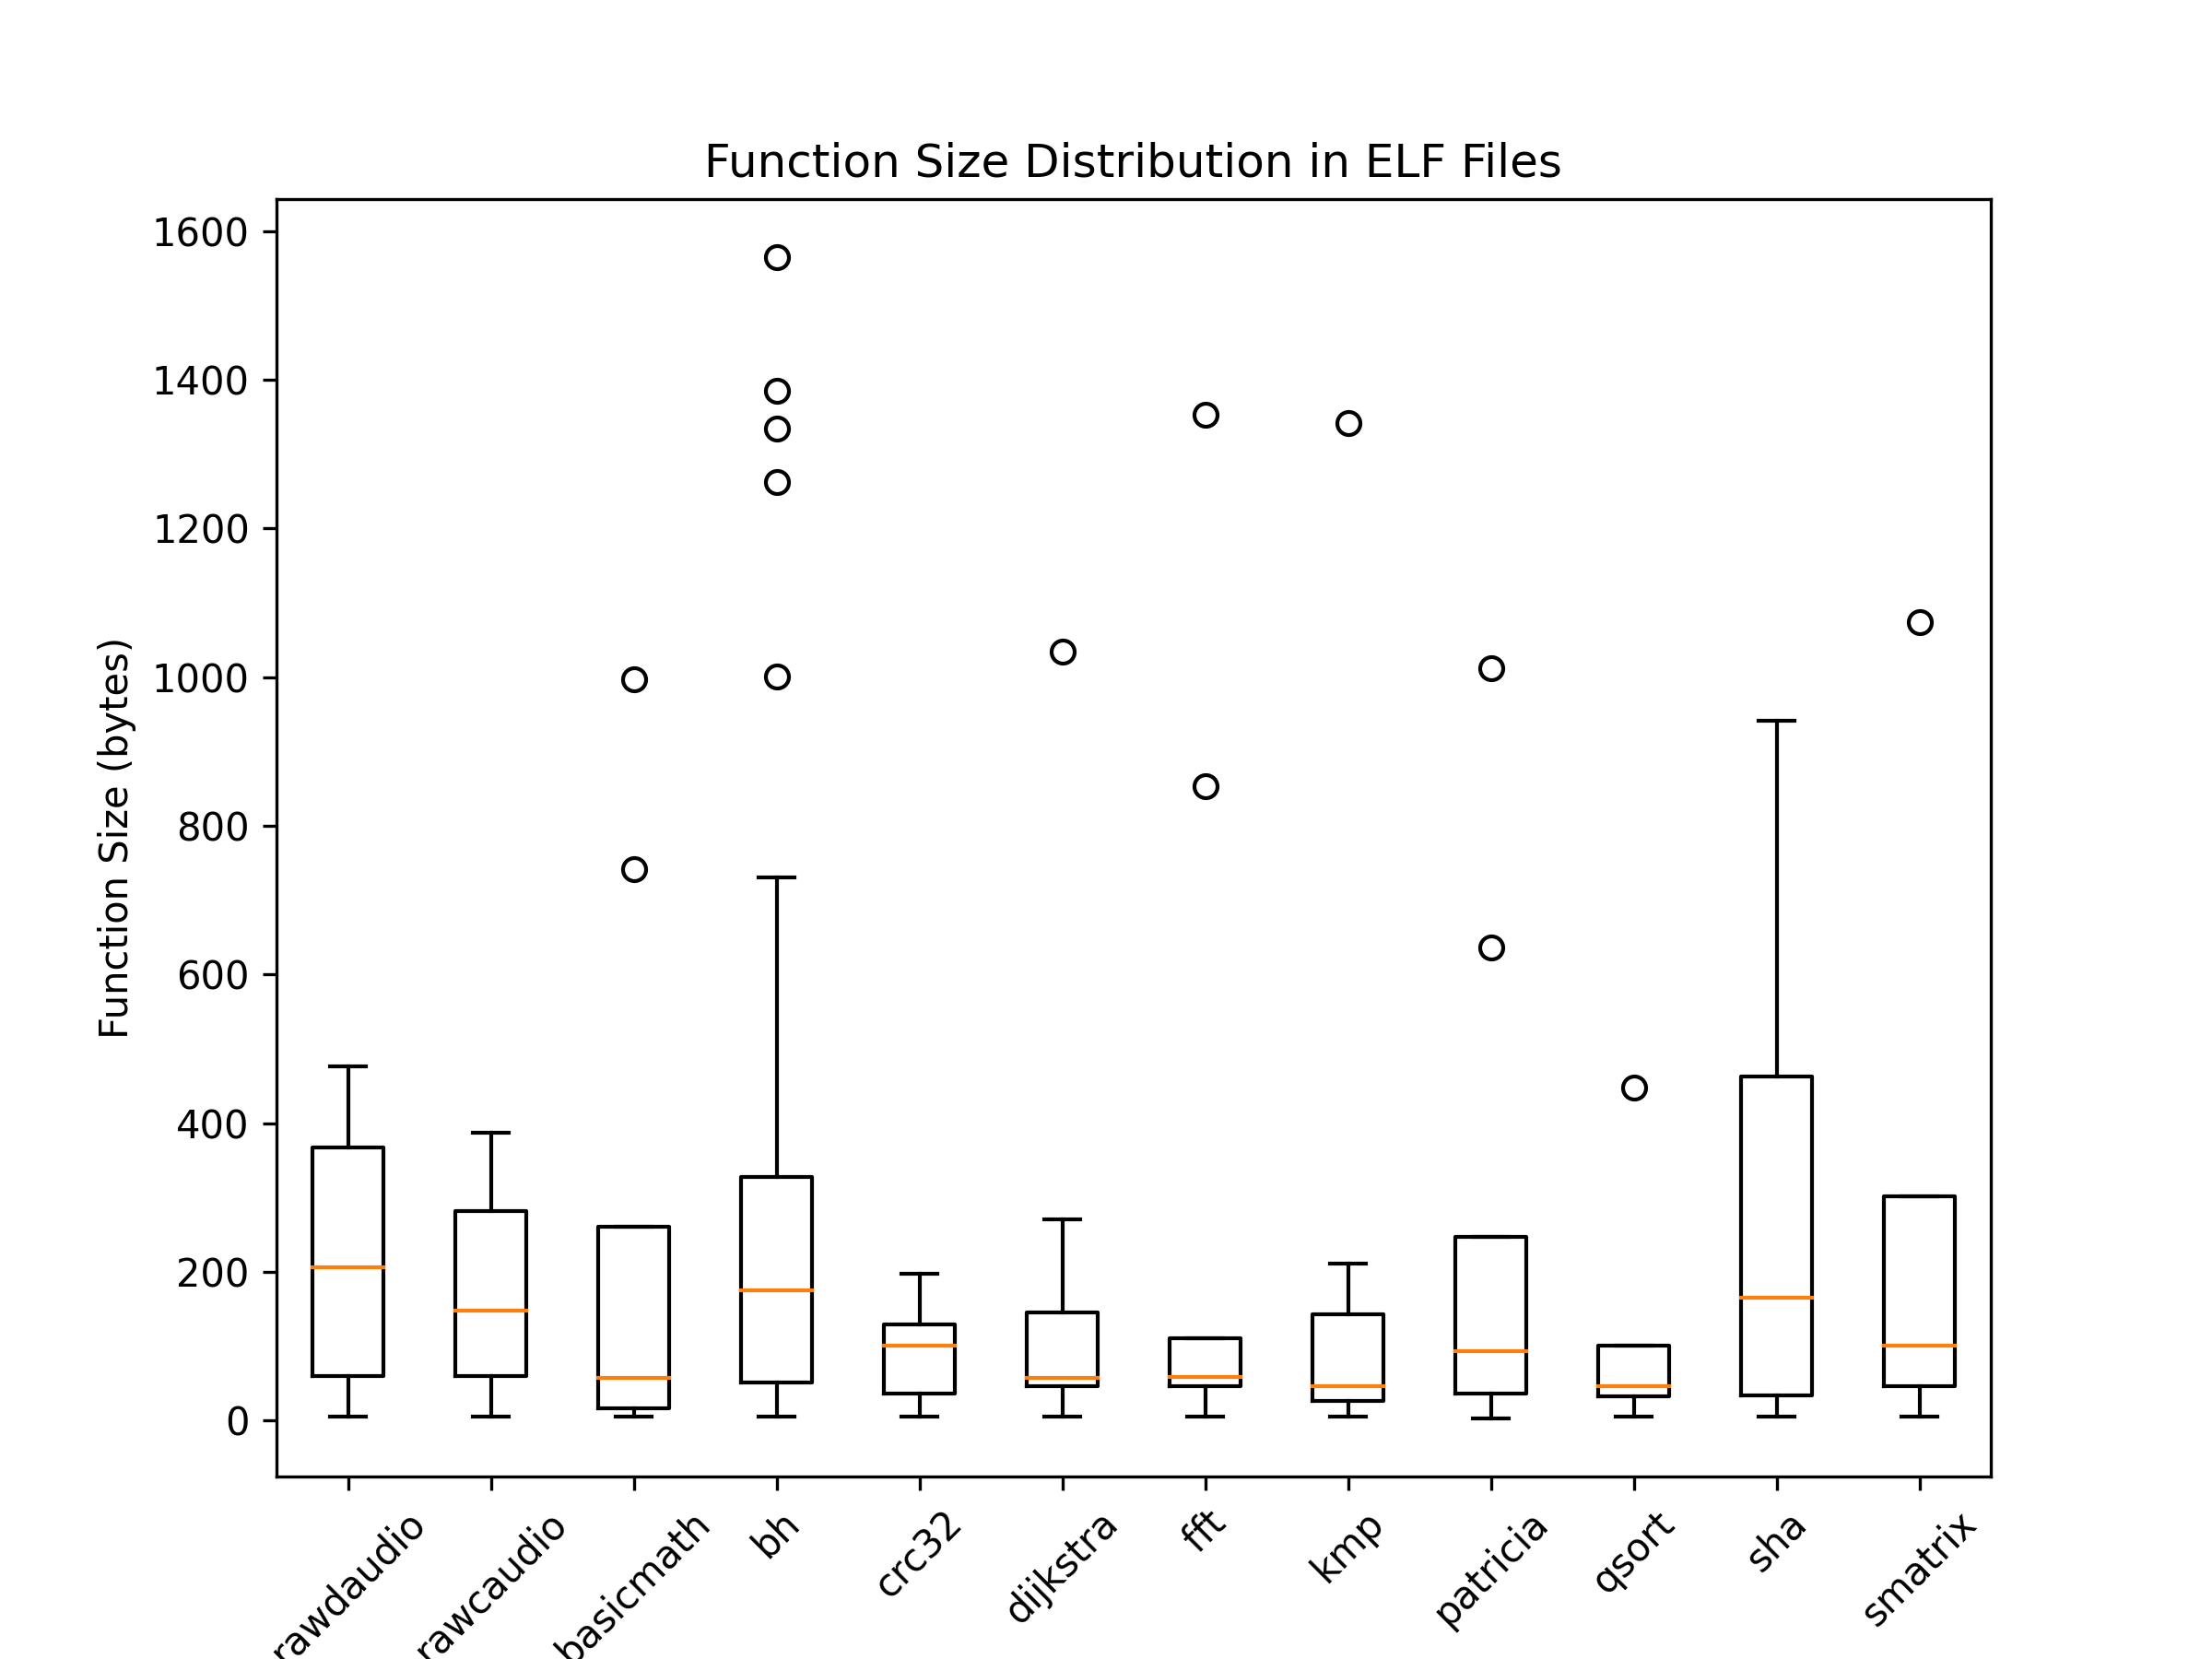
\includegraphics[width=0.9\linewidth]{Chapter-7/figs/size-profile.png}
  \caption{Per-benchmark distribution of function sizes (bytes). Each box summarizes the
           interquartile range with median (orange line); markers indicate outliers.
           Size heterogeneity explains variation in FLCR reliability improvements:
           many small functions favor higher survivability; a few large functions reduce it.}
  \label{fig:flcr-size-profile}
\end{figure}

The size distributions in Fig.~\ref{fig:flcr-size-profile} help explain cross-benchmark
differences in Fig.~\ref{fig:flcr-reliability}. Benchmarks such as those with tighter,
smaller functions tend to sustain higher success rates under growing fault density, while
benchmarks with heavy-tailed size distributions (large outliers) show earlier saturation.
This suggests two practical guidelines for FLCR deployments: (i) prioritize replication
depth for large, high-centrality functions; and (ii) ensure at least one replica of small,
frequently invoked functions to maximize aggregate reliability.

% ---------------------------------------------------
% ---------------------------------------------------
\section{Summary}
Function-Level Code Replication (FLCR) extends runtime fault tolerance by introducing
indirection at the level of function calls. Each function is validated independently,
and all invocations—direct or indirect—are redirected through the ITab or IMap to
their verified targets. This design maintains execution continuity even when individual
functions are corrupted, offering finer-grained fault isolation than region-level
replication (RLCR) under the same redundancy capacity.

However, the reliability improvement of FLCR depends strongly on the distribution of
function sizes within the program. As shown in Fig.~\ref{fig:flcr-size-profile},
benchmarks with many small, evenly sized functions exhibit much higher survivability
than those dominated by large functions. Equalizing function size across an entire
program is not straightforward, since compiler optimizations and control-flow structures
naturally produce functions of varying length and complexity.

Achieving a uniform replication granularity becomes more practical at the next level
of abstraction—\textbf{Basic-Block-Level Code Replication (BBLCR)}—where code is divided
into control-flow blocks of comparable size. BBLCR thus provides a more consistent basis
for balancing replication cost and fault coverage, extending FLCR’s principles into the
instruction path itself.
% ---------------------------------------------------
\chapter{Basic-Block-Level Code Replication (BBLCR)}
\label{chap:bblcr}
% ---------------------------------------------------

\section*{Overview}
Basic-Block-Level Code Replication (BBLCR) refines the principles of FLCR by moving
validation and redirection from function boundaries down to individual control-flow blocks.
Each basic block—defined as a straight-line sequence of instructions ending in a branch or jump—
is treated as an independently verifiable unit.  If a fault corrupts one block, execution can
skip over the damaged block and continue using a valid counterpart instead of discarding the
entire function.

While FLCR isolates faults between functions, BBLCR extends that protection inside functions,
enabling the program to survive corruption at a much finer granularity.

% ---------------------------------------------------
\section*{Mechanism}
BBLCR introduces runtime validation and redirection for intra-function control flow.
Every branch or jump instruction is rewritten so that its destination is resolved through
a runtime lookup structure known as the \textbf{Block Table (BTab)}, which records the
currently validated address of each replicated basic block.
This structure performs the same role as the ITab in FLCR but operates one level deeper.

\subsection*{Static Metadata}
Static metadata describes all replicated basic blocks and is finalized after linking,
when instruction addresses and block boundaries are fully known.

\begin{itemize}
  \item \textbf{Block Address Table:} lists the base address of every block replica within each function.
  \item \textbf{Block Size Table:} records the byte length of each block, used for hash computation.
  \item \textbf{Block Hash Table:} contains reference checksums for every replica, generated after linking and relocation.
\end{itemize}

\subsection*{Runtime Dynamic Data}
At runtime, two structures maintain the validated execution state:

\begin{itemize}
  \item \textbf{Block Table (BTab):} maps each block identifier (BID) to its validated target.
        All conditional and unconditional branches resolve through this table.
  \item \textbf{Branch Map (BMap):} used for indirect or computed jumps; associates the original
        target address with the verified replica.  It supports control transfers that are not statically known.
\end{itemize}

\subsection*{Core Components}
BBLCR reuses the same validation framework as FLCR but applies it at the basic-block level.

\begin{itemize}
  \item \textbf{Validator:} computes and checks the hash of every basic-block replica.
  \item \textbf{Selector:} chooses a valid replica for each block; if none are valid, it defaults to the first replica.
  \item \textbf{Metadata Initializer:} runs once at startup, invoking the Selector and Validator to populate BTab and BMap.
  \item \textbf{Edge Resolver:} executes only at runtime branch sites that were originally indirect or computed jumps,
        searching BMap for the validated target.
\end{itemize}

\subsection*{Branch Transformation}
Every branch and jump instruction is rewritten to route through the runtime indirection
layer, ensuring that all control flow enters only validated basic blocks.
Each transformation consults the \textbf{Block Table (BTab)} for statically known edges,
or the \textbf{Branch Map (BMap)} for computed or indirect edges.

\begin{table}[h!]
  \centering
  \renewcommand{\arraystretch}{1.2}
  \begin{tabularx}{\linewidth}{|l|X|X|}
    \hline
    \textbf{Branch Type} & \textbf{Original} & \textbf{Transformed} \\ \hline
    Unconditional branch &
    \texttt{jmp L1} &
    \texttt{load target ← BTab[BID\_L1]} \newline
    \texttt{jmp target} \\ \hline

    Unconditional branch (indirect) &
    \texttt{jmp *ptr} &
    \texttt{target ← resolver(ptr)} \newline
    \texttt{jmp target} \\ \hline

    Conditional branch &
    \texttt{br cond, L\_T, L\_F} &
    \texttt{load T ← BTab[BID\_T]} \newline
    \texttt{load F ← BTab[BID\_F]} \newline
    \texttt{sel target ← cond ? T : F} \newline
    \texttt{br target} \\ \hline

    Conditional branch (indirect) &
    \texttt{br cond, *ptr\_T, *ptr\_F} &
    \texttt{T ← resolver(ptr\_T)} \newline
    \texttt{F ← resolver(ptr\_F)} \newline
    \texttt{sel target ← cond ? T : F} \newline
    \texttt{br target} \\ \hline
  \end{tabularx}
  \caption{Unified BBLCR branch transformation for unconditional, conditional,
           and indirect control transfers.}
  \label{tab:bblcr-transform}
\end{table}

This unified transformation guarantees that all control-flow edges—direct, conditional,
and indirect—are redirected through validated structures.
Because basic blocks are smaller than functions, faults can be contained more precisely,
allowing recovery within individual routines.

These transformations rely on the presence of \textbf{indirect branch instructions}
within the instruction set architecture.
Such instructions (e.g., ARM \texttt{BX}, RISC-V \texttt{JALR}, x86 \texttt{jmp *reg})
allow branch destinations to be computed dynamically at runtime, enabling seamless
redirection to validated replicas while preserving the original control-flow structure.

Architectures that lack indirect branching (for example, those that only permit fixed
or PC-relative targets) must emulate this behavior using additional control logic.
In such systems, the compiler introduces explicit control or dispatcher blocks,
as described in the next section.

% ---------------------------------------------------
\subsection*{Control and Target Blocks (Systems Without Indirect Branch Support)}
The control and target block distinction arises only on architectures that \emph{lack}
native indirect branch instructions.  In these systems, branches and jumps cannot take
a computed destination directly, so BBLCR must emulate redirection through additional
control logic.

Under such conditions, each original basic block divides into two roles:

\begin{itemize}
  \item \textbf{Target blocks:} contain the executable program logic and act as the true
        branch destinations under validation.
  \item \textbf{Control blocks:} inserted to perform runtime redirection and validation
        lookups through the \textbf{BTab} or \textbf{BMap} structures.
\end{itemize}

Whenever a target block is replicated, a control block must precede it to handle redirection.
If that control block later becomes the target of another branch, an additional control
block must be introduced in front of it—creating recursive expansion and increasing
control-block density.  This expansion raises instruction count and weakens spatial locality
between related code regions.

Ideally, a target block and its associated control block would remain \textbf{contiguous in memory},
forming a small, self-contained protection region.  In practice, compiler scheduling, padding,
and link-time reordering scatter these blocks throughout the binary, making contiguity rare.
Target and control blocks often become \textbf{discontinuous}, preventing validation as a single region.

Because of this discontinuity, it becomes impossible to maintain \textbf{block groups}—sets of
related blocks that could be invalidated together if one fails validation.  Inserted control
stubs fragment the layout, separating targets that once shared a logical flow.  Group invalidation
therefore becomes unsafe, since invalidating a ``group'' might also remove unrelated control code.

Consequently, protection boundaries must terminate at the \textbf{target block}.
The control block functions as a trusted redirector but cannot itself be validated in the same way,
as its position and linkage may vary across compilations.  Only the target block can be considered
clean and fault-free under the validation model.

This structural limitation highlights a key tradeoff of fine-grained replication:
as granularity increases, isolation improves, but on systems without indirect branch support,
compiler layout and control fragmentation make contiguous protection increasingly difficult.

% ---------------------------------------------------
\section*{Control-Flow Structure and Replication}
The structure of BBLCR can be illustrated using the simple loop example shown in
Figure~\ref{fig:bblcr-combined}.
Subfigure~(a) depicts the baseline control-flow graph of a typical \texttt{for} loop,
composed of five basic blocks: \textbf{Entry}, \textbf{Condition}, \textbf{Body},
\textbf{Increment}, and \textbf{Exit}. Control flows cyclically between the
\textbf{Condition} and \textbf{Body} blocks until the loop terminates.

Subfigure~(b) shows the same loop after transformation under BBLCR.
Each basic block is independently replicated, and all control-flow edges are redirected
through the validated \textbf{Block Table (BTab)}.
Conditional branches dynamically resolve both their true and false targets through BTab,
ensuring that every transition occurs only between verified replicas.

\begin{figure}[t]
  \centering
  \begin{subfigure}[t]{0.47\linewidth}
    \centering
    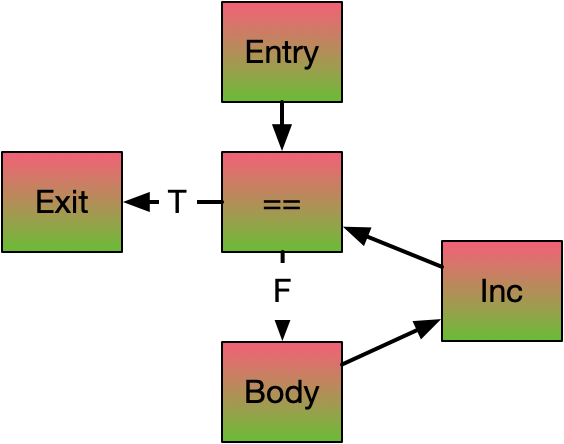
\includegraphics[width=\linewidth]{Chapter-8/figs/bblcr-baseline.png}
    \caption{Baseline control-flow graph for a simple \texttt{for} loop showing
             \textbf{Entry}, \textbf{Condition}, \textbf{Body}, \textbf{Increment},
             and \textbf{Exit} blocks.}
    \label{fig:bblcr-baseline}
  \end{subfigure}
  \hfill
  \begin{subfigure}[t]{0.47\linewidth}
    \centering
    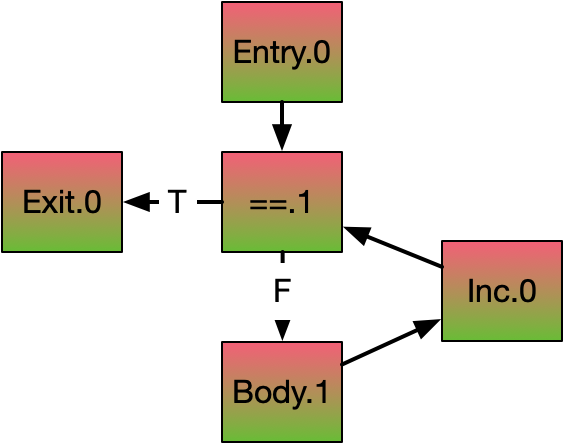
\includegraphics[width=\linewidth]{Chapter-8/figs/bblcr-replicated.png}
    \caption{Replicated control-flow graph under BBLCR. Each branch and jump resolves
             through the validated \textbf{BTab}, allowing the system to skip corrupted
             basic blocks and continue through verified replicas.}
    \label{fig:bblcr-replicated}
  \end{subfigure}
  \caption{Comparison of baseline and BBLCR-transformed control flow for a simple loop:
           (a) baseline function layout, (b) replicated layout with runtime redirection.}
  \label{fig:bblcr-combined}
\end{figure}

This combined view highlights two central aspects of BBLCR:
\begin{enumerate}
  \item \textbf{Granularity:} validation occurs at each basic-block boundary,
        allowing localized fault containment within a function.
  \item \textbf{Edge indirection:} every branch and jump is resolved through runtime
        tables, preventing entry into unvalidated code.
\end{enumerate}

In larger applications, each basic block operates as a relocatable unit of verified logic,
connected through fault-tolerant control edges that maintain functional continuity
even in the presence of localized corruption.

% ---------------------------------------------------
\section*{Execution Flow}
At runtime, initialization proceeds identically to FLCR.
The \textbf{Metadata Initializer} invokes the \textbf{Selector} and \textbf{Validator}
to populate the \textbf{BTab} and \textbf{BMap} before execution begins.
After initialization, every intra-function branch and jump passes through the validated indirection layer.

In a baseline program, branches connect directly between blocks with no runtime validation.
Under BBLCR, each branch or jump first consults \textbf{BTab} (for static edges)
or \textbf{BMap} (for computed targets) before transferring control.
This design allows the program to skip corrupted paths dynamically while continuing
through validated replicas.

% ---------------------------------------------------
\section*{Limit Study}
The Basic-Block-Level Code Replication (BBLCR) limit study evaluates the practical
benefits of fine-grained replication in a controlled, minimal environment.
Unlike previous large-scale benchmark studies, this experiment isolates a single
loop construct to observe the effects of corruption and recovery in detail.

\subsection*{Setup}
Figure~\ref{fig:bblcr-limit-flow} illustrates the experimental flow.
A shared library containing a simple \texttt{for}-loop function was used as the test
subject.  The library was independently instrumented for three configurations:
\textbf{Baseline}, \textbf{FLCR}, and \textbf{BBLCR}.

Bit-flip faults were randomly injected into the library’s executable image to
simulate instruction corruption.  The corrupted shared object was then dynamically
loaded and executed by a host program.  During execution, the selection and validation
routines (when enabled) verified and redirected control to validated replicas.
Program output was compared against a known reference output to determine whether
execution remained correct.

\begin{figure}[t]
  \centering
  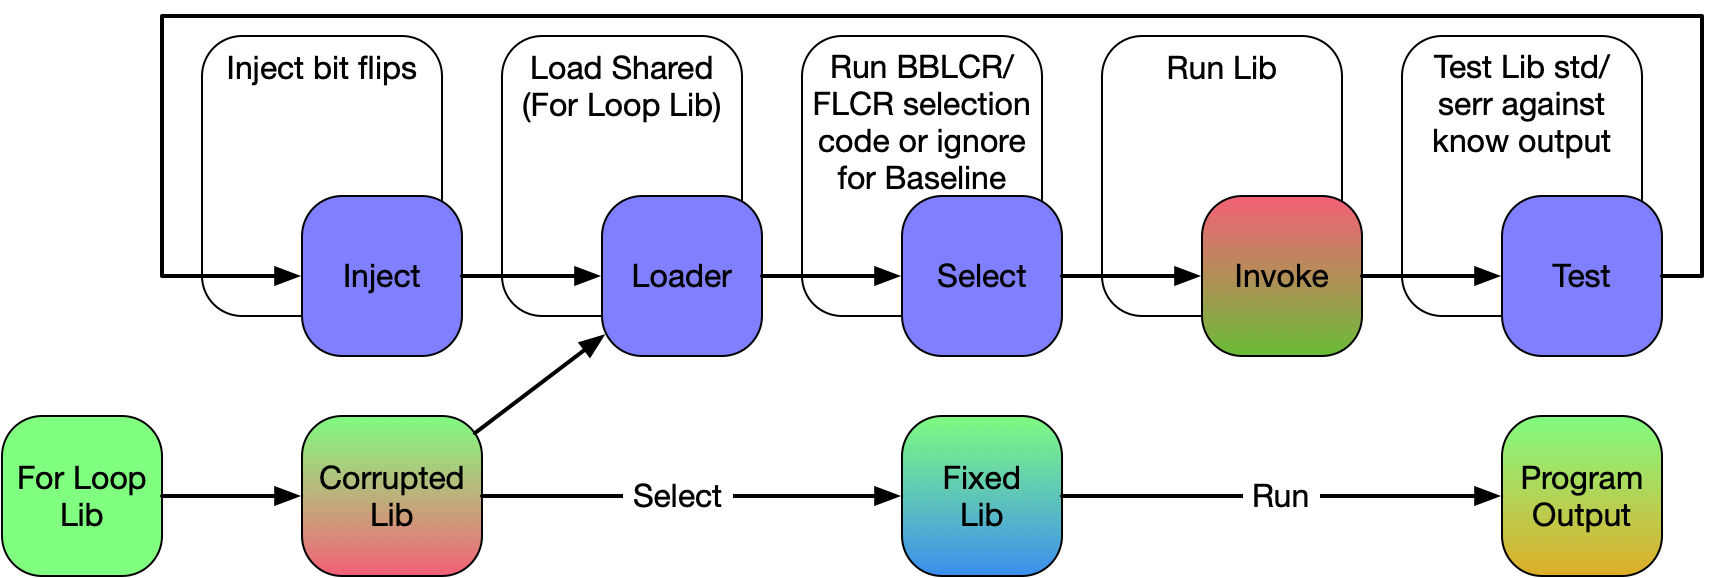
\includegraphics[width=\linewidth]{Chapter-8/figs/bblcr-limit-flow.png}
  \caption{Limit study experimental flow for Baseline, FLCR, and BBLCR configurations.
           A shared library implementing a simple \texttt{for}-loop is corrupted,
           dynamically loaded, and executed.  The resulting output is validated
           against a known reference to measure reliability.}
  \label{fig:bblcr-limit-flow}
\end{figure}

\subsection*{Results}
The fault injection campaign was repeated across multiple corruption levels,
each representing an increasing density of random bit flips within the shared object.
For the \textbf{Baseline}, any corruption within the loop body typically resulted
in immediate program failure or incorrect output.

With \textbf{FLCR}, function-level replication successfully recovered from
corruptions that affected a subset of functions, but failures persisted when
multiple corrupted basic blocks appeared within the same function body.
\textbf{BBLCR} eliminated this limitation by validating and redirecting at the
basic-block level, maintaining correct operation even when isolated loop blocks
were corrupted.

\subsection*{Interpretation}
This experiment demonstrates that fine-grained replication significantly improves
software survivability under instruction faults, even in minimal programs.
BBLCR’s local validation and redirection allow execution to bypass individual
corrupted blocks, providing functional continuity where FLCR and Baseline fail.

However, this improvement comes with increased metadata overhead and runtime
complexity, even in a simple workload.  The benefit therefore depends on the
application domain: systems with compact, time-critical code may favor coarser
granularity, while those demanding resilience at any cost—such as recovery loops
or embedded control kernels—stand to gain the most from BBLCR.

% ---------------------------------------------------
\section*{Summary}
This chapter introduced Basic-Block-Level Code Replication (BBLCR),
a fine-grained replication mechanism that operates at the level of individual
basic blocks. BBLCR extends the concept of runtime indirection from functions
to intra-function control flow, using a per-block lookup structure to
validate and redirect execution at each branch boundary.

The design allows the system to isolate faults within specific control-flow
segments, improving fault survivability compared to both FLCR and Baseline.
Through the loop-based limit study, BBLCR maintained correct operation even
when corruption occurred inside individual loop blocks, demonstrating effective
containment at the basic-block level.

However, finer granularity also introduced practical constraints.
Additional control blocks and validation lookups increased metadata overhead,
and compiler scheduling often scattered related blocks, preventing contiguous
protection regions. Only the target block could be considered truly validated,
while the surrounding control logic remained structurally exposed.

In summary, BBLCR achieves the highest fault isolation among the replication
models but exposes tradeoffs in layout continuity and runtime complexity.
Its results form the final stage of the granularity spectrum explored in this work.
The next chapter revisits all limit study results together, comparing
reliability trends and overhead across RLCR, FLCR, and BBLCR configurations.
% ---------------------------------------------------
\chapter{Limit Studies Discussion: Replication and Repair}
\label{chap:limit-discussion}
% ---------------------------------------------------

\section*{Overview}
This chapter consolidates the findings of all limit studies conducted for both
replication and repair mechanisms.  
The goal is to compare how reliability, overhead, and fault containment scale
across different fault-tolerance strategies and levels of granularity.
Replication mechanisms—Region-Level (RLCR), Function-Level (FLCR), and
Basic-Block-Level (BBLCR)—protect execution through redundancy and redirection.
Repair mechanisms, in contrast, reconstruct corrupted code or data in place,
relying on redundant encoding rather than multiple replicas.

Both methods operate under the same probabilistic framework introduced earlier:
survivability depends on the number of redundant elements, their validation
coverage, and the probability of an undetected fault.  
Together, replication and repair form the foundation of the proposed resilience
hierarchy—replication ensures continuity, while repair restores integrity.

% ---------------------------------------------------
\section*{Comparative Reliability}
The reliability data collected across all configurations reveal consistent
scaling behavior: as replication granularity increases, fault containment
improves and survivability extends to finer levels of program structure.
RLCR provides coarse fault isolation by selecting an entire verified image;
FLCR confines faults to the function level; and BBLCR achieves the highest
containment within individual control-flow blocks.

Repair mechanisms complement this trend by targeting individual instructions or
data words rather than entire structural units.  
Where replication avoids faults through redirection, repair mitigates them
through reconstruction.

\begin{figure}[t]
  \centering
  % \includegraphics[width=\linewidth]{Chapter-9/figs/reliability-trends.png}
  \caption{Placeholder for comparative reliability trends across replication and
           repair models (RLCR, FLCR, BBLCR, and Repair).}
  \label{fig:limit-reliability}
\end{figure}

% ---------------------------------------------------
\section*{Overhead and Structural Tradeoffs}
Replication and repair incur different types of cost.  
Replication introduces \textbf{static overhead} in the form of additional memory
for replicas and metadata structures (e.g., ITab, BTab), as well as
\textbf{dynamic overhead} from validation and redirection at runtime.
Repair mechanisms, meanwhile, add \textbf{computational overhead} for decoding
and reconstruction, especially when error density is high.

As granularity increases—from regions to basic blocks—the validation frequency
rises sharply, increasing both instruction count and runtime latency.
In contrast, repair overhead scales with the number of faults encountered rather
than program structure, making it more predictable in low-fault environments.

\begin{table}[h!]
  \centering
  \renewcommand{\arraystretch}{1.2}
  \begin{tabularx}{\linewidth}{|l|X|X|X|}
    \hline
    \textbf{Mechanism} & \textbf{Static Overhead} & \textbf{Dynamic Overhead} & \textbf{Notes} \\ \hline
    RLCR  & High (replica images) & Low (startup validation) & Coarse isolation \\ \hline
    FLCR  & Moderate (function replicas) & Moderate (call redirection) & Balance of cost and containment \\ \hline
    BBLCR & High (block metadata) & High (branch redirection) & Fine containment, high complexity \\ \hline
    Repair & Low (code parity) & Variable (reconstruction time) & Continuous protection \\ \hline
  \end{tabularx}
  \caption{Placeholder table comparing overhead characteristics for replication and repair mechanisms.}
  \label{tab:limit-overhead}
\end{table}

% ---------------------------------------------------
\section*{Fault Containment and Recovery Scope}
Each technique limits the spatial and temporal propagation of faults differently:
\begin{itemize}
  \item \textbf{RLCR} recovers at the region or image scale by selecting an alternate verified copy.
  \item \textbf{FLCR} confines corruption to individual functions, maintaining program flow through call-site indirection.
  \item \textbf{BBLCR} provides intra-function containment, validating and rerouting control at the level of basic blocks.
  \item \textbf{Repair} operates below these layers, reconstructing individual corrupted instructions or data words.
\end{itemize}

Replication therefore provides discrete containment boundaries, while repair
extends recoverability to the finest possible scale.
The two can operate in tandem—replication preserves execution continuity while
repair restores local integrity—forming a complementary defense structure.

\begin{figure}[t]
  \centering
  % \includegraphics[width=\linewidth]{Chapter-9/figs/containment-scope.png}
  \caption{Placeholder diagram illustrating fault containment scope for replication and repair mechanisms.}
  \label{fig:limit-containment}
\end{figure}

% ---------------------------------------------------
\section*{Combined Model: Repair within Replication}
In practice, replication and repair need not be exclusive.  
A hybrid model can use replication for immediate fault avoidance and repair for
deferred correction.  For example, if a replicated function fails validation, a
repair subsystem could reconstruct its corrupted copy and reintegrate it into
the validated pool.

This cooperative approach enables long-term reliability without unbounded
replication cost.  Replication provides runtime continuity, ensuring the system
always has a valid execution path, while repair reclaims lost replicas,
restoring redundancy over time.

\begin{figure}[t]
  \centering
  % \includegraphics[width=\linewidth]{Chapter-9/figs/hybrid-model.png}
  \caption{Placeholder for conceptual hybrid model showing interaction between replication and repair layers.}
  \label{fig:limit-hybrid}
\end{figure}

% ---------------------------------------------------
\section*{Summary}
The limit studies collectively demonstrate that increasing replication
granularity improves fault containment but at the expense of control complexity
and metadata size.  Repair mechanisms extend resilience beyond these limits by
addressing corruption directly, rather than redirecting around it.

Replication excels at maintaining continuous execution, while repair restores
full program integrity.  Together, they represent complementary dimensions of
software-based fault tolerance—replication for continuity, repair for recovery.

Future chapters will integrate these models under a unified runtime and compiler
framework to balance redundancy, cost, and self-healing capability.
% ---------------------------------------------------
\chapter{FLCR Compiler}
\label{chap:flcr-compiler}
% ---------------------------------------------------

% Toggle for showing the LLVM Pass section (change to \showflcrpassfalse to hide)
\newif\ifshowflcrpass
\showflcrpasstrue

\section*{Overview}
This chapter details the implementation of Function-Level Code Replication (FLCR)
within the compiler framework. The transformation is organized into eight
phases (A–H), followed by runtime initialization of the Replica Selector Table (RST).
Each phase represents a distinct compiler pass responsible for outlining, cloning,
instrumentation, and metadata emission to enable self-validating replicated code.

% ---------------------------------------------------
% ---------------------------------------------------
\section*{Tool Flow}
Figure~\ref{fig:flcr-tool-flow} shows the complete FLCR build pipeline,
from protected source code to a post-linked binary with injected metadata.
This process is designed to integrate cleanly with any LLVM-based toolchain
and uses standard intermediate formats for compatibility with both Clang
and external linkers.

\begin{figure}[t]
  \centering
  % Update to your actual path if needed
  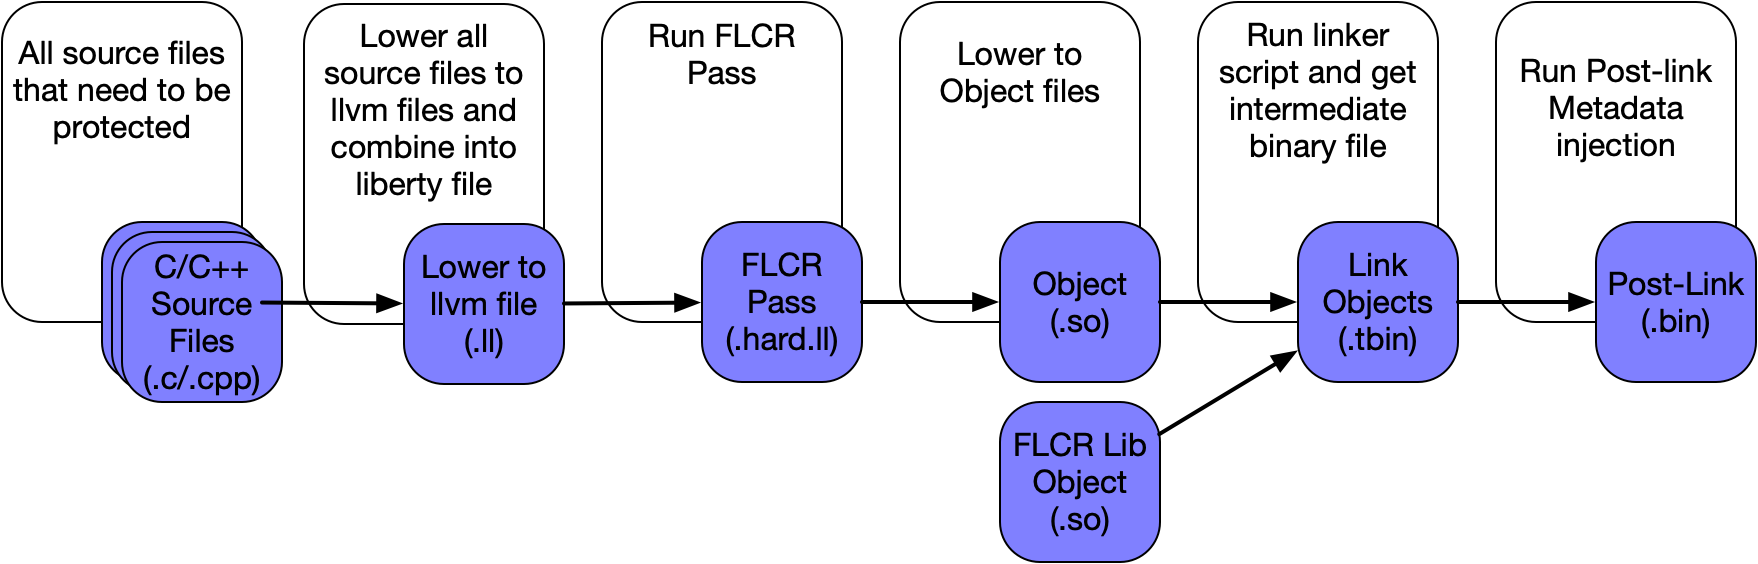
\includegraphics[width=\linewidth]{Chapter-10/figs/flcr-tool-flow.png}
  \caption{FLCR compiler and tool flow. Protected sources are lowered to LLVM IR,
           transformed by the FLCR pass, compiled to objects, linked with the FLCR
           runtime library, and finalized through post-link metadata injection.}
  \label{fig:flcr-tool-flow}
\end{figure}

\paragraph{Stages (left to right).}
\begin{enumerate}
  \item \textbf{Source Collection.}  
        Identify and gather all C/C++ source files that must be protected under FLCR.
        These files form the logical protection unit for the build.
  \item \textbf{IR Generation and Bundling.}  
        Each source is lowered to LLVM IR (\texttt{.ll}) using the standard front end.
        All IR units are then combined into a single IR “library” module for pass execution.
  \item \textbf{Run FLCR Pass.}  
        The FLCR compiler pass transforms the combined IR to insert validation metadata,
        redirection logic, and function clones, producing a hardened module
        (\texttt{.hard.ll}).
  \item \textbf{Lower to Object Files.}  
        The transformed IR is compiled to native object files (\texttt{.o}/\texttt{.so}).
        The FLCR runtime support library is built at this stage as a companion object.
  \item \textbf{Linking.}  
        Application and runtime objects are linked using the standard linker script
        to generate an intermediate binary (\texttt{.tbin}). This step merges all
        function tables and ensures consistent section layout.
  \item \textbf{Post-Link Metadata Injection.}  
        The post-link tool scans the intermediate binary, computes function sizes and
        checksums, and populates the lookup tables emitted by the FLCR pass.
        The final binary (\texttt{.bin}) is fully self-validating.
\end{enumerate}


\paragraph{Artifacts.}
\begin{itemize}
  \item \texttt{*.ll} — per-source LLVM IR files combined into a single library.
  \item \texttt{*.hard.ll} — IR after FLCR pass; includes cloned variants and metadata.
  \item \texttt{*.o}, \texttt{*.so} — compiled objects, including the FLCR runtime object.
  \item \texttt{*.tbin} — intermediate binary prior to metadata injection.
  \item \texttt{*.bin} — final FLCR-protected executable with populated lookup tables.
\end{itemize}


% ---------------------------------------------------
\ifshowflcrpass
  % ---------------------------------------------------
\section*{LLVM Pass}
FLCR is realized as a fixed sequence of compiler passes (A–H). Each pass consumes
IR and/or metadata from the previous step and produces artifacts that the next step
relies on. The table summarizes each phase.

\begin{table}[t]
  \centering
  \renewcommand{\arraystretch}{1.15}
  \begin{tabularx}{\linewidth}{|c|X|X|X|}
    \hline
    \textbf{Phase} & \textbf{Purpose} & \textbf{Key Operations} & \textbf{Primary Outputs} \\ \hline
    A & Entry wrapping & Outline original entry; insert \texttt{code\_init()} and tail-call & New entry thunk; \texttt{.outlined} body \\ \hline
    B & Candidate selection & Apply include/exclude; filter intrinsics/decls; stable order & \textit{Bases}, \textit{BaseIndex} \\ \hline
    C & Indirect resolver & Interpose on function-pointer calls via \texttt{resolve()} & Indirect callsites become resolvable \\ \hline
    D & Clone stubs & Declare \(N\) variants per base (sig/attrs preserved) & \textit{ClonesMap} (stubs) \\ \hline
    E & Globals/metadata & Define lookup, checksums, sizes; set sections; keep alive & \texttt{func\_lookup}, \texttt{func\_checksum}, \texttt{func\_size} \\ \hline
    F & Direct-call rewrite & Replace direct calls to bases with loads from lookup slot & Calls to candidates go via \texttt{func\_lookup[idx]} \\ \hline
    G & Deep clone bodies & Clone base body into each stub; remap SSA & Materialized variant bodies \\ \hline
    H & Catalog/finalize & Build RO address array; optionally drop/keep bases & \texttt{func\_array}; cleaned module \\ \hline
    Runtime & Initialize RST & Validate variants; select first valid; write lookup slot & Populated \texttt{func\_lookup} \\ \hline
  \end{tabularx}
  \caption{Phase purposes, operations, and outputs for the FLCR pass pipeline.}
  \label{tab:flcr-pass-layout}
\end{table}

\clearpage
\subsection*{Phase A — Runtime Initialization Wrapper}
This phase wraps the program’s entry point to integrate the runtime initialization sequence
before any \textbf{hardened user code} executes.
The compiler locates the configured entry function (typically \texttt{main} or another designated symbol)
and outlines its body into a secondary function suffixed with \texttt{.outlined}.
The original entry is reconstructed to first invoke \texttt{code\_init()}—the runtime routine responsible
for preparing FLCR metadata, global tables, and replica structures—before transferring control
to the outlined body.
This guarantees that all fault-tolerance metadata is initialized prior to entering hardened user code,
ensuring that subsequent phases of replication and validation operate on a consistent runtime state.
The outlined entry function is marked for exclusion from later replication stages to avoid
recursive transformation of the bootstrap logic itself.

\begin{algorithm}[H]
\caption{Phase A — Outline Entry and Inject Initialization}
\label{alg:phaseA}
\begin{algorithmic}[1]
\State \textbf{Input:} Module \textit{M}, CONFIG \textit{C}
\State Entry $\gets$ M.\textproc{getFunction}(C.ENTRY)
\If{Entry = null \textbf{ or } Entry.\textproc{isDeclaration}()} \State \Return \EndIf
\State Outlined $\gets$ \textproc{clone\_signature}(Entry, name = Entry.name + ``.outlined'')
\State \textproc{move\_all\_blocks}(Entry $\rightarrow$ Outlined)
\State \textbf{rebuild\_body}(Entry):
\State \hspace{\algorithmicindent}\textproc{call} \texttt{code\_init}()
\State \hspace{\algorithmicindent}\textproc{ret call} Outlined(original\_args)
\State \textproc{mark\_for\_exclusion}(Entry)
\end{algorithmic}
\end{algorithm}
\clearpage

% ---------------------------------------------------
\subsection*{Phase B — Hardened Function Selection}
This phase assigns each hardened function a \textbf{global group index}
that identifies the function and all of its replicated variants across the FLCR system.
Every runtime table—such as the \textbf{Indirect Table (ITab)}, checksum table,
size table, and function lookup array—is organized in contiguous blocks per group,
allowing all replicas of a given function to be addressed relative to their shared index.

For each function group, the compiler generates \(N\) replicas.
Each replica’s \textbf{unique index} is derived as:
\[
\text{UniqueIndex} = \text{GroupIndex} \times N + \text{ReplicaID}
\]
where \textit{GroupIndex} identifies the function family,
and \textit{ReplicaID} enumerates the variants within that group.

Candidate selection is driven by user configuration, allowing selective hardening of key routines.
Two mutually exclusive mechanisms are supported:
an \textbf{inclusion list}, which explicitly enumerates functions to replicate,
or an \textbf{exclusion list}, which omits specified routines while including all others.
Intrinsic functions, declarations without bodies, and any preexisting tolerance variants
are automatically excluded.

Each remaining function becomes a \textbf{base function} and receives a stable global group index.
Sorting by name ensures deterministic ordering, preserving identical indices across builds
and toolchains, independent of link order or optimization variance.

The result of this phase is a reproducible mapping from
\textbf{group ID → base function address} and a derived formula for computing
each replica’s unique index, forming the structural foundation of all FLCR metadata tables.

\begin{algorithm}[H]
\caption{Phase B — Collect Base Functions}
\label{alg:phaseB}
\begin{algorithmic}[1]
\State \textbf{Input:} Module \textit{M}, CONFIG \textit{C}
\State IncludeSet $\gets$ parse\_csv(C.INCLUDE\_CSV)
\State ExcludeSet $\gets$ parse\_csv(C.EXCLUDE\_CSV) $\cup$ \{C.ENTRY\}
\State UseInclude $\gets$ (IncludeSet $\neq \emptyset$)
\State Bases $\gets$ [\,]
\For{each Function F in M}
  \If{F.\textproc{isDeclaration}() \textbf{ or } \textproc{is\_intrinsic}(F) \textbf{ or } \textproc{name\_contains}(F, ``\_tolerance\_'')} \State \textbf{continue} \EndIf
  \If{UseInclude \textbf{ and } F.name $\notin$ IncludeSet} \State \textbf{continue} \EndIf
  \If{$\neg$UseInclude \textbf{ and } F.name $\in$ ExcludeSet} \State \textbf{continue} \EndIf
  \State Bases.push(F)
\EndFor
\State \textproc{sort}(Bases by F.name ascending)
\For{each (i, B) in \textproc{enumerate}(Bases)} \State BaseIndex[B] $\gets$ i \EndFor
\end{algorithmic}
\end{algorithm}
\clearpage

% ---------------------------------------------------
\subsection*{Phase C — Runtime Resolver Injection}
This phase locates all \textbf{indirect call sites}—calls whose targets are not
statically known at compile time. These include function pointer calls, callbacks,
and dynamically computed destinations.

Each indirect call is rewritten to pass through the runtime \texttt{resolve()}
routine, which searches the \textbf{Indirection Map (IMap)} to obtain the hardened
function address associated with the original pointer.

\begin{center}
\texttt{call *ptr(args)} 
$\quad\Rightarrow\quad$
\texttt{target = resolve(ptr)} \\
\texttt{call target(args)}
\end{center}

This transformation ensures that all dynamically dispatched calls
are redirected through the IMap, establishing a uniform runtime lookup
for indirect control transfers.

\begin{algorithm}[H]
\caption{Phase C — Rewrite Indirect Calls}
\label{alg:phaseC}
\begin{algorithmic}[1]
\State \textbf{Input:} Module \textit{M}
\For{each Function F in M}
  \For{each CallSite CS in F}
    \If{CS.\textproc{isDirect}()} \State \textbf{continue} \EndIf
    \State callee\_ptr   $\gets$ CS.\textproc{getCalleeOperand}()
    \State callee\_i8ptr $\gets$ \textproc{bitcast}(callee\_ptr $\rightarrow$ i8*)
    \State resolved\_i8ptr $\gets$ \textproc{call}~i8*~\texttt{resolve}(callee\_i8ptr)
    \State resolved\_typed $\gets$ \textproc{bitcast}(resolved\_i8ptr $\rightarrow$ \textproc{type}(callee\_ptr))
    \State CS.\textproc{setCallee}(resolved\_typed)
  \EndFor
\EndFor
\end{algorithmic}
\end{algorithm}
\clearpage

% ---------------------------------------------------
\subsection*{Phase D — Hardened Replica Declaration}
In this phase, the compiler declares empty placeholder functions representing
the replicated variants of each hardened function selected in the previous phase.
These declarations create a structural template for every function group, but
no executable body is yet assigned.

For each base function \(B_i\), a total of \(N\) hardened variants are declared:
the original function corresponds to variant 0, and the remaining \(N{-}1\)
variants are uniquely named derivatives. All replicas preserve the base
function’s signature, attributes, and calling conventions to ensure drop-in
interchangeability during later phases.

Each declared replica is recorded in the \textbf{Clone Map}, which associates
the base function with its corresponding set of variants. These stubs form
the foundation for later cloning and section placement, enabling subsequent
phases to materialize their bodies, assign fault-tolerant sections, and
finalize linkage.

\begin{center}
\textit{Example:} \\
\texttt{foo} $\rightarrow$ 
\{\texttt{foo\_tolerance\_1}, \texttt{foo\_tolerance\_2}, \ldots, \texttt{foo\_tolerance\_(\(N{-}1\))}\}
\end{center}

At this stage, only the declarations are emitted—no bodies or control-flow
graphs exist yet. The hardened replica declarations ensure that symbol
visibility and linkage metadata are available to subsequent transformation
passes.

\begin{algorithm}[H]
\caption{Phase D — Create Empty Clone Stubs}
\label{alg:phaseD}
\begin{algorithmic}[1]
\State \textbf{Input:} Module \textit{M}, CONFIG \textit{C}
\For{each base B in Bases}
  \State ClonesMap[B] $\gets$ [\,]
  \For{$j$ in [0..C.N-1]}
    \State name $\gets$ B.name + ``\_tolerance\_'' + \textproc{itoa}(j)
    \State Stub $\gets$ \textproc{declare\_function\_like}(B, name, external\_linkage)
    \State \textproc{copy\_attributes}(Stub, from = B)
    \If{C.SEC\_CLONES \text{ not empty}} \State \textproc{set\_section}(Stub, C.SEC\_CLONES) \EndIf
    \State ClonesMap[B].append(Stub)
  \EndFor
\EndFor
\end{algorithmic}
\end{algorithm}
\clearpage

% ---------------------------------------------------
\subsection*{Phase E — Global Metadata Emission}
This phase defines the global data structures that describe the replicated
functions and their runtime properties. These structures are emitted as
compiler-generated globals and linked directly with the hardened program image.

Three primary tables are created:

\begin{itemize}
  \item \textbf{Function Address Table (\texttt{func\_lookup})} — a writable
  array of pointers, one per hardened function group. At runtime, each entry
  will be updated with the address of the first validated replica.
  \item \textbf{Function Hash Table (\texttt{func\_hash})} — stores integrity
  digests for all variants. Each hash corresponds to the verified contents of
  the replicated function’s text region.
  \item \textbf{Function Size Table (\texttt{func\_size})} — records the byte
  length of every variant body, used during hashing and runtime validation.
\end{itemize}

The tables are dimensioned according to the total number of function groups and
the replication count:
\[
\text{Total Entries} = |Bases| \times N
\]
All tables are emitted as writable globals, optionally placed into target-specific
sections (e.g., \texttt{.lookup}, \texttt{.meta}) as defined by the build
configuration. Each global is marked as \texttt{compiler\_used} to ensure
preservation through link-time optimization.

Together, these tables form the structural metadata interface between the
compiler-generated replicas and the runtime repair subsystem, providing the
necessary mapping and validation data for dynamic fault recovery.

\begin{algorithm}[H]
\caption{Phase E — Emit Global Metadata Structures}
\label{alg:phaseE}
\begin{algorithmic}[1]
\State \textbf{Input:} Module \textit{M}, CONFIG \textit{C}
\State NumBases $\gets$ \textproc{size}(Bases)
\State Total $\gets$ NumBases $\times$ C.N
\State LookupGV   $\gets$ \textproc{define\_global}(``func\_lookup'',  array[NumBases] of i8*, writable)
\State ChecksumGV $\gets$ \textproc{define\_global}(``func\_checksum'', array[Total] of u32, writable)
\State SizeGV     $\gets$ \textproc{define\_global}(``func\_size'',     array[Total] of u32, writable)
\If{C.SEC\_LOOKUP \text{ not empty}}
  \State \textproc{set\_section}(LookupGV,   C.SEC\_LOOKUP)
  \State \textproc{set\_section}(ChecksumGV, C.SEC\_LOOKUP)
  \State \textproc{set\_section}(SizeGV,     C.SEC\_LOOKUP)
\EndIf
\State \textproc{mark\_compiler\_used}([LookupGV, ChecksumGV, SizeGV])
\end{algorithmic}
\end{algorithm}
\clearpage

% ---------------------------------------------------
\subsection*{Phase F — Direct Call Rewrite}
This phase modifies all \textbf{direct} call instructions that target hardened
functions, ensuring that they too are routed through the \textbf{Indirect Table
(ITab)}. Indirect calls were already redirected in Phase C; this step brings
direct calls into the same runtime-controlled indirection path.

For each direct call, the compiler replaces the callee operand with a pointer
loaded from the ITab at the function’s assigned group index. This ensures that
both direct and indirect calls uniformly reference replicas through the same
runtime-managed lookup structure.

\begin{center}
\textit{Example Transformation:}
\end{center}

\begin{verbatim}
Original:
    call void @foo()
Transformed:
    %ptr = load i8*, &ITab[GroupID]
    %callee = bitcast i8* %ptr to void ()*
    call void %callee()
\end{verbatim}

After runtime initialization, each ITab entry contains the validated address of
a replica chosen from the Function Address Table. As a result, all calls—whether
originally direct or indirect—are transparently dispatched to fault-free
replicas without compiler or linker intervention.

\begin{algorithm}[H]
\caption{Phase F — Rewrite Direct Calls via Lookup Table}
\label{alg:phaseF}
\begin{algorithmic}[1]
\State \textbf{Input:} Module \textit{M}, LookupGV
\For{each Function F in M}
  \For{each CallSite CS in F}
    \State Callee $\gets$ CS.\textproc{getDirectCallee}()
    \If{Callee = null \textbf{ or } Callee $\notin$ BaseIndex} \State \textbf{continue} \EndIf
    \State idx $\gets$ BaseIndex[Callee]
    \State slot\_ptr $\gets$ \textproc{gep}(LookupGV, [0, idx]) \Comment{\&func\_lookup[idx]}
    \State raw\_i8 $\gets$ \textproc{volatile\_load}(slot\_ptr, align=8)
    \State typed\_ptr $\gets$ \textproc{bitcast}(raw\_i8 $\rightarrow$ \textproc{type}(Callee))
    \State CS.\textproc{setCallee}(typed\_ptr)
  \EndFor
\EndFor
\end{algorithmic}
\end{algorithm}
\clearpage

% ---------------------------------------------------
\subsection*{Phase G — Clone Variant Bodies}
This phase materializes the replicated bodies of all hardened functions.  
For each base function selected in Phase B, \(N-1\) additional variants are created,
each containing a deep copy of the original function’s body, preserving
instruction semantics, control flow, and data dependencies.

Each clone is assigned a unique identifier derived from its group index and
replica number. This identifier is used to tag the variant as part of a hardened
function group and to establish its fixed position within the
\textbf{Function Address Table}.  
The cloning process remaps SSA values, updates references to local symbols, and
copies all attributes and calling conventions from the base function.

\begin{center}
\textit{Example Transformation:}
\end{center}

\begin{verbatim}
Original:
    define void @foo() { ... }

After cloning (N = 3):
    define void @foo_tolerance_0() { ... }
    define void @foo_tolerance_1() { ... }
    define void @foo_tolerance_2() { ... }
\end{verbatim}

These cloned variants are not immediately active but are referenced indirectly
through the ITab once the Replica Selector Table is initialized at runtime.
This ensures that all hardened functions have a complete set of executable
replicas ready for validation and substitution.

\begin{algorithm}[H]
\caption{Phase G — Deep Clone Variant Bodies}
\label{alg:phaseG}
\begin{algorithmic}[1]
\For{each base B in Bases}
  \For{$j$ in [0..C.N-1]}
    \State Dst  $\gets$ ClonesMap[B][j]
    \State VMap $\gets$ \textproc{map}\{\}
    \State \textproc{map\_formals}(B.args $\rightarrow$ Dst.args, into = VMap)
    \State \textproc{clone\_body}(src = B, dst = Dst, value\_map = VMap)
    \If{C.SEC\_CLONES \text{ not empty}} \State \textproc{set\_section}(Dst, C.SEC\_CLONES) \EndIf
  \EndFor
\EndFor
\end{algorithmic}
\end{algorithm}
\clearpage

% ---------------------------------------------------
\subsection*{Phase H — Catalog and Finalize}
The final compile-time phase assembles the complete catalog of all hardened functions
and their replicas. It consolidates metadata generated in earlier phases and assigns
definitive slots within the \textbf{Function Address Table (FAT)},
\textbf{Function Size Table}, and \textbf{Function Hash Table}.

For each hardened function group:
\begin{itemize}
  \item Each replica, including the variant derived from the original function body,
        is assigned a contiguous block of \(N\) entries in the FAT.
  \item Each group begins at the global index established in Phase~B and covers all
        hardened variants associated with that function.
  \item Placeholder entries are emitted for both the Function Size and Hash tables;
        these will be completed later by the post-link tool.
  \item All tables are marked \texttt{compiler\_used} and placed in fixed sections
        to prevent removal or reordering during link-time optimization.
\end{itemize}

After catalog construction, the unreplicated version of each original function is cut,
leaving only hardened variants under compiler control.  
This guarantees that all runtime execution paths pass through the indirection
structures established by the FLCR pipeline.

\begin{center}
\textit{Example Layout (N = 3):}
\end{center}

\begin{verbatim}
Function Address Table (FAT)
 [0] foo_tolerance_0 → <address>
 [1] foo_tolerance_1 → <address>
 [2] foo_tolerance_2 → <address>
 [3] bar_tolerance_0 → <address>
 [4] bar_tolerance_1 → <address>
 [5] bar_tolerance_2 → <address>

Function Size Table
 size: [ -, -, -, -, -, - ]

Function Hash Table
 hash: [ -, -, -, -, -, - ]
\end{verbatim}

The FAT defines the final layout of all hardened replicas but does not yet contain
resolved addresses at compile time.  
Physical addresses are assigned later by the linker when the final binary is produced.  
Subsequently, during the post-link stage, an external tool computes and injects
the corresponding entries for the \textbf{Function Size Table} and
\textbf{Function Hash Table}, completing the metadata set required for runtime
validation and recovery.

\begin{algorithm}[H]
\caption{Phase H — Finalize and Publish Catalog}
\label{alg:phaseH}
\begin{algorithmic}[1]
\State NumBases $\gets$ \textproc{size}(Bases)
\State Total    $\gets$ NumBases $\times$ C.N
\State AllElems $\gets$ array[Total] of i8*
\For{$i$ in [0..NumBases-1]}
  \State Vec $\gets$ ClonesMap[Bases[i]]
  \For{$j$ in [0..C.N-1]}
    \State AllElems[i*C.N + j] $\gets$ \textproc{bitcast\_to\_i8ptr}(Vec[j])
  \EndFor
\EndFor
\State AllGV $\gets$ \textproc{define\_global}(``func\_array'', array[Total] of i8*, init = AllElems, writable = false)
\If{C.SEC\_ALL \text{ not empty}}
  \State \textproc{set\_section}(AllGV, C.SEC\_ALL)
\EndIf
\State \textproc{mark\_compiler\_used}([AllGV])
\For{each base B in Bases}
  \If{C.KEEP\_BASE\_DECLS}
    \State \textproc{delete\_body\_keep\_decl}(B)
  \Else
    \State \textproc{safe\_erase}(B)
  \EndIf
\EndFor
\end{algorithmic}
\end{algorithm}
\clearpage


  \clearpage
\fi
% ---------------------------------------------------
% ---------------------------------------------------
\section*{Runtime FLCR Code}
% ---------------------------------------------------

At runtime, two lightweight routines activate and maintain the replicated code:
\texttt{code\_init()} initializes the metadata tables, and \texttt{resolve()}
handles indirect function lookups. These routines complete the execution model
established by the compiler passes. The initialization phase builds the Indirection
Table (ITab) from validated entries in the Function Address Table (FAT), while the
resolver performs a binary search over the Indirection Map (IMap) to locate the
validated target address for an indirect call.

% ---------------------------------------------------
\subsection*{Metadata Initialization (\texttt{code\_init()})}
\begin{algorithm}[H]
\caption{\texttt{code\_init} — Populate Indirection Table (ITab) from FAT}
\label{alg:code-init-itab}
\begin{algorithmic}[1]
\State \textbf{Inputs:} \texttt{FAT} (Function Address Table), \texttt{FuncSize}, \texttt{FuncHash}, \texttt{NumGroups}, \texttt{N}
\State \textbf{Output:} \texttt{ITab} (Indirection Table)
\For{\texttt{gid} \textbf{in} 0 .. \texttt{NumGroups-1}}
  \For{\texttt{vid} \textbf{in} 0 .. \texttt{N-1}}
    \State \texttt{addr} $\gets$ \texttt{FAT[gid * N + vid]}
    \If{\textproc{validate}(\texttt{addr}, \texttt{FuncSize}, \texttt{FuncHash})}
      \State \texttt{ITab[gid]} $\gets$ \texttt{addr}
      \State \textbf{break}
    \EndIf
  \EndFor
\EndFor
\end{algorithmic}
\end{algorithm}

% ---------------------------------------------------
\subsection*{Resolver (\texttt{resolve()}) — Binary Search over IMap}
\noindent
The resolver performs a \textbf{binary search} within the Indirection Map (IMap),
which stores sorted pairs of \texttt{(orig\_addr, target\_addr)}.  
Given a function pointer, it searches for a matching original address and returns
the validated replica’s address. If no match is found, the resolver returns the
input pointer unchanged, allowing untracked calls to execute normally.

\begin{algorithm}[H]
\caption{\texttt{resolve(ptr)} — Binary search in IMap}
\label{alg:resolve-bsearch}
\begin{algorithmic}[1]
\State \textbf{Input:} \texttt{ptr} (original function pointer), \texttt{IMap} (sorted by \texttt{orig\_addr})
\State \textbf{Output:} \texttt{target} (resolved function pointer)
\State \texttt{key} $\gets$ \textproc{normalize\_ptr}(\texttt{ptr}) \Comment{e.g., cast to \texttt{i8*}}
\State \texttt{lo} $\gets$ 0;\; \texttt{hi} $\gets$ \texttt{IMap.size() - 1}
\While{\texttt{lo} $\le$ \texttt{hi}}
  \State \texttt{mid} $\gets$ (\texttt{lo} + \texttt{hi}) / 2
  \State \texttt{cur} $\gets$ \texttt{IMap[mid].orig\_addr}
  \If{\texttt{key} $==$ \texttt{cur}}
    \State \Return \texttt{IMap[mid].target\_addr}
  \ElsIf{\texttt{key} $<$ \texttt{cur}}
    \State \texttt{hi} $\gets$ \texttt{mid} - 1
  \Else
    \State \texttt{lo} $\gets$ \texttt{mid} + 1
  \EndIf
\EndWhile
\State \Return \texttt{ptr} \Comment{no entry found: return input pointer}
\end{algorithmic}
\end{algorithm}

\section*{Summary}
The FLCR compiler pass pipeline progressively introduces code replication,
metadata emission, and call-site redirection across eight transformation phases.
At runtime, the Replica Selector Table validates each variant and populates
the Function Lookup Table with the first verified address, allowing transparent
execution redirection and robust fault recovery.

\include{Chapter-11/Chapter-11}
% ---------------------------------------------------
\chapter{Post-Link ELF Patch Tool}
\label{chap:postlink-elf-patch}
% ---------------------------------------------------

\section{Overview}
This chapter specifies the post-link utility that finalizes FLCR metadata
\emph{after} the linker has assigned physical addresses. The tool reads the
linked ELF, derives function \emph{sizes} from the symbol table, and computes
per-replica \emph{hashes} over code bytes. It then writes these values into the
\textbf{Function Size Table (FST)} and \textbf{Function Hash Table (FHT)}
corresponding to the replica addresses enumerated in the
\textbf{Function Address Table (FAT)}.

\paragraph{Inputs.}
A fully linked ELF binary containing:
\begin{itemize}
  \item \texttt{FAT} symbol (Function Address Table) — array of function start virtual addresses;
  \item \texttt{FST} symbol (Function Size Table) — writable array (u32) to be populated;
  \item \texttt{FHT} symbol (Function Hash Table) — writable array (u32) to be populated;
  \item \texttt{.symtab} (preferred) or \texttt{.dynsym} (fallback).
\end{itemize}

\paragraph{Outputs.}
The same ELF binary with \texttt{FST} and \texttt{FHT} entries updated in place.

\paragraph{Conventions.}
All examples below assume 32-bit virtual addresses for table entries and a
little-endian 32-bit word hash (\texttt{xor32}) with natural modulo-$2^{32}$
overflow and \emph{no tail padding}.

% ---------------------------------------------------
\section{Algorithms}

\begin{algorithm}[H]
\caption{\texttt{func\_size\_by\_vaddr(vaddr, Symtab)} — Linear scan of \texttt{.symtab}}
\label{alg:func-size-by-vaddr}
\begin{algorithmic}[1]
\State \textbf{Input:} \texttt{vaddr} (u32), \texttt{Symtab} (array of \texttt{Elf\_Sym})
\State \textbf{Output:} \texttt{size} (u32)
\For{\texttt{i} $\gets$ 0 \textbf{to} \texttt{Symtab.size() - 1}}
  \State \texttt{sym} $\gets$ \texttt{Symtab[i]}
  \If{\texttt{sym.st\_type} $==$ \texttt{STT\_FUNC}}
    \If{\texttt{vaddr} $==$ \texttt{sym.st\_value}}  \Comment{exact start match}
      \State \Return \texttt{sym.st\_size}
    \EndIf
  \EndIf
\EndFor
\State \Return \texttt{0} \Comment{no exact match found}
\end{algorithmic}
\end{algorithm}

\begin{algorithm}[H]
\caption{\texttt{populate\_fst(ELF)} — Fill Function Size Table (FST) from FAT via \texttt{.symtab}}
\label{alg:populate-fst}
\begin{algorithmic}[1]
\State \textbf{Input:} \texttt{ELF} (binary with tables \texttt{FAT}, \texttt{FST})
\State \textbf{Output:} \texttt{FST} updated in \texttt{ELF}
\State \texttt{Symtab} $\gets$ \textproc{find\_symtab}(\texttt{ELF}) \Comment{prefer \texttt{.symtab}, fallback \texttt{.dynsym}}
\State \texttt{FAT}    $\gets$ \textproc{find\_symbol}(\texttt{ELF}, \texttt{"function\_Address\_Table"})
\State \texttt{FST}    $\gets$ \textproc{find\_symbol}(\texttt{ELF}, \texttt{"function\_Size\_Table"})
\State \texttt{fat\_bytes} $\gets$ \textproc{symbol\_size}(\texttt{FAT})
\State \texttt{N} $\gets$ \texttt{fat\_bytes} $/ 4$ \Comment{u32 entries}
\State \texttt{func\_vaddr} $\gets$ \textproc{read\_u32\_array}(\texttt{ELF}, \texttt{FAT}) \Comment{array of \texttt{uint32\_t} vaddrs}
\For{\texttt{i} $\gets$ 0 \textbf{to} \texttt{N - 1}}
  \State \texttt{a} $\gets$ \texttt{func\_vaddr[i]} \Comment{function start vaddr}
  \State \texttt{n} $\gets$ \textproc{func\_size\_by\_vaddr}(\texttt{a}, \texttt{Symtab}) \Comment{linear scan of \texttt{.symtab}}
  \State \textproc{write\_u32\_at}(\texttt{ELF}, \texttt{FST}, \texttt{i}, \texttt{n})
\EndFor
\State \textproc{save}(\texttt{ELF})
\end{algorithmic}
\end{algorithm}

\begin{algorithm}[H]
\caption{\texttt{xor32(buf)} — 32-bit little-endian XOR, no tail padding}
\label{alg:xor32-no-pad}
\begin{algorithmic}[1]
\State \textbf{Input:} \texttt{buf} (byte array)
\State \textbf{Output:} \texttt{h} (u32)
\State \texttt{x} $\gets$ \texttt{0}
\For{\texttt{j} $\gets$ 0 \textbf{to} \textproc{len}(\texttt{buf}) $- 1$}
  \State \texttt{lane} $\gets$ \texttt{(j mod 4)} \Comment{byte position within 32-bit word}
  \State \texttt{x} $\gets$ \texttt{x} $\oplus$ \big(\texttt{buf[j]} $\ll$ \texttt{(8 $\times$ lane)}\big)
\EndFor
\State \Return \texttt{x} \Comment{natural overflow modulo $2^{32}$}
\end{algorithmic}
\end{algorithm}

\begin{algorithm}[H]
\caption{\texttt{populate\_fht(ELF)} — Fill Function Hash Table (FHT) using FAT (vaddrs) and FST (sizes)}
\label{alg:populate-fht}
\begin{algorithmic}[1]
\State \textbf{Input:} \texttt{ELF} (binary with tables \texttt{FAT}, \texttt{FST}, \texttt{FHT})
\State \textbf{Output:} \texttt{FHT} updated in \texttt{ELF}
\State \texttt{FAT} $\gets$ \textproc{find\_symbol}(\texttt{ELF}, \texttt{"function\_Address\_Table"})
\State \texttt{FST} $\gets$ \textproc{find\_symbol}(\texttt{ELF}, \texttt{"function\_Size\_Table"})
\State \texttt{FHT} $\gets$ \textproc{find\_symbol}(\texttt{ELF}, \texttt{"function\_Hash\_Table"})
\State \texttt{fat\_bytes} $\gets$ \textproc{symbol\_size}(\texttt{FAT}); \;\; \texttt{N} $\gets$ \texttt{fat\_bytes} $/ 4$
\State \texttt{func\_vaddr} $\gets$ \textproc{read\_u32\_array}(\texttt{ELF}, \texttt{FAT})
\State \texttt{sizes}      $\gets$ \textproc{read\_u32\_array}(\texttt{ELF}, \texttt{FST})
\State \textbf{assert} \textproc{symbol\_size}(\texttt{FST}) $==$ \texttt{N} $\times 4$
\State \textbf{assert} \textproc{symbol\_size}(\texttt{FHT}) $\ge$ \texttt{N} $\times 4$
\For{\texttt{i} $\gets$ 0 \textbf{to} \texttt{N - 1}}
  \State \texttt{a} $\gets$ \texttt{func\_vaddr[i]}; \;\; \texttt{n} $\gets$ \texttt{sizes[i]}
  \State \texttt{buf} $\gets$ \textproc{read\_bytes\_at\_vaddr}(\texttt{ELF}, \texttt{a}, \texttt{n})
  \State \texttt{h} $\gets$ \textproc{xor32}(\texttt{buf}) \Comment{no tail padding; natural modulo-$2^{32}$ overflow}
  \State \textproc{write\_u32\_at}(\texttt{ELF}, \texttt{FHT}, \texttt{i}, \texttt{h})
\EndFor
\State \textproc{save}(\texttt{ELF})
\end{algorithmic}
\end{algorithm}

% ---------------------------------------------------
\section{Notes and Assumptions}
\begin{itemize}
  \item \textbf{Symbol source:} prefer \texttt{.symtab}; fall back to \texttt{.dynsym} if necessary.
  \item \textbf{Exact-match policy:} sizes are derived only for symbols with
        \emph{exact} start address matches (\texttt{st\_value} equals FAT entry).
  \item \textbf{Word size / endianness:} examples assume 32-bit entries (u32) and little-endian hash lanes.
        Adapt \texttt{read\_u32\_array} / \texttt{write\_u32\_at} for 64-bit targets.
  \item \textbf{Section placement:} tables are updated in-place at the symbol’s
        section/offset as reported by the ELF symbol table.
\end{itemize}

% ---------------------------------------------------
\section{Summary}
The post-link tool completes the FLCR metadata by (i) deriving function sizes
from the linked symbol table and writing them to the FST, and (ii) hashing the
linked code bytes to populate the FHT. Together with the linker-assigned
addresses in the FAT, these tables enable runtime validation and selection of
replicas during \texttt{code\_init()}.
% ---------------------------------------------------
\chapter{Case Study: Embedded Fault-Tolerant Boot System}
\label{chap:case-study}
% ---------------------------------------------------

\section*{Overview}
This chapter applies the replication and validation techniques from earlier chapters to a concrete embedded target: an ATSAM3X8E (Arduino Due) running a two-stage boot and an RTOS. A Raspberry Pi host automates binary mutation, flashing, boot, and UART log capture. We compare four configurations—Baseline, Majority of 3 (B1+RTOS), Dual Image, and a hybrid \emph{FLCR(B0)+Majority(B1+RTOS)}—under identical fault populations using a repeatable, scripted procedure.

% ---------------------------------------------------
\section{Hardware Testbed}
\label{sec:testbed}

\begin{figure}[t]
  \centering
  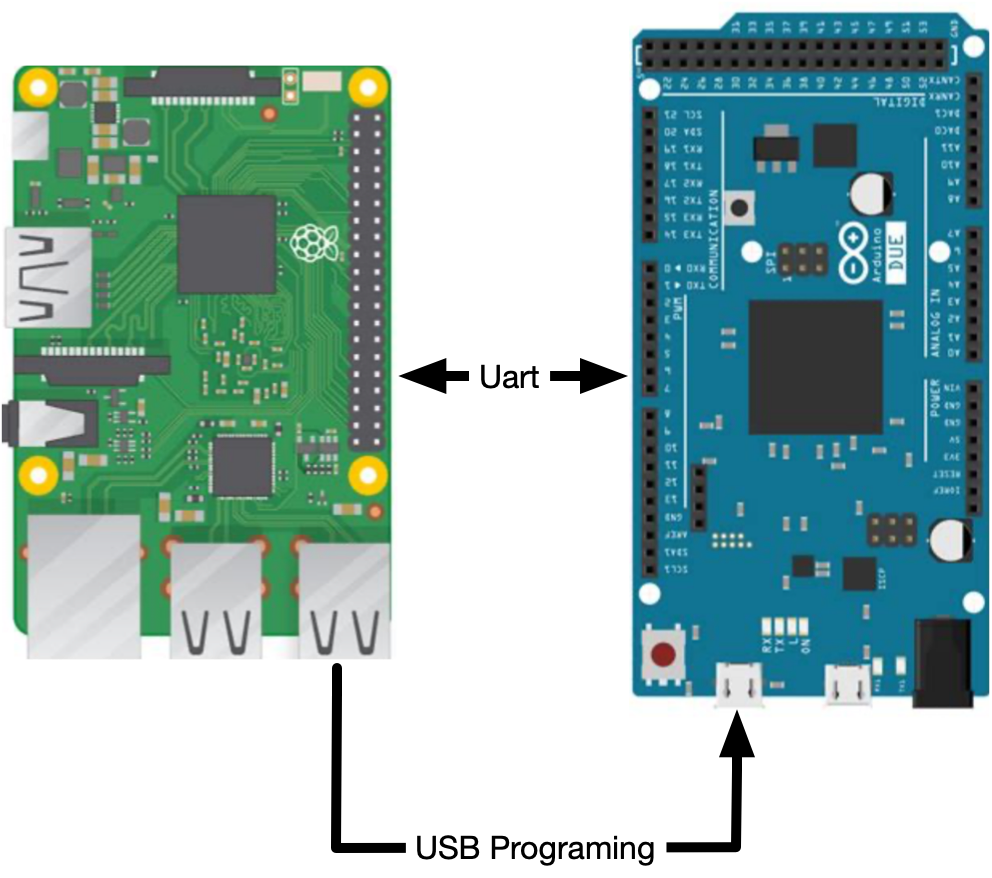
\includegraphics[width=0.85\linewidth]{Chapter-13/figs/test-platform.png}
  \caption{Hardware testbed: Raspberry Pi host (left) and Arduino Due target (right).
  The Raspberry Pi performs binary mutation, flashing, and data collection.
  The Arduino Due executes the boot sequence and returns status and SHA logs over UART.}
  \label{fig:testbed}
\end{figure}

The experimental setup consists of a \textbf{Raspberry Pi 4B} host and an
\textbf{Arduino Due (ATSAM3X8E)} target connected via USB and UART.  
The host manages all experimental control—performing binary mutation,
re-flashing the target, and capturing UART output—while the target executes
the instrumented firmware during each trial.

\paragraph{Host (Raspberry Pi 4B).}
Runs Python-based orchestration scripts on Raspberry Pi OS (64-bit, Debian Bookworm).  
The host coordinates all test automation, including mutation, flashing, log
capture, and SHA verification.

\paragraph{Target (Arduino Due).}
Features an ARM Cortex-M3 @ 84 MHz, with 512 KB of flash (read-only at runtime)
and 96 KB of SRAM (read-write).  
The target executes a two-stage boot sequence (B0 → B1 → RTOS) and reports
the computed SHA digest and status logs over UART.

\paragraph{Connections.}
\begin{itemize}
  \item \emph{USB (programming port)} — reprograms the target using BOSSA.
  \item \emph{UART (USART2 TXD: PD28 / RXD: PD30)} — dedicated link for telemetry and SHA output.
\end{itemize}

This hardware platform enables fully automated, repeatable testing runs,
which are described in detail in the following section.

% ---------------------------------------------------
\section{Evaluation Procedure}
\label{sec:evaluation-proc}

\begin{figure}[t]
  \centering
  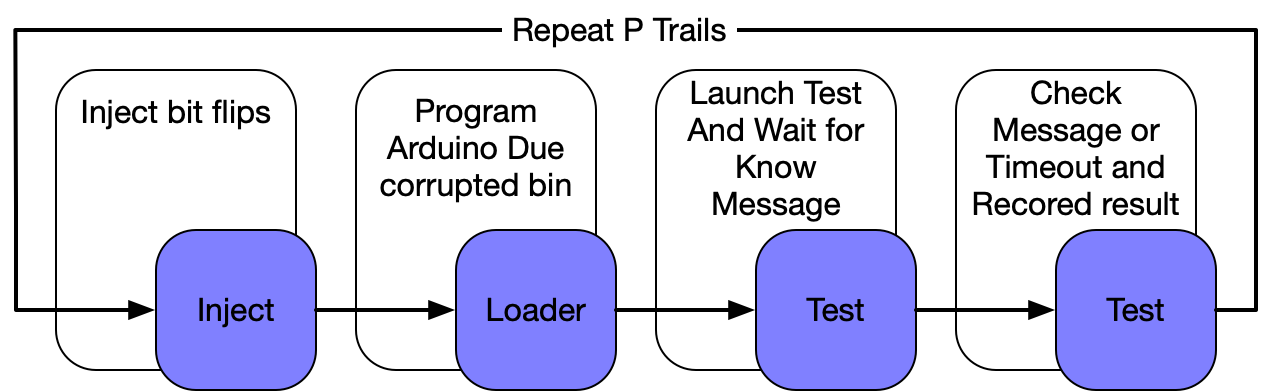
\includegraphics[width=0.9\linewidth]{Chapter-13/figs/test-sequence.png}
  \caption{Automated test sequence. Each iteration injects bit flips into the binary,
  flashes the target, executes the boot sequence, monitors UART output, and records success or failure.}
  \label{fig:test-sequence}
\end{figure}

The evaluation process measures system reliability under randomly injected bit
flips. Each trial executes a complete flash–boot–verify cycle controlled by
the host system. The entire process is automated and repeatable.

\begin{enumerate}
  \item Build the firmware image.
  \item Apply controlled bit flips to the image (fault injection step).
  \item Flash the mutated image to the target via USB.
  \item Boot the target and monitor UART output for SHA or status messages.
  \item Compare the reported SHA digest against the known reference to classify
        the result as \emph{success} or \emph{failure}.
\end{enumerate}

This procedure is repeated for multiple fault densities and random seeds to
capture statistical trends in reliability.

\subsection{Fault Injection}
\label{sec:fault-injection}

Faults are modeled as random bit flips applied directly to the firmware binary \emph{before flashing it to the target}.
Each experiment injects faults at a controlled density determined by the
parameter \(R\) (Bytes with a bit failure). Let \(B\) denote the size (in bytes) of the
tested region of the file.

\paragraph{Expected flips.}
\[
  E \;=\; \left\lceil \frac{B}{R} \right\rceil .
\]

\paragraph{Injection range.}
Bit positions are drawn from the contiguous range
\[
  k \in [\,0,\, E \cdot R \cdot 8\,),
\]
which corresponds to the mutation window of \(E \cdot R\) bytes.
This window is positioned to cover the code under test; only bit indices that
map into the file (\(k < B \cdot 8\)) are eligible. Any index with
\(k \ge B \cdot 8\) is ignored.

\paragraph{Random selection.}
For each trial, draw \(E\) independent integers
\[
  k_1, \dots, k_E \sim \mathrm{Uniform}\{0, \dots, E \cdot R \cdot 8 - 1\},
\]
and toggle the corresponding bits that fall within the file. Duplicate indices
naturally cancel under modulo-2 arithmetic.

\paragraph{Corruption model.}
Let \(X \in \{0,1\}^{B \cdot 8}\) be the original file bitstream; define
\[
  \widetilde{X}
  \;=\;
  X \;\oplus\; \bigoplus_{i=1}^{E} e_{k_i}
  \quad \text{with each term included only if } k_i < B \cdot 8.
\]
The mutated file \(\widetilde{X}\) is then flashed to the target, modeling
persistent (non-volatile) corruption in flash.



% ---------------------------------------------------
\section{System Boot Architecture}
\label{sec:system-boot-architecture}

The embedded system under test follows a two-stage boot architecture that
separates hardware initialization, memory relocation, and runtime execution.
This structure reflects the practical constraints of the ATSAM3X8E
microcontroller, where on-chip flash memory is \emph{read-only at runtime},
requiring executable code to be relocated into SRAM for modification or repair.

\begin{figure}[t]
  \centering
  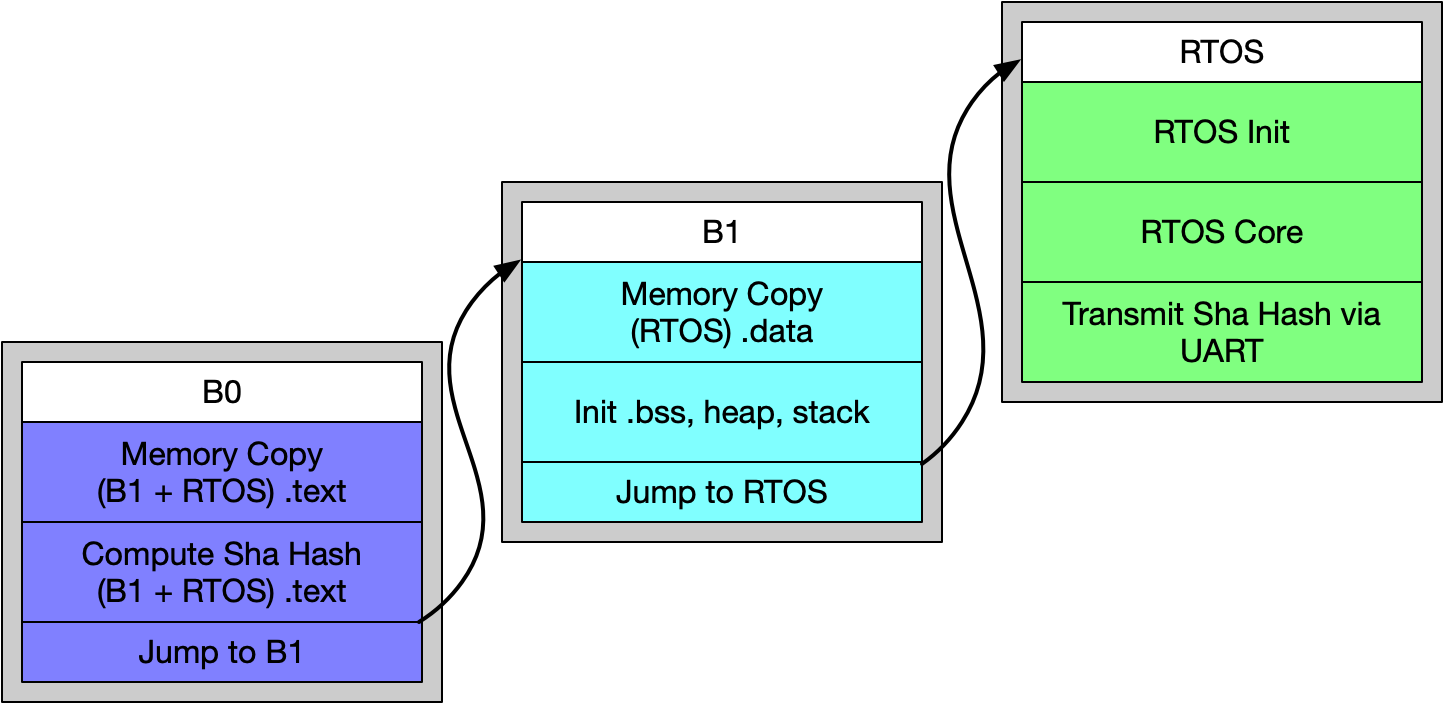
\includegraphics[width=0.95\linewidth]{Chapter-13/figs/boot-overview.png}
  \caption{Two-stage boot sequence showing flash-resident B0 and SRAM-resident
  B1 and RTOS stages. B0 relocates code and computes a SHA digest before
  transferring control to B1, which completes initialization and starts the RTOS.}
  \label{fig:system-boot-architecture}
\end{figure}

\begin{description}
  \item[Stage B0 (Bootloader).]
        Executes directly from flash at reset. B0 performs memory relocation by
        copying all executable sections of B1 and the RTOS (\texttt{.text} and
        \texttt{.rodata}) from flash into SRAM. Once relocation is complete, B0
        computes a SHA digest over the relocated regions and transfers control
        to B1.

  \item[Stage B1 (Application Loader).]
        Executes from SRAM. B1 completes runtime setup by copying
        \texttt{.data} to RAM, initializing \texttt{.bss}, allocating heap and
        stack space, and initializing the relocated vector table. When
        initialization is complete, control transfers to the RTOS initialization
        and kernel runtime.

  \item[RTOS / Runtime.]
        Runs entirely from SRAM. Initializes I/O interfaces and RTOS runtime
        configurations. After startup, the RTOS task begins transmitting the SHA
        digest computed by B0 over UART to the host, enabling the Raspberry Pi
        controller to verify code integrity and record system status.
\end{description}

This two-stage design isolates immutable boot logic (B0) from modifiable
runtime code (B1 and RTOS). Because the CPU cannot modify or write to flash at
runtime, all repair or redundancy mechanisms must operate on the SRAM-resident
images. B0 therefore remains fixed and responsible only for relocation and
validation, while B1 and the RTOS contain the hardened and repairable code
regions evaluated in subsequent sections. The SRAM serves as the writable proxy
for flash. In practice, flash would also be part of the repair domain; however,
its limited program/erase endurance would accelerate cell degradation across
many trials. Thus, performing updates in SRAM accurately models repair behavior
without introducing wear-out artifacts in the hardware.

\section{Basic System Configurations}
\label{sec:basic-configurations}

Two system configurations are evaluated to understand how memory access
restrictions affect the design and effectiveness of fault-tolerant mechanisms.
Both configurations employ an \textbf{Integrity Loader}—a minimal pre-boot
routine that executes before Stage~B0—to increase startup reliability and
establish a verified execution context prior to relocation.

Depending on hardware constraints, the Integrity Loader activates one of two
strategies:
\emph{repair-based hardening}, when writable memory regions are available, or
\emph{replication-based hardening}, when only read-only flash is accessible.
These complementary setups allow evaluation of fault-tolerance under both ideal
and realistic hardware conditions.

% ---------------------------------------------------
\subsection{Scenario A — Writable Flash (Emulated via SRAM)}
\label{sec:scenario-a}

In this configuration, the system emulates a device with writable flash memory,
allowing in-place code repair and recovery during runtime. Although the
ATSAM3X8E microcontroller supports self-programming through the EEFC interface,
repeated program/erase operations during fault-injection campaigns would
\emph{artificially degrade the flash memory}. To preserve device integrity and
enable large-scale experimentation, SRAM is used to \emph{emulate the
effectiveness of updateable flash memory}. All write and repair operations are
redirected to SRAM shadow regions that mirror the flash address layout,
providing an accurate model of in-place repair without incurring physical wear.

\begin{itemize}
  \item \textbf{Integrity Loader.}
        Executes from SRAM before B0. It validates the flash interface and
        initializes the writable SRAM shadow region that serves as a proxy for
        flash. This enables B0 and later stages to perform recovery actions
        as though flash were writable at runtime.

  \item \textbf{B0, B1, and RTOS.}
        All stages execute with writable counterparts mapped into SRAM. During
        recovery, corrupted regions may be repaired by rewriting code or
        metadata within the shadow copy while maintaining the same logical
        structure as flash. Replication can operate alongside repair, forming
        hybrid recovery strategies.

  \item \textbf{Runtime properties.}
        \begin{itemize}
          \item Flash updates are emulated through SRAM shadow regions.
          \item Prevents artificial flash wear during large-scale experiments.
          \item Enables combined evaluation of repair and replication methods.
        \end{itemize}
\end{itemize}

This configuration emulates the operational benefits of having writable flash,
allowing repair-based fault recovery to be tested under conditions equivalent
to a system with full nonvolatile write capability, but without physically
reprogramming flash.


% ---------------------------------------------------
\subsection{Scenario B — Flash Read-Only (Locked System)}
\label{sec:scenario-b}

In this configuration, flash memory is hardware-locked and cannot be modified
while executing. Only SRAM regions are writable, requiring fault recovery to
rely exclusively on replication and redirection rather than in-place repair.

\begin{itemize}
  \item \textbf{Integrity Loader.}
        Executes before B0 to verify that flash contents are consistent and
        readable. Since flash cannot be rewritten, the loader transitions to a
        \emph{replication-based initialization role}, preparing SRAM to receive
        relocated and validated copies of B1 and RTOS code prior to execution.

  \item \textbf{B0, B1, and RTOS.}
        B0 remains fixed in flash and performs relocation only. B1 and RTOS are
        loaded into SRAM, where replication-based hardening (e.g., FLCR or
        majority-voting mechanisms) provides resilience. Fault recovery occurs
        through runtime redirection to verified replicas instead of modification.

  \item \textbf{Runtime properties.}
        \begin{itemize}
          \item Flash is read-only during execution.
          \item Recovery achieved solely through replication and redirection.
          \item Integrity Loader validates flash and initializes replication tables.
        \end{itemize}
\end{itemize}

This configuration reflects the behavior of real embedded systems with
read-only flash, such as the ATSAM3X8E. Here, resilience is achieved entirely
through replication-based mechanisms in SRAM-resident code, isolating runtime
recovery from immutable flash contents.

% ---------------------------------------------------
\subsection*{Configuration Summary}

\begin{table}[h!]
  \centering
  \renewcommand{\arraystretch}{1.15}
  \begin{tabularx}{\linewidth}{|l|c|c|X|}
    \hline
    \textbf{Region} & \textbf{Exec Location} & \textbf{Writable at Runtime} & \textbf{Applicable Techniques} \\ \hline
    \multicolumn{4}{|l|}{\textbf{Scenario A — Flash Fully Writable (Unlocked System)}} \\ \hline
    B0        & Flash/SRAM & Yes & Repair; Replication (FLCR/BBLCR) \\ \hline
    B1, RTOS  & SRAM       & Yes & Repair; Replication (FLCR/BBLCR) \\ \hline
    \multicolumn{4}{|l|}{\textbf{Scenario B — Flash Read-Only (Locked Bootloader)}} \\ \hline
    B0        & Flash & No  & Immutable; validated via SHA \\ \hline
    B1, RTOS  & SRAM  & Yes & Repair; Replication (FLCR/BBLCR) \\ \hline
  \end{tabularx}
  \caption{Runtime writability and hardening capabilities for the two system configurations.}
  \label{tab:system-access-configs}
\end{table}


% ---------------------------------------------------
\section{Protection Domains and Strategy}
\label{sec:protection-domains}

The CPU executes directly from flash at reset, but flash is not writable at runtime; SRAM is writable. This yields two protection domains:
\begin{itemize}
  \item \textbf{Flash (non-writable):} B0 resides/executes here. Fault tolerance uses \emph{replication + redirection} (e.g., FLCR) rather than in-place repair.
  \item \textbf{SRAM (writable):} B1 and RTOS are relocated here. Fault tolerance can use \emph{replication + repair} (e.g., majority voting) on runtime-modifiable code.
\end{itemize}
The configurations below combine these mechanisms across domains.

% ---------------------------------------------------
\section{Test Configurations}
\label{sec:test-configs}

\begin{description}
  \item[Baseline:] No replication or runtime repair; serves as the reference.
  \item[Majority of 3 (B1 + RTOS):] Triplication and majority voting applied to B1 and RTOS (relocated to SRAM); B0 remains baseline.
  \item[Dual Image:] Two complete images in flash; if B0’s SHA check fails on the primary, B0 boots the alternate.
  \item[\( \text{FLCR(B0)} + \text{Majority(B1+RTOS)} \):] B0 uses Function-Level Code Replication (redirection across replicas in flash). B1 and RTOS use Majority-of-3 in SRAM.
\end{description}

% ---------------------------------------------------
\section{Hardened System Overview}
\label{sec:hardened-overview}

Hardening introduces:
\begin{itemize}
  \item \textbf{Boot redirection (B0/flash):} Call sites in B0 resolve through an indirection table populated at startup, allowing control to skip corrupted function copies.
  \item \textbf{Runtime repair (B1+RTOS/SRAM):} Triplicated functions execute under majority voting to mask transient or localized corruption after relocation.
  \item \textbf{Startup ordering:} B0 initializes its redirection metadata before handing off; B1 initializes replicated state and voting logic after relocation.
\end{itemize}

% ---------------------------------------------------
\section{Memory Overview}
\label{sec:memory-overview}

\subsection{Baseline}
\label{sec:memory-baseline}

\begin{figure}[t]
  \centering
  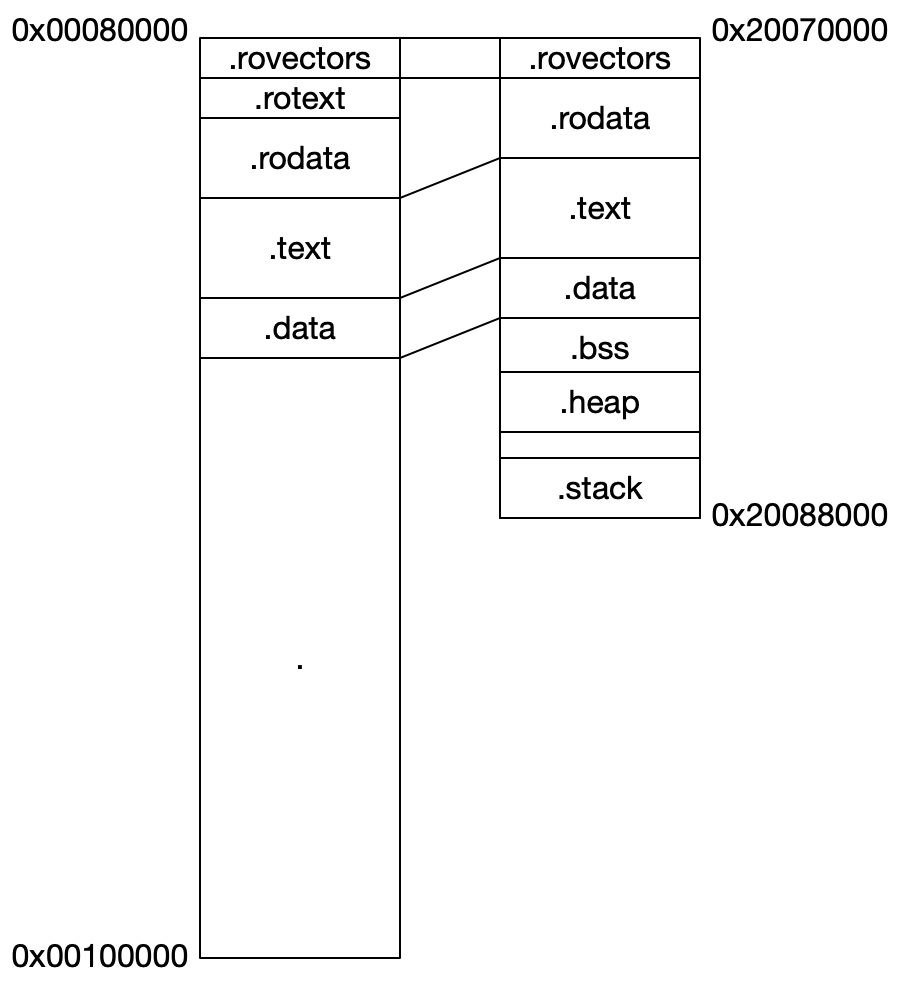
\includegraphics[width=0.72\linewidth]{Chapter-13/figs/baseline-memory.png}
  \caption{Baseline memory layout. At reset B0 copies \texttt{.rovector}, \texttt{.text}, \texttt{.rodata}, \texttt{.data} from flash to SRAM; \texttt{.bss}/heap/stack are created in SRAM; execution proceeds from SRAM.}
  \label{fig:baseline-memory}
\end{figure}

\noindent \textbf{Flash:} persistent copies of \texttt{.rovector}, \texttt{.text}, \texttt{.rodata}, \texttt{.data}. \;
\textbf{SRAM:} relocated code/data plus \texttt{.bss}/heap/stack. \;
No runtime indirection beyond B0’s SHA check.

\subsection{Majority of 3 (B1 + RTOS)}
\label{sec:memory-maj}
B1 and RTOS \texttt{.text} are relocated to SRAM as three replicas per protected function; voter state and minimal metadata reside in SRAM. Flash holds the single persistent image; only one working set is executed from SRAM.

\subsection{Dual Image}
\label{sec:memory-dual}
Flash stores two full images (primary/alternate). B0 executes from flash, validates the selected image, and relocates that image’s \texttt{.text}/\texttt{.data} to SRAM. Only one image is active in SRAM at a time.

\subsection{\( \text{FLCR(B0)} + \text{Majority(B1+RTOS)} \)}
\label{sec:memory-hybrid}
B0 executes from flash with function replicas present in flash and an indirection table/metadata initialized at startup. B1+RTOS relocate to SRAM with triplicated functions and voter logic resident in SRAM. This combines flash-domain redirection with SRAM-domain repair.

% ---------------------------------------------------
\section{Results (placeholder)}
\label{sec:results}
% (Insert reliability curves, overhead tables, and failure-mode histograms.)

\textbf{Planned outputs:} \(\rho(R)\) vs.\ \(R\) for all configurations; boot time and RAM/flash overheads; failure classifications (boot fail / wrong SHA / hang).

% ---------------------------------------------------
\section{Summary}
\label{sec:case-summary}
We defined a consistent hardware automation loop, embedded baseline, and hybrid protection strategy driven by memory writability. Four configurations—Baseline, Majority(B1+RTOS), Dual Image, and \(\text{FLCR(B0)}+\text{Majority(B1+RTOS)}\)—are tested under identical, randomized fault populations using a repeat-\(P\) procedure. Results (next draft) will compare reliability and overhead trade-offs across these approaches.
%%---------------------------------------------------------------------------%%
%%  Bibliography 
%% or use BibTeX
\bibliography{StudentName-thesis}
\bibliographystyle{apalike}

%%---------------------------------------------------------------------------%%
% Appendices
%\ensureoddstart
\restoregeometry
\appendix
%\newgeometry{margin=1in,lmargin=1.25in,footskip=\chapterfootskip, includehead, includefoot}

% Can remove or add
\include{Appendix-A/Appendix-A}
\include{Appendix-B/Appendix-B}

\restoregeometry

%%---------------------------------------------------------------------------%%

%%---------------------------------------------------------------------------%%
\backmatter

\end{document}